% !TEX program = xelatex
% ---------------------------------------------------------------------------
%  DSA in Python -- revision flashcards (Beamer)
%  Compile with XeLaTeX (or LuaLaTeX):   xelatex dsa_flashcards.tex
%  Every card = 2 slides: a dark QUESTION slide, then a light ANSWER slide.
%  Fonts: uses Inter + DejaVu Sans Mono if installed; otherwise falls back
%  to Latin Modern, which ships with every TeX distribution.
% ---------------------------------------------------------------------------
\documentclass[aspectratio=1610,11pt]{beamer}

\usepackage{fontspec}
\usepackage[table]{xcolor}
\usepackage{tikz}
\usetikzlibrary{calc}
\usepackage{tcolorbox}
\tcbuselibrary{skins}
\usepackage{listings}
\usepackage{booktabs}
\usepackage{array}

% ---- fonts (with graceful fallbacks) --------------------------------------
\IfFontExistsTF{Inter}{%
  \setsansfont{Inter}[Ligatures=TeX]%
}{%
  \setsansfont{Latin Modern Sans}[Ligatures=TeX]%
}
\IfFontExistsTF{DejaVu Sans Mono}{%
  \setmonofont{DejaVu Sans Mono}[Scale=MatchLowercase]%
}{\IfFontExistsTF{Menlo}{%
  \setmonofont{Menlo}[Scale=MatchLowercase]%
}{\IfFontExistsTF{Consolas}{%
  \setmonofont{Consolas}[Scale=MatchLowercase]%
}{%
  \setmonofont{Latin Modern Mono}%
}}}
\renewcommand{\familydefault}{\sfdefault}

% ---- palette ----------------------------------------------------------------
\definecolor{ink}{HTML}{0B1220}        % question-slide background
\definecolor{snow}{HTML}{F8FAFC}       % text on dark
\definecolor{paper}{HTML}{F7F5F0}      % answer-slide background
\definecolor{inkt}{HTML}{1E293B}       % text on light
\definecolor{mutedf}{HTML}{94A3B8}     % muted on dark
\definecolor{mutedb}{HTML}{64748B}     % muted on light
\definecolor{codebg}{HTML}{111A2E}
\definecolor{codefg}{HTML}{E2E8F0}
\definecolor{kw}{HTML}{F472B6}
\definecolor{bi}{HTML}{7DD3FC}
\definecolor{slf}{HTML}{A5B4FC}
\definecolor{strc}{HTML}{FCD34D}
\definecolor{cmt}{HTML}{8394B0}
\definecolor{warnbg}{HTML}{FEF3C7}
\definecolor{warnbar}{HTML}{B45309}
\definecolor{rowtint}{HTML}{EFEBE3}
\definecolor{rulec}{HTML}{CFC8BA}
\definecolor{s0}{HTML}{F5B83D}\definecolor{s1}{HTML}{2DD4BF}\definecolor{s2}{HTML}{FB7185}
\definecolor{s3}{HTML}{A78BFA}\definecolor{s4}{HTML}{38BDF8}\definecolor{s5}{HTML}{A3E635}
% placeholders, overridden for every card
\definecolor{acc}{HTML}{F5B83D}
\definecolor{accd}{HTML}{B45309}
\newcommand{\mutedc}{mutedb}
\newcommand{\figc}{accd}
\newcommand{\codecolor}{accd}

% ---- beamer set-up ----------------------------------------------------------
\setbeamertemplate{navigation symbols}{}
\setbeamertemplate{headline}{}
\setbeamertemplate{footline}{}
\setbeamersize{text margin left=13mm,text margin right=13mm}
\setbeamertemplate{itemize item}{\raisebox{0.2ex}{\color{accd}\fontsize{5}{5}\selectfont$\blacksquare$}}
\setbeamertemplate{itemize subitem}{\raisebox{0.2ex}{\color{accd}\fontsize{4}{4}\selectfont$\blacksquare$}}
\makeatletter\newcommand{\tilelink}[2]{\hyper@linkstart{link}{#1}#2\hyper@linkend}\makeatother
\hypersetup{pdftitle={DSA in Python -- Flashcards},hidelinks}

% ---- small helpers ----------------------------------------------------------
\frenchspacing
\hyphenpenalty=10000\exhyphenpenalty=10000
\newcommand{\code}[1]{\textcolor{\codecolor}{\texttt{#1}}}

% top row, progress bar, index link.  #1 pill text, #2 counter, #3 progress 0-1
\newcommand{\chrome}[3]{%
\begin{tikzpicture}[remember picture,overlay]
  \node[anchor=north west,fill=acc,text=ink,rounded corners=1.5mm,inner xsep=2.4mm,
        inner ysep=1.3mm,font=\fontsize{7}{8}\selectfont\bfseries]
       at ($(current page.north west)+(13mm,-6mm)$) {\MakeUppercase{#1}};
  \node[anchor=north east,text=\mutedc,font=\fontsize{7}{8}\selectfont\ttfamily]
       at ($(current page.north east)+(-13mm,-6.6mm)$) {#2};
  \fill[\mutedc!28] (current page.south west) rectangle ($(current page.south west)+(\paperwidth,1.2mm)$);
  \fill[acc] (current page.south west) rectangle ($(current page.south west)+(#3\paperwidth,1.2mm)$);
  \node[anchor=south east,font=\fontsize{6.5}{8}\selectfont,text=\mutedc]
       at ($(current page.south east)+(-13mm,3mm)$) {\hyperlink{index}{index}};
\end{tikzpicture}}

% small "EXTRA" tag for cards that are not in the original notes
\newcommand{\extratag}{%
\begin{tikzpicture}[remember picture,overlay]
  \node[anchor=north east,draw=acc,text=acc,rounded corners=1.5mm,inner xsep=2mm,inner ysep=1mm,
        font=\fontsize{6.5}{8}\selectfont\bfseries]
       at ($(current page.north east)+(-33mm,-6.1mm)$) {EXTRA \textperiodcentered\ NOT IN YOUR NOTES};
\end{tikzpicture}}

\newcommand{\fliphint}{%
\begin{tikzpicture}[remember picture,overlay]
  \node[anchor=south,text=\mutedc,font=\fontsize{7}{8}\selectfont]
       at ($(current page.south)+(0,3mm)$) {think it through, then flip $\rightarrow$};
\end{tikzpicture}}

% code panel
\lstdefinestyle{dsa}{language=Python,
  basicstyle=\ttfamily\color{codefg},
  keywordstyle=\color{kw},
  keywordstyle=[2]\color{bi},
  keywordstyle=[3]\color{slf},
  commentstyle=\color{cmt}\itshape,
  stringstyle=\color{strc},
  morekeywords={True,False,None,nonlocal},
  morekeywords=[2]{len,range,print,min,max,sorted,list,set,dict,enumerate,float,int,str,abs,
    isinstance,chr,ord,sum,tuple,bool,deque,defaultdict,Counter,IndexError,OverflowError,
    ValueError,TypeError,KeyError,heappush,heappop,List},
  morekeywords=[3]{self},
  showstringspaces=false,columns=fixed,keepspaces=true,
  aboveskip=0pt,belowskip=0pt,xleftmargin=0pt,xrightmargin=0pt}
\lstset{style=dsa}
\newtcolorbox{codebox}{enhanced,colback=codebg,colframe=codebg,boxrule=0pt,arc=2.4mm,
  left=3mm,right=3mm,top=2.2mm,bottom=2.2mm,boxsep=0pt,before skip=0pt,after skip=0pt}
\newtcolorbox{notebox}{enhanced,colback=warnbg,colframe=warnbg,boxrule=0pt,arc=1.8mm,
  borderline west={1.6mm}{0pt}{warnbar},left=4mm,right=3mm,top=1.6mm,bottom=1.6mm,boxsep=0pt,
  before skip=0pt,after skip=0pt}

% ---- figures used on some cards ------------------------------------------------
\newcommand{\treefig}{%
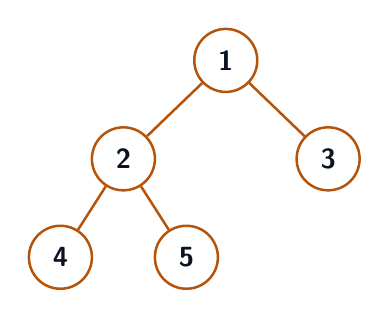
\begin{tikzpicture}[tn/.style={circle,draw=\figc,fill=white,line width=0.9pt,minimum size=8mm,
    inner sep=0pt,font=\bfseries\color{ink}}]
  \node[tn] (t1) at (0,0) {1};
  \node[tn] (t2) at (-1.3,-1.25) {2};
  \node[tn] (t3) at (1.3,-1.25) {3};
  \node[tn] (t4) at (-2.1,-2.5) {4};
  \node[tn] (t5) at (-0.5,-2.5) {5};
  \foreach \a/\b in {1/2,1/3,2/4,2/5}{\draw[line width=0.9pt,draw=\figc] (t\a)--(t\b);}
\end{tikzpicture}}

\newcommand{\graphfig}{%
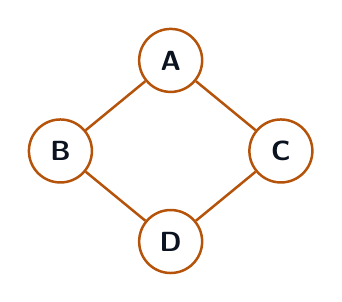
\begin{tikzpicture}[gn/.style={circle,draw=\figc,fill=white,line width=0.9pt,minimum size=8mm,
    inner sep=0pt,font=\bfseries\color{ink}}]
  \node[gn] (A) at (0,1.15) {A};
  \node[gn] (B) at (-1.4,0) {B};
  \node[gn] (C) at (1.4,0) {C};
  \node[gn] (D) at (0,-1.15) {D};
  \draw[line width=0.9pt,draw=\figc] (A)--(B) (A)--(C) (B)--(D) (C)--(D);
\end{tikzpicture}}

\newcommand{\heapfig}{%
\scalebox{0.82}{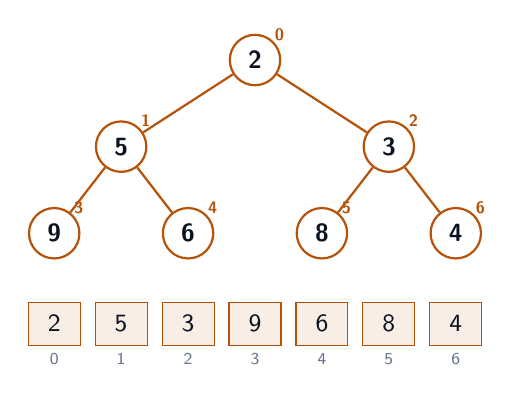
\begin{tikzpicture}[hn/.style={circle,draw=\figc,fill=white,line width=0.8pt,minimum size=6.4mm,
    inner sep=0pt,font=\small\bfseries\color{ink}},ix/.style={font=\fontsize{6}{7}\selectfont\bfseries,text=accd}]
  \node[hn] (n0) at (0,0) {2};
  \node[hn] (n1) at (-1.7,-1.1) {5};
  \node[hn] (n2) at (1.7,-1.1) {3};
  \node[hn] (n3) at (-2.55,-2.2) {9};
  \node[hn] (n4) at (-0.85,-2.2) {6};
  \node[hn] (n5) at (0.85,-2.2) {8};
  \node[hn] (n6) at (2.55,-2.2) {4};
  \foreach \a/\b in {0/1,0/2,1/3,1/4,2/5,2/6}{\draw[line width=0.8pt,draw=\figc] (n\a)--(n\b);}
  \foreach \i in {0,...,6}{\node[ix,anchor=south west,inner sep=0.3pt] at (n\i.north east) {\i};}
  \foreach \v [count=\i from 0] in {2,5,3,9,6,8,4}{%
    \node[draw=accd,fill=accd!10,minimum width=6.6mm,minimum height=5.4mm,inner sep=0pt,
      font=\small\color{ink}] (a\i) at ({-2.55+0.85*\i},-3.35) {\v};
    \node[font=\fontsize{6}{7}\selectfont,text=mutedb,anchor=north] at ($(a\i.south)+(0,0.2mm)$) {\i};}
\end{tikzpicture}}}

\begin{document}


%% ================= title =================
{\setbeamercolor{background canvas}{bg=ink}\setbeamercolor{normal text}{fg=snow}
\definecolor{acc}{HTML}{F5B83D}\definecolor{accd}{HTML}{B45309}
\renewcommand{\mutedc}{mutedf}\renewcommand{\figc}{acc}\renewcommand{\codecolor}{acc}
\begin{frame}[plain,c]
\begin{tikzpicture}[remember picture,overlay]
  \foreach \k in {0,...,5}{
    \fill[s\k] ($(current page.south west)+({13mm+\k*14mm},0)$) rectangle ++(14mm,2.4mm);
  }
\end{tikzpicture}
\noindent{\fontsize{8.5}{10}\selectfont\bfseries\color{acc}REVISION FLASHCARDS}\par\vspace{3mm}
{\fontsize{40}{44}\selectfont\bfseries\color{snow}DSA in Python}\par\vspace{4mm}
{\fontsize{15}{20}\selectfont\color{mutedf}Dicts and sets to graphs and bit tricks}\par\vspace{3mm}
{\fontsize{10}{14}\selectfont\ttfamily\color{acc}133 cards \textperiodcentered\ 12 topics \textperiodcentered\ question $\rightarrow$ answer}\par
\end{frame}
}

%% ================= how to use =================
{\setbeamercolor{background canvas}{bg=ink}\setbeamercolor{normal text}{fg=snow}
\definecolor{acc}{HTML}{2DD4BF}\definecolor{accd}{HTML}{0F766E}
\renewcommand{\mutedc}{mutedf}\renewcommand{\figc}{acc}\renewcommand{\codecolor}{acc}
\begin{frame}[plain,c]
\begin{tikzpicture}[remember picture,overlay]
  \fill[acc] (current page.south west) rectangle ($(current page.south west)+(\paperwidth,1.2mm)$);
\end{tikzpicture}
\noindent{\fontsize{8.5}{10}\selectfont\bfseries\color{acc}HOW TO USE THIS DECK}\par\vspace{4mm}
{\fontsize{24}{29}\selectfont\bfseries\color{snow}Every card is two slides.}\par\vspace{6mm}
\begin{minipage}[t]{0.31\textwidth}\raggedright
{\fontsize{26}{28}\selectfont\bfseries\color{acc}1}\par\vspace{1mm}
\textbf{Question} \textemdash\ a dark slide. Answer out loud, or write the code on paper, \emph{before} you flip.
\end{minipage}\hfill
\begin{minipage}[t]{0.31\textwidth}\raggedright
{\fontsize{26}{28}\selectfont\bfseries\color{acc}2}\par\vspace{1mm}
\textbf{Answer} \textemdash\ the light slide that follows. Compare line by line, and note what you missed.
\end{minipage}\hfill
\begin{minipage}[t]{0.31\textwidth}\raggedright
{\fontsize{26}{28}\selectfont\bfseries\color{acc}3}\par\vspace{1mm}
\textbf{Navigate} \textemdash\ every slide has an \texttt{index} link at the bottom right that jumps to the topic list.
\end{minipage}\par\vspace{7mm}
{\fontsize{10}{14}\selectfont\color{mutedf}Cards tagged \textbf{EXTRA} were added on top of your notes. Amber boxes (\textbf{WATCH OUT}) flag common slips.}
\end{frame}
}


%% ================= index =================
{\setbeamercolor{background canvas}{bg=ink}\setbeamercolor{normal text}{fg=snow}
\definecolor{acc}{HTML}{F5B83D}\definecolor{accd}{HTML}{B45309}
\renewcommand{\mutedc}{mutedf}\renewcommand{\figc}{acc}\renewcommand{\codecolor}{acc}
\begin{frame}[plain,c]
\hypertarget{index}{}
\begin{tikzpicture}[remember picture,overlay]
  \node[anchor=north west,text=acc,font=\fontsize{8.5}{10}\selectfont\bfseries] at ($(current page.north west)+(13mm,-7mm)$) {TOPICS \textperiodcentered\ CLICK TO JUMP};
  \node[anchor=north west,text=snow,font=\fontsize{20}{24}\selectfont\bfseries] at ($(current page.north west)+(13mm,-12.5mm)$) {Index};
\definecolor{t0}{HTML}{F5B83D}
\node[anchor=north west,fill=white!7!ink,rounded corners=2mm,minimum width=33.5mm,minimum height=21.5mm,inner sep=0pt] (tile0) at ($(current page.north west)+(13.0mm,-22.5mm)$) {};
\fill[t0,rounded corners=0.6mm] (tile0.north west) rectangle ++(33.5mm,-1.1mm);
\node[anchor=north west,inner xsep=2.6mm,inner ysep=2.6mm,align=left,text=snow] at (tile0.north west) {\tilelink{sec1}{\parbox{28.3mm}{\raggedright{\fontsize{7}{8}\selectfont\ttfamily\color{t0}01}\par\vspace{0.6mm}{\fontsize{9.5}{11}\selectfont\bfseries\color{snow}Dicts \& Sets}\par\vspace{0.8mm}{\fontsize{7}{8}\selectfont\color{mutedf}8 cards}}}};

\definecolor{t1}{HTML}{2DD4BF}
\node[anchor=north west,fill=white!7!ink,rounded corners=2mm,minimum width=33.5mm,minimum height=21.5mm,inner sep=0pt] (tile1) at ($(current page.north west)+(50.1mm,-22.5mm)$) {};
\fill[t1,rounded corners=0.6mm] (tile1.north west) rectangle ++(33.5mm,-1.1mm);
\node[anchor=north west,inner xsep=2.6mm,inner ysep=2.6mm,align=left,text=snow] at (tile1.north west) {\tilelink{sec2}{\parbox{28.3mm}{\raggedright{\fontsize{7}{8}\selectfont\ttfamily\color{t1}02}\par\vspace{0.6mm}{\fontsize{9.5}{11}\selectfont\bfseries\color{snow}Arrays}\par\vspace{0.8mm}{\fontsize{7}{8}\selectfont\color{mutedf}10 cards}}}};

\definecolor{t2}{HTML}{FB7185}
\node[anchor=north west,fill=white!7!ink,rounded corners=2mm,minimum width=33.5mm,minimum height=21.5mm,inner sep=0pt] (tile2) at ($(current page.north west)+(87.2mm,-22.5mm)$) {};
\fill[t2,rounded corners=0.6mm] (tile2.north west) rectangle ++(33.5mm,-1.1mm);
\node[anchor=north west,inner xsep=2.6mm,inner ysep=2.6mm,align=left,text=snow] at (tile2.north west) {\tilelink{sec3}{\parbox{28.3mm}{\raggedright{\fontsize{7}{8}\selectfont\ttfamily\color{t2}03}\par\vspace{0.6mm}{\fontsize{9.5}{11}\selectfont\bfseries\color{snow}Strings}\par\vspace{0.8mm}{\fontsize{7}{8}\selectfont\color{mutedf}13 cards}}}};

\definecolor{t3}{HTML}{A78BFA}
\node[anchor=north west,fill=white!7!ink,rounded corners=2mm,minimum width=33.5mm,minimum height=21.5mm,inner sep=0pt] (tile3) at ($(current page.north west)+(124.3mm,-22.5mm)$) {};
\fill[t3,rounded corners=0.6mm] (tile3.north west) rectangle ++(33.5mm,-1.1mm);
\node[anchor=north west,inner xsep=2.6mm,inner ysep=2.6mm,align=left,text=snow] at (tile3.north west) {\tilelink{sec4}{\parbox{28.3mm}{\raggedright{\fontsize{7}{8}\selectfont\ttfamily\color{t3}04}\par\vspace{0.6mm}{\fontsize{9.5}{11}\selectfont\bfseries\color{snow}Sorting}\par\vspace{0.8mm}{\fontsize{7}{8}\selectfont\color{mutedf}16 cards}}}};

\definecolor{t4}{HTML}{38BDF8}
\node[anchor=north west,fill=white!7!ink,rounded corners=2mm,minimum width=33.5mm,minimum height=21.5mm,inner sep=0pt] (tile4) at ($(current page.north west)+(13.0mm,-47.0mm)$) {};
\fill[t4,rounded corners=0.6mm] (tile4.north west) rectangle ++(33.5mm,-1.1mm);
\node[anchor=north west,inner xsep=2.6mm,inner ysep=2.6mm,align=left,text=snow] at (tile4.north west) {\tilelink{sec5}{\parbox{28.3mm}{\raggedright{\fontsize{7}{8}\selectfont\ttfamily\color{t4}05}\par\vspace{0.6mm}{\fontsize{9.5}{11}\selectfont\bfseries\color{snow}Linked Lists}\par\vspace{0.8mm}{\fontsize{7}{8}\selectfont\color{mutedf}7 cards}}}};

\definecolor{t5}{HTML}{A3E635}
\node[anchor=north west,fill=white!7!ink,rounded corners=2mm,minimum width=33.5mm,minimum height=21.5mm,inner sep=0pt] (tile5) at ($(current page.north west)+(50.1mm,-47.0mm)$) {};
\fill[t5,rounded corners=0.6mm] (tile5.north west) rectangle ++(33.5mm,-1.1mm);
\node[anchor=north west,inner xsep=2.6mm,inner ysep=2.6mm,align=left,text=snow] at (tile5.north west) {\tilelink{sec6}{\parbox{28.3mm}{\raggedright{\fontsize{7}{8}\selectfont\ttfamily\color{t5}06}\par\vspace{0.6mm}{\fontsize{9.5}{11}\selectfont\bfseries\color{snow}Queues \& Deques}\par\vspace{0.8mm}{\fontsize{7}{8}\selectfont\color{mutedf}14 cards}}}};

\definecolor{t6}{HTML}{F5B83D}
\node[anchor=north west,fill=white!7!ink,rounded corners=2mm,minimum width=33.5mm,minimum height=21.5mm,inner sep=0pt] (tile6) at ($(current page.north west)+(87.2mm,-47.0mm)$) {};
\fill[t6,rounded corners=0.6mm] (tile6.north west) rectangle ++(33.5mm,-1.1mm);
\node[anchor=north west,inner xsep=2.6mm,inner ysep=2.6mm,align=left,text=snow] at (tile6.north west) {\tilelink{sec7}{\parbox{28.3mm}{\raggedright{\fontsize{7}{8}\selectfont\ttfamily\color{t6}07}\par\vspace{0.6mm}{\fontsize{9.5}{11}\selectfont\bfseries\color{snow}Stacks}\par\vspace{0.8mm}{\fontsize{7}{8}\selectfont\color{mutedf}5 cards}}}};

\definecolor{t7}{HTML}{2DD4BF}
\node[anchor=north west,fill=white!7!ink,rounded corners=2mm,minimum width=33.5mm,minimum height=21.5mm,inner sep=0pt] (tile7) at ($(current page.north west)+(124.3mm,-47.0mm)$) {};
\fill[t7,rounded corners=0.6mm] (tile7.north west) rectangle ++(33.5mm,-1.1mm);
\node[anchor=north west,inner xsep=2.6mm,inner ysep=2.6mm,align=left,text=snow] at (tile7.north west) {\tilelink{sec8}{\parbox{28.3mm}{\raggedright{\fontsize{7}{8}\selectfont\ttfamily\color{t7}08}\par\vspace{0.6mm}{\fontsize{9.5}{11}\selectfont\bfseries\color{snow}Heaps \& Priority Queues}\par\vspace{0.8mm}{\fontsize{7}{8}\selectfont\color{mutedf}10 cards}}}};

\definecolor{t8}{HTML}{FB7185}
\node[anchor=north west,fill=white!7!ink,rounded corners=2mm,minimum width=33.5mm,minimum height=21.5mm,inner sep=0pt] (tile8) at ($(current page.north west)+(13.0mm,-71.5mm)$) {};
\fill[t8,rounded corners=0.6mm] (tile8.north west) rectangle ++(33.5mm,-1.1mm);
\node[anchor=north west,inner xsep=2.6mm,inner ysep=2.6mm,align=left,text=snow] at (tile8.north west) {\tilelink{sec9}{\parbox{28.3mm}{\raggedright{\fontsize{7}{8}\selectfont\ttfamily\color{t8}09}\par\vspace{0.6mm}{\fontsize{9.5}{11}\selectfont\bfseries\color{snow}Binary Trees}\par\vspace{0.8mm}{\fontsize{7}{8}\selectfont\color{mutedf}14 cards}}}};

\definecolor{t9}{HTML}{A78BFA}
\node[anchor=north west,fill=white!7!ink,rounded corners=2mm,minimum width=33.5mm,minimum height=21.5mm,inner sep=0pt] (tile9) at ($(current page.north west)+(50.1mm,-71.5mm)$) {};
\fill[t9,rounded corners=0.6mm] (tile9.north west) rectangle ++(33.5mm,-1.1mm);
\node[anchor=north west,inner xsep=2.6mm,inner ysep=2.6mm,align=left,text=snow] at (tile9.north west) {\tilelink{sec10}{\parbox{28.3mm}{\raggedright{\fontsize{7}{8}\selectfont\ttfamily\color{t9}10}\par\vspace{0.6mm}{\fontsize{9.5}{11}\selectfont\bfseries\color{snow}Binary Search Trees}\par\vspace{0.8mm}{\fontsize{7}{8}\selectfont\color{mutedf}8 cards}}}};

\definecolor{t10}{HTML}{38BDF8}
\node[anchor=north west,fill=white!7!ink,rounded corners=2mm,minimum width=33.5mm,minimum height=21.5mm,inner sep=0pt] (tile10) at ($(current page.north west)+(87.2mm,-71.5mm)$) {};
\fill[t10,rounded corners=0.6mm] (tile10.north west) rectangle ++(33.5mm,-1.1mm);
\node[anchor=north west,inner xsep=2.6mm,inner ysep=2.6mm,align=left,text=snow] at (tile10.north west) {\tilelink{sec11}{\parbox{28.3mm}{\raggedright{\fontsize{7}{8}\selectfont\ttfamily\color{t10}11}\par\vspace{0.6mm}{\fontsize{9.5}{11}\selectfont\bfseries\color{snow}Graphs}\par\vspace{0.8mm}{\fontsize{7}{8}\selectfont\color{mutedf}18 cards}}}};

\definecolor{t11}{HTML}{A3E635}
\node[anchor=north west,fill=white!7!ink,rounded corners=2mm,minimum width=33.5mm,minimum height=21.5mm,inner sep=0pt] (tile11) at ($(current page.north west)+(124.3mm,-71.5mm)$) {};
\fill[t11,rounded corners=0.6mm] (tile11.north west) rectangle ++(33.5mm,-1.1mm);
\node[anchor=north west,inner xsep=2.6mm,inner ysep=2.6mm,align=left,text=snow] at (tile11.north west) {\tilelink{sec12}{\parbox{28.3mm}{\raggedright{\fontsize{7}{8}\selectfont\ttfamily\color{t11}12}\par\vspace{0.6mm}{\fontsize{9.5}{11}\selectfont\bfseries\color{snow}Bit Manipulation}\par\vspace{0.8mm}{\fontsize{7}{8}\selectfont\color{mutedf}10 cards}}}};

\end{tikzpicture}
\end{frame}
}


{\setbeamercolor{background canvas}{bg=ink}\setbeamercolor{normal text}{fg=snow}
\definecolor{acc}{HTML}{F5B83D}\definecolor{accd}{HTML}{B45309}
\renewcommand{\mutedc}{mutedf}\renewcommand{\figc}{acc}\renewcommand{\codecolor}{acc}
\begin{frame}[plain,c]
\hypertarget{sec1}{}
\begin{tikzpicture}[remember picture,overlay]
  \fill[acc] (current page.south west) rectangle ($(current page.south west)+(\paperwidth,2.4mm)$);
  \node[anchor=south east,text=\mutedc,font=\fontsize{6.5}{8}\selectfont] at ($(current page.south east)+(-13mm,5mm)$) {\hyperlink{index}{index}};
\end{tikzpicture}
\noindent{\fontsize{70}{74}\selectfont\bfseries\color{acc}01}\par\vspace{5mm}
{\fontsize{32}{37}\selectfont\bfseries\color{snow}Dicts \& Sets}\par\vspace{3mm}
{\fontsize{12}{16}\selectfont\color{mutedf}Hash maps and hash sets: $O(1)$ on average, $O(n)$ in the worst case.}\par\vspace{3mm}
{\fontsize{9}{11}\selectfont\ttfamily\color{acc}8 cards}
\end{frame}
}


% ---- card 1: Dict: core operations
{\setbeamercolor{background canvas}{bg=ink}\setbeamercolor{normal text}{fg=snow}
\definecolor{acc}{HTML}{F5B83D}\definecolor{accd}{HTML}{B45309}
\renewcommand{\mutedc}{mutedf}\renewcommand{\figc}{acc}\renewcommand{\codecolor}{acc}
\begin{frame}[plain,c]
\chrome{01 \textperiodcentered\ Dicts \& Sets}{001 / 133}{0.0075}
\fliphint
\noindent\begin{minipage}{\textwidth}\raggedright
{\fontsize{8}{10}\selectfont\bfseries\color{acc}QUESTION}\par\vspace{2.6mm}
{\fontsize{20}{26}\selectfont\bfseries\color{snow}What are the average vs. worst-case costs of dict access, insert, delete and \code{in}? What triggers the worst case?}\par
\end{minipage}
\end{frame}
}
{\setbeamercolor{background canvas}{bg=paper}\setbeamercolor{normal text}{fg=inkt}
\definecolor{acc}{HTML}{F5B83D}\definecolor{accd}{HTML}{B45309}
\renewcommand{\mutedc}{mutedb}\renewcommand{\figc}{accd}\renewcommand{\codecolor}{accd}
\begin{frame}[plain,t,fragile]
\chrome{01 \textperiodcentered\ Dicts \& Sets}{001 / 133}{0.0075}
\par\vspace*{9mm}
\noindent{\color{accd}\rule[-1.3mm]{1.5mm}{7mm}}\hspace{3mm}{\fontsize{19}{23}\selectfont\bfseries\color{inkt}Dict: core operations}\par\vspace{4mm}
\begin{center}
{\footnotesize
\renewcommand{\arraystretch}{1.32}\setlength{\tabcolsep}{7pt}
\arrayrulecolor{rulec}
\begin{tabular}{llcc}
\toprule
\textbf{\textcolor{accd}{Operation}} & \textbf{\textcolor{accd}{Syntax}} & \textbf{\textcolor{accd}{Average}} & \textbf{\textcolor{accd}{Worst}} \\
\midrule
Access & \code{d['a']} / \code{d.get('a')} & $O(1)$ & $O(n)$ \\
\rowcolor{rowtint}Insert / update & \code{d['c'] = 3} & $O(1)$ & $O(n)$ \\
Delete & \code{del d['a']} / \code{d.pop('a')} & $O(1)$ & $O(n)$ \\
\rowcolor{rowtint}Key exists & \code{'a' in d} & $O(1)$ & $O(n)$ \\
Get with default & \code{d.get('x', default)} & $O(1)$ & $O(n)$ \\
\rowcolor{rowtint}setdefault & \code{d.setdefault('x', [])} & $O(1)$ & $O(n)$ \\
\bottomrule
\end{tabular}}
\end{center}
\vspace{1mm}{\small
\begin{itemize}\setlength{\itemsep}{3pt}\setlength{\parskip}{0pt}\setlength{\topsep}{0pt}\setlength{\parsep}{0pt}
\item Worst case = heavy hash collisions. Rare in practice.
\end{itemize}}
\end{frame}
}

% ---- card 2: Dict: the other operations
{\setbeamercolor{background canvas}{bg=ink}\setbeamercolor{normal text}{fg=snow}
\definecolor{acc}{HTML}{F5B83D}\definecolor{accd}{HTML}{B45309}
\renewcommand{\mutedc}{mutedf}\renewcommand{\figc}{acc}\renewcommand{\codecolor}{acc}
\begin{frame}[plain,c]
\chrome{01 \textperiodcentered\ Dicts \& Sets}{002 / 133}{0.0150}
\fliphint
\noindent\begin{minipage}{\textwidth}\raggedright
{\fontsize{8}{10}\selectfont\bfseries\color{acc}QUESTION}\par\vspace{2.6mm}
{\fontsize{17.5}{23}\selectfont\bfseries\color{snow}Which dict operations are $O(1)$ and which are $O(n)$: \code{keys()}, \code{len}, \code{popitem()}, \code{update}, \code{copy}, \code{clear}? What does \code{popitem()} remove?}\par
\end{minipage}
\end{frame}
}
{\setbeamercolor{background canvas}{bg=paper}\setbeamercolor{normal text}{fg=inkt}
\definecolor{acc}{HTML}{F5B83D}\definecolor{accd}{HTML}{B45309}
\renewcommand{\mutedc}{mutedb}\renewcommand{\figc}{accd}\renewcommand{\codecolor}{accd}
\begin{frame}[plain,t,fragile]
\chrome{01 \textperiodcentered\ Dicts \& Sets}{002 / 133}{0.0150}
\par\vspace*{9mm}
\noindent{\color{accd}\rule[-1.3mm]{1.5mm}{7mm}}\hspace{3mm}{\fontsize{19}{23}\selectfont\bfseries\color{inkt}Dict: the other operations}\par\vspace{4mm}
\begin{center}
{\footnotesize
\renewcommand{\arraystretch}{1.32}\setlength{\tabcolsep}{7pt}
\arrayrulecolor{rulec}
\begin{tabular}{ll}
\toprule
\textbf{\textcolor{accd}{Operation}} & \textbf{\textcolor{accd}{Cost}} \\
\midrule
\code{d.keys()} / \code{values()} / \code{items()} & $O(1)$ to get the view, $O(n)$ to iterate \\
\rowcolor{rowtint}\code{len(d)} & $O(1)$ \\
\code{d.popitem()} & $O(1)$ \\
\rowcolor{rowtint}\code{d.update(other)} & $O(\text{len(other)})$ \\
\code{d.copy()} & $O(n)$ \\
\rowcolor{rowtint}\code{d.clear()} & $O(n)$ (every entry is released) \\
\bottomrule
\end{tabular}}
\end{center}
\vspace{1mm}{\small
\begin{itemize}\setlength{\itemsep}{3pt}\setlength{\parskip}{0pt}\setlength{\topsep}{0pt}\setlength{\parsep}{0pt}
\item \code{popitem()} removes the \textbf{last added} item (LIFO).
\end{itemize}}
\end{frame}
}

% ---- card 3: Frequency counting
{\setbeamercolor{background canvas}{bg=ink}\setbeamercolor{normal text}{fg=snow}
\definecolor{acc}{HTML}{F5B83D}\definecolor{accd}{HTML}{B45309}
\renewcommand{\mutedc}{mutedf}\renewcommand{\figc}{acc}\renewcommand{\codecolor}{acc}
\begin{frame}[plain,c]
\chrome{01 \textperiodcentered\ Dicts \& Sets}{003 / 133}{0.0226}
\fliphint
\noindent\begin{minipage}{\textwidth}\raggedright
{\fontsize{8}{10}\selectfont\bfseries\color{acc}QUESTION}\par\vspace{2.6mm}
{\fontsize{23}{29}\selectfont\bfseries\color{snow}Count frequencies three ways. When is each one the right pick?}\par
\end{minipage}
\end{frame}
}
{\setbeamercolor{background canvas}{bg=paper}\setbeamercolor{normal text}{fg=inkt}
\definecolor{acc}{HTML}{F5B83D}\definecolor{accd}{HTML}{B45309}
\renewcommand{\mutedc}{mutedb}\renewcommand{\figc}{accd}\renewcommand{\codecolor}{accd}
\begin{frame}[plain,t,fragile]
\chrome{01 \textperiodcentered\ Dicts \& Sets}{003 / 133}{0.0226}
\par\vspace*{9mm}
\noindent{\color{accd}\rule[-1.3mm]{1.5mm}{7mm}}\hspace{3mm}{\fontsize{19}{23}\selectfont\bfseries\color{inkt}Frequency counting}\par\vspace{4mm}
\noindent\begin{minipage}[t]{0.37\textwidth}\raggedright\vspace{0pt}
{\small
\begin{itemize}\setlength{\itemsep}{3pt}\setlength{\parskip}{0pt}\setlength{\topsep}{0pt}\setlength{\parsep}{0pt}
\item \code{Counter} is shortest when you only need counts.
\item \code{defaultdict(int)}: the factory \code{int()} returns \code{0} for any missing key.
\item \code{defaultdict(list)} is the go-to for grouping and adjacency lists.
\end{itemize}}
\end{minipage}\hfill\begin{minipage}[t]{0.60\textwidth}\raggedright\vspace{0pt}
\begin{codebox}
{\fontsize{9.5}{11.11}\selectfont
\begin{lstlisting}
# 1) vanilla dict
freq = {}
for x in arr:
    freq[x] = freq.get(x, 0) + 1

# 2) defaultdict
from collections import defaultdict
freq = defaultdict(int)
for x in arr:
    freq[x] += 1

# 3) Counter
from collections import Counter
freq = Counter(arr)
\end{lstlisting}}
\end{codebox}
\end{minipage}
\end{frame}
}

% ---- card 4: Counter & most_common
{\setbeamercolor{background canvas}{bg=ink}\setbeamercolor{normal text}{fg=snow}
\definecolor{acc}{HTML}{F5B83D}\definecolor{accd}{HTML}{B45309}
\renewcommand{\mutedc}{mutedf}\renewcommand{\figc}{acc}\renewcommand{\codecolor}{acc}
\begin{frame}[plain,c]
\chrome{01 \textperiodcentered\ Dicts \& Sets}{004 / 133}{0.0301}
\fliphint
\noindent\begin{minipage}{\textwidth}\raggedright
{\fontsize{8}{10}\selectfont\bfseries\color{acc}QUESTION}\par\vspace{2.6mm}
{\fontsize{23}{29}\selectfont\bfseries\color{snow}What does \code{most\_common(2)} return for \code{Counter('aabbbc')}?}\par
\end{minipage}
\end{frame}
}
{\setbeamercolor{background canvas}{bg=paper}\setbeamercolor{normal text}{fg=inkt}
\definecolor{acc}{HTML}{F5B83D}\definecolor{accd}{HTML}{B45309}
\renewcommand{\mutedc}{mutedb}\renewcommand{\figc}{accd}\renewcommand{\codecolor}{accd}
\begin{frame}[plain,t,fragile]
\chrome{01 \textperiodcentered\ Dicts \& Sets}{004 / 133}{0.0301}
\par\vspace*{9mm}
\noindent{\color{accd}\rule[-1.3mm]{1.5mm}{7mm}}\hspace{3mm}{\fontsize{19}{23}\selectfont\bfseries\color{inkt}Counter \& most\_common}\par\vspace{4mm}
{\small
\begin{itemize}\setlength{\itemsep}{3pt}\setlength{\parskip}{0pt}\setlength{\topsep}{0pt}\setlength{\parsep}{0pt}
\item \code{most\_common(k)} returns the k highest counts as \code{(item, count)} pairs, highest first.
\end{itemize}}\vspace{2.5mm}\par
\begin{codebox}
{\fontsize{11.0}{12.87}\selectfont
\begin{lstlisting}
c = Counter("aabbbc")
print(c)
# Counter({'b': 3, 'a': 2, 'c': 1})
print(c.most_common(2))
# [('b', 3), ('a', 2)]
\end{lstlisting}}
\end{codebox}
\end{frame}
}

% ---- card 5: Creating sets
{\setbeamercolor{background canvas}{bg=ink}\setbeamercolor{normal text}{fg=snow}
\definecolor{acc}{HTML}{F5B83D}\definecolor{accd}{HTML}{B45309}
\renewcommand{\mutedc}{mutedf}\renewcommand{\figc}{acc}\renewcommand{\codecolor}{acc}
\begin{frame}[plain,c]
\chrome{01 \textperiodcentered\ Dicts \& Sets}{005 / 133}{0.0376}
\fliphint
\noindent\begin{minipage}{\textwidth}\raggedright
{\fontsize{8}{10}\selectfont\bfseries\color{acc}QUESTION}\par\vspace{2.6mm}
{\fontsize{23}{29}\selectfont\bfseries\color{snow}How do you create an empty set — and why can't you write \code{\{\}}?}\par
\end{minipage}
\end{frame}
}
{\setbeamercolor{background canvas}{bg=paper}\setbeamercolor{normal text}{fg=inkt}
\definecolor{acc}{HTML}{F5B83D}\definecolor{accd}{HTML}{B45309}
\renewcommand{\mutedc}{mutedb}\renewcommand{\figc}{accd}\renewcommand{\codecolor}{accd}
\begin{frame}[plain,t,fragile]
\chrome{01 \textperiodcentered\ Dicts \& Sets}{005 / 133}{0.0376}
\par\vspace*{9mm}
\noindent{\color{accd}\rule[-1.3mm]{1.5mm}{7mm}}\hspace{3mm}{\fontsize{19}{23}\selectfont\bfseries\color{inkt}Creating sets}\par\vspace{4mm}
\noindent\begin{minipage}[t]{0.37\textwidth}\raggedright\vspace{0pt}
{\small
\begin{itemize}\setlength{\itemsep}{3pt}\setlength{\parskip}{0pt}\setlength{\topsep}{0pt}\setlength{\parsep}{0pt}
\item \code{s = set()} is the empty set.
\item \code{s = \{1, 2, 3\}} initialises with values.
\item \code{\{\}} is an empty \textbf{dict}, not a set.
\end{itemize}}
\end{minipage}\hfill\begin{minipage}[t]{0.60\textwidth}\raggedright\vspace{0pt}
\begin{codebox}
{\fontsize{11.0}{12.87}\selectfont
\begin{lstlisting}
s = {1, 2, 3}   # with values
s = set()       # empty
\end{lstlisting}}
\end{codebox}
\end{minipage}
\end{frame}
}

% ---- card 6: Set: element operations
{\setbeamercolor{background canvas}{bg=ink}\setbeamercolor{normal text}{fg=snow}
\definecolor{acc}{HTML}{F5B83D}\definecolor{accd}{HTML}{B45309}
\renewcommand{\mutedc}{mutedf}\renewcommand{\figc}{acc}\renewcommand{\codecolor}{acc}
\begin{frame}[plain,c]
\chrome{01 \textperiodcentered\ Dicts \& Sets}{006 / 133}{0.0451}
\fliphint
\noindent\begin{minipage}{\textwidth}\raggedright
{\fontsize{8}{10}\selectfont\bfseries\color{acc}QUESTION}\par\vspace{2.6mm}
{\fontsize{20}{26}\selectfont\bfseries\color{snow}Costs of single-element set operations: \code{add}, \code{remove}, \code{discard}, \code{in}, \code{pop}, \code{len}, \code{copy}?}\par
\end{minipage}
\end{frame}
}
{\setbeamercolor{background canvas}{bg=paper}\setbeamercolor{normal text}{fg=inkt}
\definecolor{acc}{HTML}{F5B83D}\definecolor{accd}{HTML}{B45309}
\renewcommand{\mutedc}{mutedb}\renewcommand{\figc}{accd}\renewcommand{\codecolor}{accd}
\begin{frame}[plain,t,fragile]
\chrome{01 \textperiodcentered\ Dicts \& Sets}{006 / 133}{0.0451}
\par\vspace*{9mm}
\noindent{\color{accd}\rule[-1.3mm]{1.5mm}{7mm}}\hspace{3mm}{\fontsize{19}{23}\selectfont\bfseries\color{inkt}Set: element operations}\par\vspace{4mm}
\begin{center}
{\footnotesize
\renewcommand{\arraystretch}{1.32}\setlength{\tabcolsep}{7pt}
\arrayrulecolor{rulec}
\begin{tabular}{llcc}
\toprule
\textbf{\textcolor{accd}{Operation}} & \textbf{\textcolor{accd}{Syntax}} & \textbf{\textcolor{accd}{Average}} & \textbf{\textcolor{accd}{Worst}} \\
\midrule
Add & \code{s.add(4)} & $O(1)$ & $O(n)$ \\
\rowcolor{rowtint}Remove (errors if missing) & \code{s.remove(4)} & $O(1)$ & $O(n)$ \\
Discard (no error) & \code{s.discard(4)} & $O(1)$ & $O(n)$ \\
\rowcolor{rowtint}Membership & \code{4 in s} & $O(1)$ & $O(n)$ \\
Pop arbitrary & \code{s.pop()} & $O(1)$ & — \\
\rowcolor{rowtint}Length & \code{len(s)} & $O(1)$ & — \\
Copy & \code{s.copy()} & $O(n)$ & — \\
\bottomrule
\end{tabular}}
\end{center}
\end{frame}
}

% ---- card 7: Set algebra
{\setbeamercolor{background canvas}{bg=ink}\setbeamercolor{normal text}{fg=snow}
\definecolor{acc}{HTML}{F5B83D}\definecolor{accd}{HTML}{B45309}
\renewcommand{\mutedc}{mutedf}\renewcommand{\figc}{acc}\renewcommand{\codecolor}{acc}
\begin{frame}[plain,c]
\chrome{01 \textperiodcentered\ Dicts \& Sets}{007 / 133}{0.0526}
\fliphint
\noindent\begin{minipage}{\textwidth}\raggedright
{\fontsize{8}{10}\selectfont\bfseries\color{acc}QUESTION}\par\vspace{2.6mm}
{\fontsize{20}{26}\selectfont\bfseries\color{snow}Write the operator for union, intersection, difference, symmetric difference and subset — and each one's cost.}\par
\end{minipage}
\end{frame}
}
{\setbeamercolor{background canvas}{bg=paper}\setbeamercolor{normal text}{fg=inkt}
\definecolor{acc}{HTML}{F5B83D}\definecolor{accd}{HTML}{B45309}
\renewcommand{\mutedc}{mutedb}\renewcommand{\figc}{accd}\renewcommand{\codecolor}{accd}
\begin{frame}[plain,t,fragile]
\chrome{01 \textperiodcentered\ Dicts \& Sets}{007 / 133}{0.0526}
\par\vspace*{9mm}
\noindent{\color{accd}\rule[-1.3mm]{1.5mm}{7mm}}\hspace{3mm}{\fontsize{19}{23}\selectfont\bfseries\color{inkt}Set algebra}\par\vspace{4mm}
\begin{center}
{\small
\renewcommand{\arraystretch}{1.32}\setlength{\tabcolsep}{7pt}
\arrayrulecolor{rulec}
\begin{tabular}{llc}
\toprule
\textbf{\textcolor{accd}{Operation}} & \textbf{\textcolor{accd}{Syntax}} & \textbf{\textcolor{accd}{Average cost}} \\
\midrule
Union & \code{s1 | s2} & $O(|s_1| + |s_2|)$ \\
\rowcolor{rowtint}Intersection & \code{s1 \& s2} & $O(\min(|s_1|, |s_2|))$ \\
Difference & \code{s1 - s2} & $O(|s_1|)$ \\
\rowcolor{rowtint}Symmetric difference & \code{s1 \textasciicircum{} s2} & $O(|s_1| + |s_2|)$ \\
Subset check & \code{s1 <= s2} & $O(|s_1|)$ \\
\bottomrule
\end{tabular}}
\end{center}
\end{frame}
}

% ---- card 8: remove / discard / pop
{\setbeamercolor{background canvas}{bg=ink}\setbeamercolor{normal text}{fg=snow}
\definecolor{acc}{HTML}{F5B83D}\definecolor{accd}{HTML}{B45309}
\renewcommand{\mutedc}{mutedf}\renewcommand{\figc}{acc}\renewcommand{\codecolor}{acc}
\begin{frame}[plain,c]
\chrome{01 \textperiodcentered\ Dicts \& Sets}{008 / 133}{0.0602}
\fliphint
\noindent\begin{minipage}{\textwidth}\raggedright
{\fontsize{8}{10}\selectfont\bfseries\color{acc}QUESTION}\par\vspace{2.6mm}
{\fontsize{20}{26}\selectfont\bfseries\color{snow}\code{remove} vs \code{discard} vs \code{pop} — what happens when the element is missing, and which element does \code{pop} take?}\par
\end{minipage}
\end{frame}
}
{\setbeamercolor{background canvas}{bg=paper}\setbeamercolor{normal text}{fg=inkt}
\definecolor{acc}{HTML}{F5B83D}\definecolor{accd}{HTML}{B45309}
\renewcommand{\mutedc}{mutedb}\renewcommand{\figc}{accd}\renewcommand{\codecolor}{accd}
\begin{frame}[plain,t,fragile]
\chrome{01 \textperiodcentered\ Dicts \& Sets}{008 / 133}{0.0602}
\par\vspace*{9mm}
\noindent{\color{accd}\rule[-1.3mm]{1.5mm}{7mm}}\hspace{3mm}{\fontsize{19}{23}\selectfont\bfseries\color{inkt}remove / discard / pop}\par\vspace{4mm}
{\large
\begin{itemize}\setlength{\itemsep}{3pt}\setlength{\parskip}{0pt}\setlength{\topsep}{0pt}\setlength{\parsep}{0pt}
\item \code{remove(x)} raises \code{KeyError} if \code{x} is missing.
\item \code{discard(x)} does nothing if \code{x} is missing.
\item \code{pop()} removes an \textbf{arbitrary} element — never rely on which one.
\end{itemize}}
\end{frame}
}

{\setbeamercolor{background canvas}{bg=ink}\setbeamercolor{normal text}{fg=snow}
\definecolor{acc}{HTML}{2DD4BF}\definecolor{accd}{HTML}{0F766E}
\renewcommand{\mutedc}{mutedf}\renewcommand{\figc}{acc}\renewcommand{\codecolor}{acc}
\begin{frame}[plain,c]
\hypertarget{sec2}{}
\begin{tikzpicture}[remember picture,overlay]
  \fill[acc] (current page.south west) rectangle ($(current page.south west)+(\paperwidth,2.4mm)$);
  \node[anchor=south east,text=\mutedc,font=\fontsize{6.5}{8}\selectfont] at ($(current page.south east)+(-13mm,5mm)$) {\hyperlink{index}{index}};
\end{tikzpicture}
\noindent{\fontsize{70}{74}\selectfont\bfseries\color{acc}02}\par\vspace{5mm}
{\fontsize{32}{37}\selectfont\bfseries\color{snow}Arrays}\par\vspace{3mm}
{\fontsize{12}{16}\selectfont\color{mutedf}Static vs dynamic arrays, list operation costs, and a dynamic array from scratch.}\par\vspace{3mm}
{\fontsize{9}{11}\selectfont\ttfamily\color{acc}10 cards}
\end{frame}
}


% ---- card 9: Static vs dynamic arrays
{\setbeamercolor{background canvas}{bg=ink}\setbeamercolor{normal text}{fg=snow}
\definecolor{acc}{HTML}{2DD4BF}\definecolor{accd}{HTML}{0F766E}
\renewcommand{\mutedc}{mutedf}\renewcommand{\figc}{acc}\renewcommand{\codecolor}{acc}
\begin{frame}[plain,c]
\chrome{02 \textperiodcentered\ Arrays}{009 / 133}{0.0677}
\fliphint
\noindent\begin{minipage}{\textwidth}\raggedright
{\fontsize{8}{10}\selectfont\bfseries\color{acc}QUESTION}\par\vspace{2.6mm}
{\fontsize{23}{29}\selectfont\bfseries\color{snow}Static vs dynamic arrays: what do they share and where do they differ?}\par
\end{minipage}
\end{frame}
}
{\setbeamercolor{background canvas}{bg=paper}\setbeamercolor{normal text}{fg=inkt}
\definecolor{acc}{HTML}{2DD4BF}\definecolor{accd}{HTML}{0F766E}
\renewcommand{\mutedc}{mutedb}\renewcommand{\figc}{accd}\renewcommand{\codecolor}{accd}
\begin{frame}[plain,t,fragile]
\chrome{02 \textperiodcentered\ Arrays}{009 / 133}{0.0677}
\par\vspace*{9mm}
\noindent{\color{accd}\rule[-1.3mm]{1.5mm}{7mm}}\hspace{3mm}{\fontsize{19}{23}\selectfont\bfseries\color{inkt}Static vs dynamic arrays}\par\vspace{4mm}
{\normalsize
\begin{itemize}\setlength{\itemsep}{3pt}\setlength{\parskip}{0pt}\setlength{\topsep}{0pt}\setlength{\parsep}{0pt}
\item \textbf{Static:} fixed size chosen at creation, one contiguous block of memory.
\item \textbf{Static:} index access $O(1)$; insert/delete in the middle $O(n)$ (shifting).
\item \code{numpy.ndarray} is static: resizing means allocating a \textbf{new} array.
\item \textbf{Dynamic:} same contiguous idea, but it can resize; Python lists are dynamic.
\item \textbf{Dynamic:} when full, allocate a list of double the size and copy everything over.
\item Insert at the front is $O(n)$ in \textbf{both}.
\end{itemize}}
\end{frame}
}

% ---- card 10: Amortized $O(1)$ append
{\setbeamercolor{background canvas}{bg=ink}\setbeamercolor{normal text}{fg=snow}
\definecolor{acc}{HTML}{2DD4BF}\definecolor{accd}{HTML}{0F766E}
\renewcommand{\mutedc}{mutedf}\renewcommand{\figc}{acc}\renewcommand{\codecolor}{acc}
\begin{frame}[plain,c]
\chrome{02 \textperiodcentered\ Arrays}{010 / 133}{0.0752}
\fliphint
\noindent\begin{minipage}{\textwidth}\raggedright
{\fontsize{8}{10}\selectfont\bfseries\color{acc}QUESTION}\par\vspace{2.6mm}
{\fontsize{23}{29}\selectfont\bfseries\color{snow}Why is a dynamic array's \code{append} $O(1)$ *amortized* rather than flat $O(1)$?}\par
\end{minipage}
\end{frame}
}
{\setbeamercolor{background canvas}{bg=paper}\setbeamercolor{normal text}{fg=inkt}
\definecolor{acc}{HTML}{2DD4BF}\definecolor{accd}{HTML}{0F766E}
\renewcommand{\mutedc}{mutedb}\renewcommand{\figc}{accd}\renewcommand{\codecolor}{accd}
\begin{frame}[plain,t,fragile]
\chrome{02 \textperiodcentered\ Arrays}{010 / 133}{0.0752}
\par\vspace*{9mm}
\noindent{\color{accd}\rule[-1.3mm]{1.5mm}{7mm}}\hspace{3mm}{\fontsize{19}{23}\selectfont\bfseries\color{inkt}Amortized $O(1)$ append}\par\vspace{4mm}
{\normalsize
\begin{itemize}\setlength{\itemsep}{3pt}\setlength{\parskip}{0pt}\setlength{\topsep}{0pt}\setlength{\parsep}{0pt}
\item Most appends just write into spare capacity: $O(1)$.
\item When full: allocate $2\times$ the space and copy all $n$ items: $O(n)$.
\item Doubling makes that expensive step rare, so the average cost per append stays $O(1)$.
\item A static array has no append at all, so there is no amortization there.
\end{itemize}}
\end{frame}
}

% ---- card 11: Front operations on lists
{\setbeamercolor{background canvas}{bg=ink}\setbeamercolor{normal text}{fg=snow}
\definecolor{acc}{HTML}{2DD4BF}\definecolor{accd}{HTML}{0F766E}
\renewcommand{\mutedc}{mutedf}\renewcommand{\figc}{acc}\renewcommand{\codecolor}{acc}
\begin{frame}[plain,c]
\chrome{02 \textperiodcentered\ Arrays}{011 / 133}{0.0827}
\fliphint
\noindent\begin{minipage}{\textwidth}\raggedright
{\fontsize{8}{10}\selectfont\bfseries\color{acc}QUESTION}\par\vspace{2.6mm}
{\fontsize{23}{29}\selectfont\bfseries\color{snow}What do \code{pop(0)} and \code{insert(0, x)} cost on a list, and what should you use instead?}\par
\end{minipage}
\end{frame}
}
{\setbeamercolor{background canvas}{bg=paper}\setbeamercolor{normal text}{fg=inkt}
\definecolor{acc}{HTML}{2DD4BF}\definecolor{accd}{HTML}{0F766E}
\renewcommand{\mutedc}{mutedb}\renewcommand{\figc}{accd}\renewcommand{\codecolor}{accd}
\begin{frame}[plain,t,fragile]
\chrome{02 \textperiodcentered\ Arrays}{011 / 133}{0.0827}
\par\vspace*{9mm}
\noindent{\color{accd}\rule[-1.3mm]{1.5mm}{7mm}}\hspace{3mm}{\fontsize{19}{23}\selectfont\bfseries\color{inkt}Front operations on lists}\par\vspace{4mm}
{\large
\begin{itemize}\setlength{\itemsep}{3pt}\setlength{\parskip}{0pt}\setlength{\topsep}{0pt}\setlength{\parsep}{0pt}
\item Both are $O(n)$: every element shifts by one.
\item Use \code{collections.deque}: $O(1)$ at both ends.
\end{itemize}}
\end{frame}
}

% ---- card 12: List costs: access & adding
{\setbeamercolor{background canvas}{bg=ink}\setbeamercolor{normal text}{fg=snow}
\definecolor{acc}{HTML}{2DD4BF}\definecolor{accd}{HTML}{0F766E}
\renewcommand{\mutedc}{mutedf}\renewcommand{\figc}{acc}\renewcommand{\codecolor}{acc}
\begin{frame}[plain,c]
\chrome{02 \textperiodcentered\ Arrays}{012 / 133}{0.0902}
\fliphint
\noindent\begin{minipage}{\textwidth}\raggedright
{\fontsize{8}{10}\selectfont\bfseries\color{acc}QUESTION}\par\vspace{2.6mm}
{\fontsize{23}{29}\selectfont\bfseries\color{snow}Give the cost of \code{arr[i]}, \code{len}, a slice, \code{append}, \code{extend}, \code{insert}.}\par
\end{minipage}
\end{frame}
}
{\setbeamercolor{background canvas}{bg=paper}\setbeamercolor{normal text}{fg=inkt}
\definecolor{acc}{HTML}{2DD4BF}\definecolor{accd}{HTML}{0F766E}
\renewcommand{\mutedc}{mutedb}\renewcommand{\figc}{accd}\renewcommand{\codecolor}{accd}
\begin{frame}[plain,t,fragile]
\chrome{02 \textperiodcentered\ Arrays}{012 / 133}{0.0902}
\par\vspace*{9mm}
\noindent{\color{accd}\rule[-1.3mm]{1.5mm}{7mm}}\hspace{3mm}{\fontsize{19}{23}\selectfont\bfseries\color{inkt}List costs: access \& adding}\par\vspace{4mm}
\begin{center}
{\footnotesize
\renewcommand{\arraystretch}{1.32}\setlength{\tabcolsep}{7pt}
\arrayrulecolor{rulec}
\begin{tabular}{lll}
\toprule
\textbf{\textcolor{accd}{Operation}} & \textbf{\textcolor{accd}{Cost}} & \textbf{\textcolor{accd}{Note}} \\
\midrule
\code{arr[i]} & $O(1)$ & direct index access \\
\rowcolor{rowtint}\code{len(arr)} & $O(1)$ & the length is stored, not counted \\
\code{arr[a:b]} & $O(k)$ & slicing creates a new list \\
\rowcolor{rowtint}\code{arr.append(x)} & $O(1)$ amortized & adds at the end \\
\code{arr.extend(it)} & $O(k)$ amortized & adds each element of \code{it} \\
\rowcolor{rowtint}\code{arr.insert(i, x)} & $O(n)$ & everything from \code{i} onward shifts \\
\bottomrule
\end{tabular}}
\end{center}
\end{frame}
}

% ---- card 13: List costs: removing & searching
{\setbeamercolor{background canvas}{bg=ink}\setbeamercolor{normal text}{fg=snow}
\definecolor{acc}{HTML}{2DD4BF}\definecolor{accd}{HTML}{0F766E}
\renewcommand{\mutedc}{mutedf}\renewcommand{\figc}{acc}\renewcommand{\codecolor}{acc}
\begin{frame}[plain,c]
\chrome{02 \textperiodcentered\ Arrays}{013 / 133}{0.0977}
\fliphint
\noindent\begin{minipage}{\textwidth}\raggedright
{\fontsize{8}{10}\selectfont\bfseries\color{acc}QUESTION}\par\vspace{2.6mm}
{\fontsize{23}{29}\selectfont\bfseries\color{snow}Give the cost of \code{pop()}, \code{pop(i)}, \code{remove}, \code{del}, \code{clear}, \code{in}, \code{index}, \code{count}.}\par
\end{minipage}
\end{frame}
}
{\setbeamercolor{background canvas}{bg=paper}\setbeamercolor{normal text}{fg=inkt}
\definecolor{acc}{HTML}{2DD4BF}\definecolor{accd}{HTML}{0F766E}
\renewcommand{\mutedc}{mutedb}\renewcommand{\figc}{accd}\renewcommand{\codecolor}{accd}
\begin{frame}[plain,t,fragile]
\chrome{02 \textperiodcentered\ Arrays}{013 / 133}{0.0977}
\par\vspace*{9mm}
\noindent{\color{accd}\rule[-1.3mm]{1.5mm}{7mm}}\hspace{3mm}{\fontsize{16}{20}\selectfont\bfseries\color{inkt}List costs: removing \& searching}\par\vspace{4mm}
\begin{center}
{\scriptsize
\renewcommand{\arraystretch}{1.32}\setlength{\tabcolsep}{7pt}
\arrayrulecolor{rulec}
\begin{tabular}{lll}
\toprule
\textbf{\textcolor{accd}{Operation}} & \textbf{\textcolor{accd}{Cost}} & \textbf{\textcolor{accd}{Note}} \\
\midrule
\code{arr.pop()} & $O(1)$ & from the end, no shift \\
\rowcolor{rowtint}\code{arr.pop(i)} & $O(n)$ & everything past \code{i} shifts \\
\code{arr.remove(x)} & $O(n)$ & find the first match, then shift \\
\rowcolor{rowtint}\code{del arr[i]} & $O(n)$ & same cost as \code{pop(i)} \\
\code{arr.clear()} & $O(n)$ &  \\
\rowcolor{rowtint}\code{x in arr} & $O(n)$ & linear search \\
\code{arr.index(x)} & $O(n)$ & returns the position \\
\rowcolor{rowtint}\code{arr.count(x)} & $O(n)$ &  \\
\bottomrule
\end{tabular}}
\end{center}
\end{frame}
}

% ---- card 14: List costs: reordering & combining
{\setbeamercolor{background canvas}{bg=ink}\setbeamercolor{normal text}{fg=snow}
\definecolor{acc}{HTML}{2DD4BF}\definecolor{accd}{HTML}{0F766E}
\renewcommand{\mutedc}{mutedf}\renewcommand{\figc}{acc}\renewcommand{\codecolor}{acc}
\begin{frame}[plain,c]
\chrome{02 \textperiodcentered\ Arrays}{014 / 133}{0.1053}
\fliphint
\noindent\begin{minipage}{\textwidth}\raggedright
{\fontsize{8}{10}\selectfont\bfseries\color{acc}QUESTION}\par\vspace{2.6mm}
{\fontsize{20}{26}\selectfont\bfseries\color{snow}Give the cost of \code{sort}, \code{sorted}, \code{reverse}, \code{arr[::-1]}, \code{arr1 + arr2}, \code{arr * k}.}\par
\end{minipage}
\end{frame}
}
{\setbeamercolor{background canvas}{bg=paper}\setbeamercolor{normal text}{fg=inkt}
\definecolor{acc}{HTML}{2DD4BF}\definecolor{accd}{HTML}{0F766E}
\renewcommand{\mutedc}{mutedb}\renewcommand{\figc}{accd}\renewcommand{\codecolor}{accd}
\begin{frame}[plain,t,fragile]
\chrome{02 \textperiodcentered\ Arrays}{014 / 133}{0.1053}
\par\vspace*{9mm}
\noindent{\color{accd}\rule[-1.3mm]{1.5mm}{7mm}}\hspace{3mm}{\fontsize{16}{20}\selectfont\bfseries\color{inkt}List costs: reordering \& combining}\par\vspace{4mm}
\begin{center}
{\footnotesize
\renewcommand{\arraystretch}{1.32}\setlength{\tabcolsep}{7pt}
\arrayrulecolor{rulec}
\begin{tabular}{lll}
\toprule
\textbf{\textcolor{accd}{Operation}} & \textbf{\textcolor{accd}{Cost}} & \textbf{\textcolor{accd}{Note}} \\
\midrule
\code{arr.sort()} & $O(n\log n)$ & TimSort, stable, in place \\
\rowcolor{rowtint}\code{sorted(arr)} & $O(n\log n)$ & returns a \textbf{new} list \\
\code{arr.reverse()} & $O(n)$ & in place \\
\rowcolor{rowtint}\code{arr[::-1]} & $O(n)$ & returns a new list \\
\code{arr1 + arr2} & $O(n+m)$ & creates a new list \\
\rowcolor{rowtint}\code{arr * k} & $O(nk)$ &  \\
\bottomrule
\end{tabular}}
\end{center}
\end{frame}
}

% ---- card 15: List slicing
{\setbeamercolor{background canvas}{bg=ink}\setbeamercolor{normal text}{fg=snow}
\definecolor{acc}{HTML}{2DD4BF}\definecolor{accd}{HTML}{0F766E}
\renewcommand{\mutedc}{mutedf}\renewcommand{\figc}{acc}\renewcommand{\codecolor}{acc}
\begin{frame}[plain,c]
\chrome{02 \textperiodcentered\ Arrays}{015 / 133}{0.1128}
\fliphint
\noindent\begin{minipage}{\textwidth}\raggedright
{\fontsize{8}{10}\selectfont\bfseries\color{acc}QUESTION}\par\vspace{2.6mm}
{\fontsize{23}{29}\selectfont\bfseries\color{snow}Does \code{arr[a:b]} return a view of the original list or a copy?}\par
\end{minipage}
\end{frame}
}
{\setbeamercolor{background canvas}{bg=paper}\setbeamercolor{normal text}{fg=inkt}
\definecolor{acc}{HTML}{2DD4BF}\definecolor{accd}{HTML}{0F766E}
\renewcommand{\mutedc}{mutedb}\renewcommand{\figc}{accd}\renewcommand{\codecolor}{accd}
\begin{frame}[plain,t,fragile]
\chrome{02 \textperiodcentered\ Arrays}{015 / 133}{0.1128}
\par\vspace*{9mm}
\noindent{\color{accd}\rule[-1.3mm]{1.5mm}{7mm}}\hspace{3mm}{\fontsize{19}{23}\selectfont\bfseries\color{inkt}List slicing}\par\vspace{4mm}
{\large
\begin{itemize}\setlength{\itemsep}{3pt}\setlength{\parskip}{0pt}\setlength{\topsep}{0pt}\setlength{\parsep}{0pt}
\item A \textbf{copy}: a brand-new list, costing $O(k)$ for a slice of length $k$.
\item Changing the slice does not touch the original list.
\end{itemize}}
\end{frame}
}

% ---- card 16: DynamicArray: constructor, get, set
{\setbeamercolor{background canvas}{bg=ink}\setbeamercolor{normal text}{fg=snow}
\definecolor{acc}{HTML}{2DD4BF}\definecolor{accd}{HTML}{0F766E}
\renewcommand{\mutedc}{mutedf}\renewcommand{\figc}{acc}\renewcommand{\codecolor}{acc}
\begin{frame}[plain,c]
\chrome{02 \textperiodcentered\ Arrays}{016 / 133}{0.1203}
\fliphint
\noindent\begin{minipage}{\textwidth}\raggedright
{\fontsize{8}{10}\selectfont\bfseries\color{acc}QUESTION}\par\vspace{2.6mm}
{\fontsize{23}{29}\selectfont\bfseries\color{snow}Implement \code{DynamicArray} (1/3): the constructor, \code{get} and \code{set}.}\par
\end{minipage}
\end{frame}
}
{\setbeamercolor{background canvas}{bg=paper}\setbeamercolor{normal text}{fg=inkt}
\definecolor{acc}{HTML}{2DD4BF}\definecolor{accd}{HTML}{0F766E}
\renewcommand{\mutedc}{mutedb}\renewcommand{\figc}{accd}\renewcommand{\codecolor}{accd}
\begin{frame}[plain,t,fragile]
\chrome{02 \textperiodcentered\ Arrays}{016 / 133}{0.1203}
\par\vspace*{9mm}
\noindent{\color{accd}\rule[-1.3mm]{1.5mm}{7mm}}\hspace{3mm}{\fontsize{16}{20}\selectfont\bfseries\color{inkt}DynamicArray: constructor, get, set}\par\vspace{4mm}
\begin{codebox}
{\fontsize{11.0}{12.87}\selectfont
\begin{lstlisting}
class DynamicArray:
    def __init__(self, capacity: int):
        self.capacity = capacity
        self.length = 0
        self.arr = [0] * self.capacity

    def get(self, i: int) -> int:
        if not 0 <= i <= self.length - 1:
            raise IndexError('Index out of range')
        return self.arr[i]

    def set(self, i: int, n: int) -> None:
        self.arr[i] = n
\end{lstlisting}}
\end{codebox}
\end{frame}
}

% ---- card 17: DynamicArray: pushback & popback
{\setbeamercolor{background canvas}{bg=ink}\setbeamercolor{normal text}{fg=snow}
\definecolor{acc}{HTML}{2DD4BF}\definecolor{accd}{HTML}{0F766E}
\renewcommand{\mutedc}{mutedf}\renewcommand{\figc}{acc}\renewcommand{\codecolor}{acc}
\begin{frame}[plain,c]
\chrome{02 \textperiodcentered\ Arrays}{017 / 133}{0.1278}
\fliphint
\noindent\begin{minipage}{\textwidth}\raggedright
{\fontsize{8}{10}\selectfont\bfseries\color{acc}QUESTION}\par\vspace{2.6mm}
{\fontsize{23}{29}\selectfont\bfseries\color{snow}Implement \code{DynamicArray} (2/3): \code{pushback} and \code{popback}.}\par
\end{minipage}
\end{frame}
}
{\setbeamercolor{background canvas}{bg=paper}\setbeamercolor{normal text}{fg=inkt}
\definecolor{acc}{HTML}{2DD4BF}\definecolor{accd}{HTML}{0F766E}
\renewcommand{\mutedc}{mutedb}\renewcommand{\figc}{accd}\renewcommand{\codecolor}{accd}
\begin{frame}[plain,t,fragile]
\chrome{02 \textperiodcentered\ Arrays}{017 / 133}{0.1278}
\par\vspace*{9mm}
\noindent{\color{accd}\rule[-1.3mm]{1.5mm}{7mm}}\hspace{3mm}{\fontsize{16}{20}\selectfont\bfseries\color{inkt}DynamicArray: pushback \& popback}\par\vspace{4mm}
{\small
\begin{itemize}\setlength{\itemsep}{3pt}\setlength{\parskip}{0pt}\setlength{\topsep}{0pt}\setlength{\parsep}{0pt}
\item Continues \code{class DynamicArray}.
\item \code{pushback} grows the array first if \code{length == capacity}.
\end{itemize}}\vspace{2.5mm}\par
\begin{codebox}
{\fontsize{11.0}{12.87}\selectfont
\begin{lstlisting}
    def pushback(self, n: int) -> None:
        if self.length == self.capacity:
            self.resize()
        self.arr[self.length] = n
        self.length += 1

    def popback(self) -> int:
        if self.length == 0:
            raise IndexError('pop from empty array')
        self.length -= 1
        return self.arr[self.length]
\end{lstlisting}}
\end{codebox}
\end{frame}
}

% ---- card 18: DynamicArray: resize & getters
{\setbeamercolor{background canvas}{bg=ink}\setbeamercolor{normal text}{fg=snow}
\definecolor{acc}{HTML}{2DD4BF}\definecolor{accd}{HTML}{0F766E}
\renewcommand{\mutedc}{mutedf}\renewcommand{\figc}{acc}\renewcommand{\codecolor}{acc}
\begin{frame}[plain,c]
\chrome{02 \textperiodcentered\ Arrays}{018 / 133}{0.1353}
\fliphint
\noindent\begin{minipage}{\textwidth}\raggedright
{\fontsize{8}{10}\selectfont\bfseries\color{acc}QUESTION}\par\vspace{2.6mm}
{\fontsize{23}{29}\selectfont\bfseries\color{snow}Implement \code{DynamicArray} (3/3): \code{resize} and the size getters.}\par
\end{minipage}
\end{frame}
}
{\setbeamercolor{background canvas}{bg=paper}\setbeamercolor{normal text}{fg=inkt}
\definecolor{acc}{HTML}{2DD4BF}\definecolor{accd}{HTML}{0F766E}
\renewcommand{\mutedc}{mutedb}\renewcommand{\figc}{accd}\renewcommand{\codecolor}{accd}
\begin{frame}[plain,t,fragile]
\chrome{02 \textperiodcentered\ Arrays}{018 / 133}{0.1353}
\par\vspace*{9mm}
\noindent{\color{accd}\rule[-1.3mm]{1.5mm}{7mm}}\hspace{3mm}{\fontsize{19}{23}\selectfont\bfseries\color{inkt}DynamicArray: resize \& getters}\par\vspace{4mm}
{\small
\begin{itemize}\setlength{\itemsep}{3pt}\setlength{\parskip}{0pt}\setlength{\topsep}{0pt}\setlength{\parsep}{0pt}
\item Continues \code{class DynamicArray}.
\item \code{resize} doubles \code{capacity} and copies the \code{length} live items into the new array.
\end{itemize}}\vspace{2.5mm}\par
\begin{codebox}
{\fontsize{9.0}{10.53}\selectfont
\begin{lstlisting}
    def resize(self) -> None:
        self.capacity = 2 * self.capacity
        new_arr = [0] * self.capacity
        for i in range(self.length):
            new_arr[i] = self.arr[i]
        self.arr = new_arr

    def getSize(self) -> int:
        return self.length

    def getCapacity(self) -> int:
        return self.capacity
\end{lstlisting}}
\end{codebox}
\end{frame}
}

{\setbeamercolor{background canvas}{bg=ink}\setbeamercolor{normal text}{fg=snow}
\definecolor{acc}{HTML}{FB7185}\definecolor{accd}{HTML}{BE123C}
\renewcommand{\mutedc}{mutedf}\renewcommand{\figc}{acc}\renewcommand{\codecolor}{acc}
\begin{frame}[plain,c]
\hypertarget{sec3}{}
\begin{tikzpicture}[remember picture,overlay]
  \fill[acc] (current page.south west) rectangle ($(current page.south west)+(\paperwidth,2.4mm)$);
  \node[anchor=south east,text=\mutedc,font=\fontsize{6.5}{8}\selectfont] at ($(current page.south east)+(-13mm,5mm)$) {\hyperlink{index}{index}};
\end{tikzpicture}
\noindent{\fontsize{70}{74}\selectfont\bfseries\color{acc}03}\par\vspace{5mm}
{\fontsize{32}{37}\selectfont\bfseries\color{snow}Strings}\par\vspace{3mm}
{\fontsize{12}{16}\selectfont\color{mutedf}Immutability, slicing, the built-in methods worth knowing cold, and char/ASCII tricks.}\par\vspace{3mm}
{\fontsize{9}{11}\selectfont\ttfamily\color{acc}13 cards}
\end{frame}
}


% ---- card 19: Immutability
{\setbeamercolor{background canvas}{bg=ink}\setbeamercolor{normal text}{fg=snow}
\definecolor{acc}{HTML}{FB7185}\definecolor{accd}{HTML}{BE123C}
\renewcommand{\mutedc}{mutedf}\renewcommand{\figc}{acc}\renewcommand{\codecolor}{acc}
\begin{frame}[plain,c]
\chrome{03 \textperiodcentered\ Strings}{019 / 133}{0.1429}
\fliphint
\noindent\begin{minipage}{\textwidth}\raggedright
{\fontsize{8}{10}\selectfont\bfseries\color{acc}QUESTION}\par\vspace{2.6mm}
{\fontsize{23}{29}\selectfont\bfseries\color{snow}Strings are immutable. What happens on \code{s[0] = 'H'}, and what does that imply?}\par
\end{minipage}
\end{frame}
}
{\setbeamercolor{background canvas}{bg=paper}\setbeamercolor{normal text}{fg=inkt}
\definecolor{acc}{HTML}{FB7185}\definecolor{accd}{HTML}{BE123C}
\renewcommand{\mutedc}{mutedb}\renewcommand{\figc}{accd}\renewcommand{\codecolor}{accd}
\begin{frame}[plain,t,fragile]
\chrome{03 \textperiodcentered\ Strings}{019 / 133}{0.1429}
\par\vspace*{9mm}
\noindent{\color{accd}\rule[-1.3mm]{1.5mm}{7mm}}\hspace{3mm}{\fontsize{19}{23}\selectfont\bfseries\color{inkt}Immutability}\par\vspace{4mm}
{\small
\begin{itemize}\setlength{\itemsep}{3pt}\setlength{\parskip}{0pt}\setlength{\topsep}{0pt}\setlength{\parsep}{0pt}
\item \code{TypeError}: strings don't support item assignment.
\item Every “modification” builds a \textbf{new} string.
\end{itemize}}\vspace{2.5mm}\par
\begin{codebox}
{\fontsize{11.0}{12.87}\selectfont
\begin{lstlisting}
s = "hello"
s[0] = 'H'
# TypeError: 'str' object does not
# support item assignment
\end{lstlisting}}
\end{codebox}
\end{frame}
}

% ---- card 20: Building strings in a loop
{\setbeamercolor{background canvas}{bg=ink}\setbeamercolor{normal text}{fg=snow}
\definecolor{acc}{HTML}{FB7185}\definecolor{accd}{HTML}{BE123C}
\renewcommand{\mutedc}{mutedf}\renewcommand{\figc}{acc}\renewcommand{\codecolor}{acc}
\begin{frame}[plain,c]
\chrome{03 \textperiodcentered\ Strings}{020 / 133}{0.1504}
\fliphint
\noindent\begin{minipage}{\textwidth}\raggedright
{\fontsize{8}{10}\selectfont\bfseries\color{acc}QUESTION}\par\vspace{2.6mm}
{\fontsize{23}{29}\selectfont\bfseries\color{snow}Why is \code{s += c} in a loop $O(n^2)$, and what is the $O(n)$ pattern?}\par
\end{minipage}
\end{frame}
}
{\setbeamercolor{background canvas}{bg=paper}\setbeamercolor{normal text}{fg=inkt}
\definecolor{acc}{HTML}{FB7185}\definecolor{accd}{HTML}{BE123C}
\renewcommand{\mutedc}{mutedb}\renewcommand{\figc}{accd}\renewcommand{\codecolor}{accd}
\begin{frame}[plain,t,fragile]
\chrome{03 \textperiodcentered\ Strings}{020 / 133}{0.1504}
\par\vspace*{9mm}
\noindent{\color{accd}\rule[-1.3mm]{1.5mm}{7mm}}\hspace{3mm}{\fontsize{19}{23}\selectfont\bfseries\color{inkt}Building strings in a loop}\par\vspace{4mm}
\noindent\begin{minipage}[t]{0.37\textwidth}\raggedright\vspace{0pt}
{\small
\begin{itemize}\setlength{\itemsep}{3pt}\setlength{\parskip}{0pt}\setlength{\topsep}{0pt}\setlength{\parsep}{0pt}
\item \code{+=} copies the whole string every time.
\item Collect pieces in a list, then \code{join} once.
\end{itemize}}
\end{minipage}\hfill\begin{minipage}[t]{0.60\textwidth}\raggedright\vspace{0pt}
\begin{codebox}
{\fontsize{11.0}{12.87}\selectfont
\begin{lstlisting}
# bad: O(n^2)
result = ""
for c in some_list:
    result += c

# good: O(n)
result = []
for c in some_list:
    result.append(c)
result = "".join(result)
\end{lstlisting}}
\end{codebox}
\end{minipage}
\end{frame}
}

% ---- card 21: Access & slicing
{\setbeamercolor{background canvas}{bg=ink}\setbeamercolor{normal text}{fg=snow}
\definecolor{acc}{HTML}{FB7185}\definecolor{accd}{HTML}{BE123C}
\renewcommand{\mutedc}{mutedf}\renewcommand{\figc}{acc}\renewcommand{\codecolor}{acc}
\begin{frame}[plain,c]
\chrome{03 \textperiodcentered\ Strings}{021 / 133}{0.1579}
\fliphint
\noindent\begin{minipage}{\textwidth}\raggedright
{\fontsize{8}{10}\selectfont\bfseries\color{acc}QUESTION}\par\vspace{2.6mm}
{\fontsize{20}{26}\selectfont\bfseries\color{snow}For \code{s = "hello world"}, evaluate \code{s[2:5]}, \code{s[::-1]}, \code{s[::2]}, \code{s[-1]}. What does slicing cost?}\par
\end{minipage}
\end{frame}
}
{\setbeamercolor{background canvas}{bg=paper}\setbeamercolor{normal text}{fg=inkt}
\definecolor{acc}{HTML}{FB7185}\definecolor{accd}{HTML}{BE123C}
\renewcommand{\mutedc}{mutedb}\renewcommand{\figc}{accd}\renewcommand{\codecolor}{accd}
\begin{frame}[plain,t,fragile]
\chrome{03 \textperiodcentered\ Strings}{021 / 133}{0.1579}
\par\vspace*{9mm}
\noindent{\color{accd}\rule[-1.3mm]{1.5mm}{7mm}}\hspace{3mm}{\fontsize{19}{23}\selectfont\bfseries\color{inkt}Access \& slicing}\par\vspace{4mm}
\begin{codebox}
{\fontsize{11.0}{12.87}\selectfont
\begin{lstlisting}
s = "hello world"

s[0]       # 'h'            O(1)
s[-1]      # 'd'            O(1)
s[2:5]     # 'llo'          O(k), slicing copies
s[::-1]    # 'dlrow olleh'  O(n), reversed
s[::2]     # 'hlowrd'       every second char
len(s)     # 11             O(1)
\end{lstlisting}}
\end{codebox}
\end{frame}
}

% ---- card 22: Case methods
{\setbeamercolor{background canvas}{bg=ink}\setbeamercolor{normal text}{fg=snow}
\definecolor{acc}{HTML}{FB7185}\definecolor{accd}{HTML}{BE123C}
\renewcommand{\mutedc}{mutedf}\renewcommand{\figc}{acc}\renewcommand{\codecolor}{acc}
\begin{frame}[plain,c]
\chrome{03 \textperiodcentered\ Strings}{022 / 133}{0.1654}
\fliphint
\noindent\begin{minipage}{\textwidth}\raggedright
{\fontsize{8}{10}\selectfont\bfseries\color{acc}QUESTION}\par\vspace{2.6mm}
{\fontsize{23}{29}\selectfont\bfseries\color{snow}Which methods change case? How do \code{title()} and \code{capitalize()} differ?}\par
\end{minipage}
\end{frame}
}
{\setbeamercolor{background canvas}{bg=paper}\setbeamercolor{normal text}{fg=inkt}
\definecolor{acc}{HTML}{FB7185}\definecolor{accd}{HTML}{BE123C}
\renewcommand{\mutedc}{mutedb}\renewcommand{\figc}{accd}\renewcommand{\codecolor}{accd}
\begin{frame}[plain,t,fragile]
\chrome{03 \textperiodcentered\ Strings}{022 / 133}{0.1654}
\par\vspace*{9mm}
\noindent{\color{accd}\rule[-1.3mm]{1.5mm}{7mm}}\hspace{3mm}{\fontsize{19}{23}\selectfont\bfseries\color{inkt}Case methods}\par\vspace{4mm}
\begin{codebox}
{\fontsize{11.0}{12.87}\selectfont
\begin{lstlisting}
s = "hello world"
s.upper()        # "HELLO WORLD"
s.lower()        # "hello world"
s.title()        # "Hello World"  every word
s.capitalize()   # "Hello world"  first letter only
s.swapcase()     # "HELLO WORLD"
\end{lstlisting}}
\end{codebox}
\end{frame}
}

% ---- card 23: Cleaning whitespace
{\setbeamercolor{background canvas}{bg=ink}\setbeamercolor{normal text}{fg=snow}
\definecolor{acc}{HTML}{FB7185}\definecolor{accd}{HTML}{BE123C}
\renewcommand{\mutedc}{mutedf}\renewcommand{\figc}{acc}\renewcommand{\codecolor}{acc}
\begin{frame}[plain,c]
\chrome{03 \textperiodcentered\ Strings}{023 / 133}{0.1729}
\fliphint
\noindent\begin{minipage}{\textwidth}\raggedright
{\fontsize{8}{10}\selectfont\bfseries\color{acc}QUESTION}\par\vspace{2.6mm}
{\fontsize{23}{29}\selectfont\bfseries\color{snow}Which methods strip whitespace — and what does \code{strip('xyz')} actually remove?}\par
\end{minipage}
\end{frame}
}
{\setbeamercolor{background canvas}{bg=paper}\setbeamercolor{normal text}{fg=inkt}
\definecolor{acc}{HTML}{FB7185}\definecolor{accd}{HTML}{BE123C}
\renewcommand{\mutedc}{mutedb}\renewcommand{\figc}{accd}\renewcommand{\codecolor}{accd}
\begin{frame}[plain,t,fragile]
\chrome{03 \textperiodcentered\ Strings}{023 / 133}{0.1729}
\par\vspace*{9mm}
\noindent{\color{accd}\rule[-1.3mm]{1.5mm}{7mm}}\hspace{3mm}{\fontsize{19}{23}\selectfont\bfseries\color{inkt}Cleaning whitespace}\par\vspace{4mm}
{\small
\begin{itemize}\setlength{\itemsep}{3pt}\setlength{\parskip}{0pt}\setlength{\topsep}{0pt}\setlength{\parsep}{0pt}
\item \code{strip('xyz')} treats its argument as a \textbf{set of characters}, not as a substring.
\end{itemize}}\vspace{2.5mm}\par
\begin{codebox}
{\fontsize{11.0}{12.87}\selectfont
\begin{lstlisting}
s.strip()          # both ends
s.strip('xyz')     # any of x, y, z, both ends
s.lstrip()         # leading only
s.rstrip()         # trailing only
\end{lstlisting}}
\end{codebox}
\end{frame}
}

% ---- card 24: Searching in strings
{\setbeamercolor{background canvas}{bg=ink}\setbeamercolor{normal text}{fg=snow}
\definecolor{acc}{HTML}{FB7185}\definecolor{accd}{HTML}{BE123C}
\renewcommand{\mutedc}{mutedf}\renewcommand{\figc}{acc}\renewcommand{\codecolor}{acc}
\begin{frame}[plain,c]
\chrome{03 \textperiodcentered\ Strings}{024 / 133}{0.1805}
\fliphint
\noindent\begin{minipage}{\textwidth}\raggedright
{\fontsize{8}{10}\selectfont\bfseries\color{acc}QUESTION}\par\vspace{2.6mm}
{\fontsize{20}{26}\selectfont\bfseries\color{snow}\code{find} vs \code{index} vs \code{in}: what happens when the substring is missing? What do \code{rfind}, \code{count}, \code{startswith} do?}\par
\end{minipage}
\end{frame}
}
{\setbeamercolor{background canvas}{bg=paper}\setbeamercolor{normal text}{fg=inkt}
\definecolor{acc}{HTML}{FB7185}\definecolor{accd}{HTML}{BE123C}
\renewcommand{\mutedc}{mutedb}\renewcommand{\figc}{accd}\renewcommand{\codecolor}{accd}
\begin{frame}[plain,t,fragile]
\chrome{03 \textperiodcentered\ Strings}{024 / 133}{0.1805}
\par\vspace*{9mm}
\noindent{\color{accd}\rule[-1.3mm]{1.5mm}{7mm}}\hspace{3mm}{\fontsize{19}{23}\selectfont\bfseries\color{inkt}Searching in strings}\par\vspace{4mm}
\begin{codebox}
{\fontsize{11.0}{12.87}\selectfont
\begin{lstlisting}
s.find('lo')         # first match; -1 if missing
s.rfind('lo')        # last match; -1 if missing
s.index('lo')        # like find, but ValueError
'lo' in s            # membership, O(n)
s.count('l')         # non-overlapping count, O(n)
s.startswith('hel')  # O(k)
s.endswith('rld')    # O(k)
\end{lstlisting}}
\end{codebox}
\end{frame}
}

% ---- card 25: Splitting & joining
{\setbeamercolor{background canvas}{bg=ink}\setbeamercolor{normal text}{fg=snow}
\definecolor{acc}{HTML}{FB7185}\definecolor{accd}{HTML}{BE123C}
\renewcommand{\mutedc}{mutedf}\renewcommand{\figc}{acc}\renewcommand{\codecolor}{acc}
\begin{frame}[plain,c]
\chrome{03 \textperiodcentered\ Strings}{025 / 133}{0.1880}
\fliphint
\noindent\begin{minipage}{\textwidth}\raggedright
{\fontsize{8}{10}\selectfont\bfseries\color{acc}QUESTION}\par\vspace{2.6mm}
{\fontsize{23}{29}\selectfont\bfseries\color{snow}How do you split on whitespace, on a delimiter, once only, from the right — and join back?}\par
\end{minipage}
\end{frame}
}
{\setbeamercolor{background canvas}{bg=paper}\setbeamercolor{normal text}{fg=inkt}
\definecolor{acc}{HTML}{FB7185}\definecolor{accd}{HTML}{BE123C}
\renewcommand{\mutedc}{mutedb}\renewcommand{\figc}{accd}\renewcommand{\codecolor}{accd}
\begin{frame}[plain,t,fragile]
\chrome{03 \textperiodcentered\ Strings}{025 / 133}{0.1880}
\par\vspace*{9mm}
\noindent{\color{accd}\rule[-1.3mm]{1.5mm}{7mm}}\hspace{3mm}{\fontsize{19}{23}\selectfont\bfseries\color{inkt}Splitting \& joining}\par\vspace{4mm}
{\small
\begin{itemize}\setlength{\itemsep}{3pt}\setlength{\parskip}{0pt}\setlength{\topsep}{0pt}\setlength{\parsep}{0pt}
\item \code{s.split()} also copes with repeated spaces and leading/trailing whitespace.
\end{itemize}}\vspace{2.5mm}\par
\begin{codebox}
{\fontsize{11.0}{12.87}\selectfont
\begin{lstlisting}
s = 'hello world'
s.split()                  # ['hello', 'world']
s.split(',')               # split on a delimiter
s.split(',', 1)            # maxsplit: only once
s.rsplit(',', 1)           # split from the right
s.splitlines()             # split on line breaks
','.join(['a', 'b', 'c'])  # 'a,b,c'  O(n)
\end{lstlisting}}
\end{codebox}
\end{frame}
}

% ---- card 26: Replacing
{\setbeamercolor{background canvas}{bg=ink}\setbeamercolor{normal text}{fg=snow}
\definecolor{acc}{HTML}{FB7185}\definecolor{accd}{HTML}{BE123C}
\renewcommand{\mutedc}{mutedf}\renewcommand{\figc}{acc}\renewcommand{\codecolor}{acc}
\begin{frame}[plain,c]
\chrome{03 \textperiodcentered\ Strings}{026 / 133}{0.1955}
\fliphint
\noindent\begin{minipage}{\textwidth}\raggedright
{\fontsize{8}{10}\selectfont\bfseries\color{acc}QUESTION}\par\vspace{2.6mm}
{\fontsize{23}{29}\selectfont\bfseries\color{snow}Replace every occurrence of a character — and only the first one.}\par
\end{minipage}
\end{frame}
}
{\setbeamercolor{background canvas}{bg=paper}\setbeamercolor{normal text}{fg=inkt}
\definecolor{acc}{HTML}{FB7185}\definecolor{accd}{HTML}{BE123C}
\renewcommand{\mutedc}{mutedb}\renewcommand{\figc}{accd}\renewcommand{\codecolor}{accd}
\begin{frame}[plain,t,fragile]
\chrome{03 \textperiodcentered\ Strings}{026 / 133}{0.1955}
\par\vspace*{9mm}
\noindent{\color{accd}\rule[-1.3mm]{1.5mm}{7mm}}\hspace{3mm}{\fontsize{19}{23}\selectfont\bfseries\color{inkt}Replacing}\par\vspace{4mm}
\begin{codebox}
{\fontsize{11.0}{12.87}\selectfont
\begin{lstlisting}
s.replace('l', 'L')       # all occurrences, O(n)
s.replace('l', 'L', 1)    # only the first one
\end{lstlisting}}
\end{codebox}
\end{frame}
}

% ---- card 27: Character-type checks
{\setbeamercolor{background canvas}{bg=ink}\setbeamercolor{normal text}{fg=snow}
\definecolor{acc}{HTML}{FB7185}\definecolor{accd}{HTML}{BE123C}
\renewcommand{\mutedc}{mutedf}\renewcommand{\figc}{acc}\renewcommand{\codecolor}{acc}
\begin{frame}[plain,c]
\chrome{03 \textperiodcentered\ Strings}{027 / 133}{0.2030}
\fliphint
\noindent\begin{minipage}{\textwidth}\raggedright
{\fontsize{8}{10}\selectfont\bfseries\color{acc}QUESTION}\par\vspace{2.6mm}
{\fontsize{27}{33}\selectfont\bfseries\color{snow}Name the six character-type checks.}\par
\end{minipage}
\end{frame}
}
{\setbeamercolor{background canvas}{bg=paper}\setbeamercolor{normal text}{fg=inkt}
\definecolor{acc}{HTML}{FB7185}\definecolor{accd}{HTML}{BE123C}
\renewcommand{\mutedc}{mutedb}\renewcommand{\figc}{accd}\renewcommand{\codecolor}{accd}
\begin{frame}[plain,t,fragile]
\chrome{03 \textperiodcentered\ Strings}{027 / 133}{0.2030}
\par\vspace*{9mm}
\noindent{\color{accd}\rule[-1.3mm]{1.5mm}{7mm}}\hspace{3mm}{\fontsize{19}{23}\selectfont\bfseries\color{inkt}Character-type checks}\par\vspace{4mm}
\begin{codebox}
{\fontsize{11.0}{12.87}\selectfont
\begin{lstlisting}
c.isalpha()    # letter
c.isdigit()    # digit
c.isalnum()    # letter or digit
c.isupper()    # uppercase
c.islower()    # lowercase
c.isspace()    # whitespace
\end{lstlisting}}
\end{codebox}
\end{frame}
}

% ---- card 28: Padding & alignment
{\setbeamercolor{background canvas}{bg=ink}\setbeamercolor{normal text}{fg=snow}
\definecolor{acc}{HTML}{FB7185}\definecolor{accd}{HTML}{BE123C}
\renewcommand{\mutedc}{mutedf}\renewcommand{\figc}{acc}\renewcommand{\codecolor}{acc}
\begin{frame}[plain,c]
\chrome{03 \textperiodcentered\ Strings}{028 / 133}{0.2105}
\fliphint
\noindent\begin{minipage}{\textwidth}\raggedright
{\fontsize{8}{10}\selectfont\bfseries\color{acc}QUESTION}\par\vspace{2.6mm}
{\fontsize{23}{29}\selectfont\bfseries\color{snow}Pad \code{'42'} with zeros to width 5. What do \code{ljust}, \code{rjust} and \code{center} do?}\par
\end{minipage}
\end{frame}
}
{\setbeamercolor{background canvas}{bg=paper}\setbeamercolor{normal text}{fg=inkt}
\definecolor{acc}{HTML}{FB7185}\definecolor{accd}{HTML}{BE123C}
\renewcommand{\mutedc}{mutedb}\renewcommand{\figc}{accd}\renewcommand{\codecolor}{accd}
\begin{frame}[plain,t,fragile]
\chrome{03 \textperiodcentered\ Strings}{028 / 133}{0.2105}
\par\vspace*{9mm}
\noindent{\color{accd}\rule[-1.3mm]{1.5mm}{7mm}}\hspace{3mm}{\fontsize{19}{23}\selectfont\bfseries\color{inkt}Padding \& alignment}\par\vspace{4mm}
\begin{codebox}
{\fontsize{11.0}{12.87}\selectfont
\begin{lstlisting}
'42'.zfill(5)        # '00042'  zeros on the left
s.ljust(10, '*')     # left-justify, pad on the right
s.rjust(10, '*')     # right-justify, pad on the left
s.center(10, '*')    # center with padding
\end{lstlisting}}
\end{codebox}
\end{frame}
}

% ---- card 29: ord / chr
{\setbeamercolor{background canvas}{bg=ink}\setbeamercolor{normal text}{fg=snow}
\definecolor{acc}{HTML}{FB7185}\definecolor{accd}{HTML}{BE123C}
\renewcommand{\mutedc}{mutedf}\renewcommand{\figc}{acc}\renewcommand{\codecolor}{acc}
\begin{frame}[plain,c]
\chrome{03 \textperiodcentered\ Strings}{029 / 133}{0.2180}
\fliphint
\noindent\begin{minipage}{\textwidth}\raggedright
{\fontsize{8}{10}\selectfont\bfseries\color{acc}QUESTION}\par\vspace{2.6mm}
{\fontsize{23}{29}\selectfont\bfseries\color{snow}Convert between a character and its code point, and map \code{'a'}–\code{'z'} to indices 0–25.}\par
\end{minipage}
\end{frame}
}
{\setbeamercolor{background canvas}{bg=paper}\setbeamercolor{normal text}{fg=inkt}
\definecolor{acc}{HTML}{FB7185}\definecolor{accd}{HTML}{BE123C}
\renewcommand{\mutedc}{mutedb}\renewcommand{\figc}{accd}\renewcommand{\codecolor}{accd}
\begin{frame}[plain,t,fragile]
\chrome{03 \textperiodcentered\ Strings}{029 / 133}{0.2180}
\par\vspace*{9mm}
\noindent{\color{accd}\rule[-1.3mm]{1.5mm}{7mm}}\hspace{3mm}{\fontsize{19}{23}\selectfont\bfseries\color{inkt}ord / chr}\par\vspace{4mm}
\begin{codebox}
{\fontsize{11.0}{12.87}\selectfont
\begin{lstlisting}
ord('a')    # 97   character -> code point
chr(97)     # 'a'  code point -> character

# map 'a'..'z' <-> 0..25
index = ord(ch) - ord('a')
letter = chr(index + ord('a'))
\end{lstlisting}}
\end{codebox}
\end{frame}
}

% ---- card 30: Strings and lists
{\setbeamercolor{background canvas}{bg=ink}\setbeamercolor{normal text}{fg=snow}
\definecolor{acc}{HTML}{FB7185}\definecolor{accd}{HTML}{BE123C}
\renewcommand{\mutedc}{mutedf}\renewcommand{\figc}{acc}\renewcommand{\codecolor}{acc}
\begin{frame}[plain,c]
\chrome{03 \textperiodcentered\ Strings}{030 / 133}{0.2256}
\fliphint
\noindent\begin{minipage}{\textwidth}\raggedright
{\fontsize{8}{10}\selectfont\bfseries\color{acc}QUESTION}\par\vspace{2.6mm}
{\fontsize{27}{33}\selectfont\bfseries\color{snow}How do you “mutate a string in place” in Python?}\par
\end{minipage}
\end{frame}
}
{\setbeamercolor{background canvas}{bg=paper}\setbeamercolor{normal text}{fg=inkt}
\definecolor{acc}{HTML}{FB7185}\definecolor{accd}{HTML}{BE123C}
\renewcommand{\mutedc}{mutedb}\renewcommand{\figc}{accd}\renewcommand{\codecolor}{accd}
\begin{frame}[plain,t,fragile]
\chrome{03 \textperiodcentered\ Strings}{030 / 133}{0.2256}
\par\vspace*{9mm}
\noindent{\color{accd}\rule[-1.3mm]{1.5mm}{7mm}}\hspace{3mm}{\fontsize{19}{23}\selectfont\bfseries\color{inkt}Strings and lists}\par\vspace{4mm}
{\small
\begin{itemize}\setlength{\itemsep}{3pt}\setlength{\parskip}{0pt}\setlength{\topsep}{0pt}\setlength{\parsep}{0pt}
\item Convert to a list, edit, then \code{join} back.
\end{itemize}}\vspace{2.5mm}\par
\begin{codebox}
{\fontsize{11.0}{12.87}\selectfont
\begin{lstlisting}
s = 'hello'
chars = list(s)      # ['h','e','l','l','o']
chars[0] = 'H'
s = ''.join(chars)   # 'Hello'
\end{lstlisting}}
\end{codebox}
\end{frame}
}

% ---- card 31: Comparing & sorting strings
{\setbeamercolor{background canvas}{bg=ink}\setbeamercolor{normal text}{fg=snow}
\definecolor{acc}{HTML}{FB7185}\definecolor{accd}{HTML}{BE123C}
\renewcommand{\mutedc}{mutedf}\renewcommand{\figc}{acc}\renewcommand{\codecolor}{acc}
\begin{frame}[plain,c]
\chrome{03 \textperiodcentered\ Strings}{031 / 133}{0.2331}
\fliphint
\noindent\begin{minipage}{\textwidth}\raggedright
{\fontsize{8}{10}\selectfont\bfseries\color{acc}QUESTION}\par\vspace{2.6mm}
{\fontsize{23}{29}\selectfont\bfseries\color{snow}How do strings compare, and why does \code{sorted("cab")} need a \code{join}?}\par
\end{minipage}
\end{frame}
}
{\setbeamercolor{background canvas}{bg=paper}\setbeamercolor{normal text}{fg=inkt}
\definecolor{acc}{HTML}{FB7185}\definecolor{accd}{HTML}{BE123C}
\renewcommand{\mutedc}{mutedb}\renewcommand{\figc}{accd}\renewcommand{\codecolor}{accd}
\begin{frame}[plain,t,fragile]
\chrome{03 \textperiodcentered\ Strings}{031 / 133}{0.2331}
\par\vspace*{9mm}
\noindent{\color{accd}\rule[-1.3mm]{1.5mm}{7mm}}\hspace{3mm}{\fontsize{19}{23}\selectfont\bfseries\color{inkt}Comparing \& sorting strings}\par\vspace{4mm}
{\small
\begin{itemize}\setlength{\itemsep}{3pt}\setlength{\parskip}{0pt}\setlength{\topsep}{0pt}\setlength{\parsep}{0pt}
\item \code{<} and \code{>} compare \textbf{lexicographically}, character by character.
\item \code{sorted(s)} returns a \textbf{list} of characters, so \code{join} it back.
\end{itemize}}\vspace{2.5mm}\par
\begin{codebox}
{\fontsize{11.0}{12.87}\selectfont
\begin{lstlisting}
"abc" == "abc"           # True   value comparison
"abc" < "abd"            # True   lexicographic
sorted("cab")            # ['a', 'b', 'c']
''.join(sorted("cab"))   # 'abc'
\end{lstlisting}}
\end{codebox}
\end{frame}
}

{\setbeamercolor{background canvas}{bg=ink}\setbeamercolor{normal text}{fg=snow}
\definecolor{acc}{HTML}{A78BFA}\definecolor{accd}{HTML}{6D28D9}
\renewcommand{\mutedc}{mutedf}\renewcommand{\figc}{acc}\renewcommand{\codecolor}{acc}
\begin{frame}[plain,c]
\hypertarget{sec4}{}
\begin{tikzpicture}[remember picture,overlay]
  \fill[acc] (current page.south west) rectangle ($(current page.south west)+(\paperwidth,2.4mm)$);
  \node[anchor=south east,text=\mutedc,font=\fontsize{6.5}{8}\selectfont] at ($(current page.south east)+(-13mm,5mm)$) {\hyperlink{index}{index}};
\end{tikzpicture}
\noindent{\fontsize{70}{74}\selectfont\bfseries\color{acc}04}\par\vspace{5mm}
{\fontsize{32}{37}\selectfont\bfseries\color{snow}Sorting}\par\vspace{3mm}
{\fontsize{12}{16}\selectfont\color{mutedf}Complexity tables, stability, and every algorithm written out from memory.}\par\vspace{3mm}
{\fontsize{9}{11}\selectfont\ttfamily\color{acc}16 cards}
\end{frame}
}


% ---- card 32: Simple $O(n^2)$ sorts
{\setbeamercolor{background canvas}{bg=ink}\setbeamercolor{normal text}{fg=snow}
\definecolor{acc}{HTML}{A78BFA}\definecolor{accd}{HTML}{6D28D9}
\renewcommand{\mutedc}{mutedf}\renewcommand{\figc}{acc}\renewcommand{\codecolor}{acc}
\begin{frame}[plain,c]
\chrome{04 \textperiodcentered\ Sorting}{032 / 133}{0.2406}
\fliphint
\noindent\begin{minipage}{\textwidth}\raggedright
{\fontsize{8}{10}\selectfont\bfseries\color{acc}QUESTION}\par\vspace{2.6mm}
{\fontsize{23}{29}\selectfont\bfseries\color{snow}Bubble, selection, insertion sort: best / average / worst time, space, stable?}\par
\end{minipage}
\end{frame}
}
{\setbeamercolor{background canvas}{bg=paper}\setbeamercolor{normal text}{fg=inkt}
\definecolor{acc}{HTML}{A78BFA}\definecolor{accd}{HTML}{6D28D9}
\renewcommand{\mutedc}{mutedb}\renewcommand{\figc}{accd}\renewcommand{\codecolor}{accd}
\begin{frame}[plain,t,fragile]
\chrome{04 \textperiodcentered\ Sorting}{032 / 133}{0.2406}
\par\vspace*{9mm}
\noindent{\color{accd}\rule[-1.3mm]{1.5mm}{7mm}}\hspace{3mm}{\fontsize{19}{23}\selectfont\bfseries\color{inkt}Simple $O(n^2)$ sorts}\par\vspace{4mm}
\begin{center}
{\small
\renewcommand{\arraystretch}{1.32}\setlength{\tabcolsep}{4.5pt}
\arrayrulecolor{rulec}
\begin{tabular}{lccccc}
\toprule
\textbf{\textcolor{accd}{Algorithm}} & \textbf{\textcolor{accd}{Best}} & \textbf{\textcolor{accd}{Average}} & \textbf{\textcolor{accd}{Worst}} & \textbf{\textcolor{accd}{Space}} & \textbf{\textcolor{accd}{Stable?}} \\
\midrule
Bubble & $O(n)$ & $O(n^2)$ & $O(n^2)$ & $O(1)$ & Yes \\
\rowcolor{rowtint}Selection & $O(n^2)$ & $O(n^2)$ & $O(n^2)$ & $O(1)$ & No \\
Insertion & $O(n)$ & $O(n^2)$ & $O(n^2)$ & $O(1)$ & Yes \\
\bottomrule
\end{tabular}}
\end{center}
\end{frame}
}

% ---- card 33: $O(n\log n)$ sorts
{\setbeamercolor{background canvas}{bg=ink}\setbeamercolor{normal text}{fg=snow}
\definecolor{acc}{HTML}{A78BFA}\definecolor{accd}{HTML}{6D28D9}
\renewcommand{\mutedc}{mutedf}\renewcommand{\figc}{acc}\renewcommand{\codecolor}{acc}
\begin{frame}[plain,c]
\chrome{04 \textperiodcentered\ Sorting}{033 / 133}{0.2481}
\fliphint
\noindent\begin{minipage}{\textwidth}\raggedright
{\fontsize{8}{10}\selectfont\bfseries\color{acc}QUESTION}\par\vspace{2.6mm}
{\fontsize{23}{29}\selectfont\bfseries\color{snow}Merge, quick, heap and Tim sort: best / average / worst time, space, stable?}\par
\end{minipage}
\end{frame}
}
{\setbeamercolor{background canvas}{bg=paper}\setbeamercolor{normal text}{fg=inkt}
\definecolor{acc}{HTML}{A78BFA}\definecolor{accd}{HTML}{6D28D9}
\renewcommand{\mutedc}{mutedb}\renewcommand{\figc}{accd}\renewcommand{\codecolor}{accd}
\begin{frame}[plain,t,fragile]
\chrome{04 \textperiodcentered\ Sorting}{033 / 133}{0.2481}
\par\vspace*{9mm}
\noindent{\color{accd}\rule[-1.3mm]{1.5mm}{7mm}}\hspace{3mm}{\fontsize{19}{23}\selectfont\bfseries\color{inkt}$O(n\log n)$ sorts}\par\vspace{4mm}
\begin{center}
{\small
\renewcommand{\arraystretch}{1.32}\setlength{\tabcolsep}{4.5pt}
\arrayrulecolor{rulec}
\begin{tabular}{lccccc}
\toprule
\textbf{\textcolor{accd}{Algorithm}} & \textbf{\textcolor{accd}{Best}} & \textbf{\textcolor{accd}{Average}} & \textbf{\textcolor{accd}{Worst}} & \textbf{\textcolor{accd}{Space}} & \textbf{\textcolor{accd}{Stable?}} \\
\midrule
Merge & $O(n\log n)$ & $O(n\log n)$ & $O(n\log n)$ & $O(n)$ & Yes \\
\rowcolor{rowtint}Quick & $O(n\log n)$ & $O(n\log n)$ & $O(n^2)$ & $O(\log n)$ & No \\
Heap & $O(n\log n)$ & $O(n\log n)$ & $O(n\log n)$ & $O(1)$ & No \\
\rowcolor{rowtint}Tim (Python's \code{sort()}) & $O(n)$ & $O(n\log n)$ & $O(n\log n)$ & $O(n)$ & Yes \\
\bottomrule
\end{tabular}}
\end{center}
\end{frame}
}

% ---- card 34: Non-comparison sorts
{\setbeamercolor{background canvas}{bg=ink}\setbeamercolor{normal text}{fg=snow}
\definecolor{acc}{HTML}{A78BFA}\definecolor{accd}{HTML}{6D28D9}
\renewcommand{\mutedc}{mutedf}\renewcommand{\figc}{acc}\renewcommand{\codecolor}{acc}
\begin{frame}[plain,c]
\chrome{04 \textperiodcentered\ Sorting}{034 / 133}{0.2556}
\fliphint
\noindent\begin{minipage}{\textwidth}\raggedright
{\fontsize{8}{10}\selectfont\bfseries\color{acc}QUESTION}\par\vspace{2.6mm}
{\fontsize{23}{29}\selectfont\bfseries\color{snow}Counting, radix and bucket sort: time, space, stable? What is their catch?}\par
\end{minipage}
\end{frame}
}
{\setbeamercolor{background canvas}{bg=paper}\setbeamercolor{normal text}{fg=inkt}
\definecolor{acc}{HTML}{A78BFA}\definecolor{accd}{HTML}{6D28D9}
\renewcommand{\mutedc}{mutedb}\renewcommand{\figc}{accd}\renewcommand{\codecolor}{accd}
\begin{frame}[plain,t,fragile]
\chrome{04 \textperiodcentered\ Sorting}{034 / 133}{0.2556}
\par\vspace*{9mm}
\noindent{\color{accd}\rule[-1.3mm]{1.5mm}{7mm}}\hspace{3mm}{\fontsize{19}{23}\selectfont\bfseries\color{inkt}Non-comparison sorts}\par\vspace{4mm}
\begin{center}
{\small
\renewcommand{\arraystretch}{1.32}\setlength{\tabcolsep}{4.5pt}
\arrayrulecolor{rulec}
\begin{tabular}{lccccl}
\toprule
\textbf{\textcolor{accd}{Algorithm}} & \textbf{\textcolor{accd}{Best}} & \textbf{\textcolor{accd}{Average}} & \textbf{\textcolor{accd}{Worst}} & \textbf{\textcolor{accd}{Space}} & \textbf{\textcolor{accd}{Stable?}} \\
\midrule
Counting & $O(n+k)$ & $O(n+k)$ & $O(n+k)$ & $O(n+k)$ & Yes \\
\rowcolor{rowtint}Radix & $O(nk)$ & $O(nk)$ & $O(nk)$ & $O(n+k)$ & Yes \\
Bucket & $O(n+k)$ & $O(n+k)$ & $O(n^2)$ & $O(n)$ & Yes* \\
\bottomrule
\end{tabular}}
\end{center}
\vspace{1mm}{\small
\begin{itemize}\setlength{\itemsep}{3pt}\setlength{\parskip}{0pt}\setlength{\topsep}{0pt}\setlength{\parsep}{0pt}
\item Not comparison-based, so they can beat $O(n\log n)$ — but only for suitable keys (small integer ranges, digits, uniformly spread values).
\item *Bucket sort is stable only if its inner sort is.
\end{itemize}}
\end{frame}
}

% ---- card 35: Stability
{\setbeamercolor{background canvas}{bg=ink}\setbeamercolor{normal text}{fg=snow}
\definecolor{acc}{HTML}{A78BFA}\definecolor{accd}{HTML}{6D28D9}
\renewcommand{\mutedc}{mutedf}\renewcommand{\figc}{acc}\renewcommand{\codecolor}{acc}
\begin{frame}[plain,c]
\chrome{04 \textperiodcentered\ Sorting}{035 / 133}{0.2632}
\fliphint
\noindent\begin{minipage}{\textwidth}\raggedright
{\fontsize{8}{10}\selectfont\bfseries\color{acc}QUESTION}\par\vspace{2.6mm}
{\fontsize{23}{29}\selectfont\bfseries\color{snow}What does it mean for a sort to be *stable*? Which sorts are, and which aren't?}\par
\end{minipage}
\end{frame}
}
{\setbeamercolor{background canvas}{bg=paper}\setbeamercolor{normal text}{fg=inkt}
\definecolor{acc}{HTML}{A78BFA}\definecolor{accd}{HTML}{6D28D9}
\renewcommand{\mutedc}{mutedb}\renewcommand{\figc}{accd}\renewcommand{\codecolor}{accd}
\begin{frame}[plain,t,fragile]
\chrome{04 \textperiodcentered\ Sorting}{035 / 133}{0.2632}
\par\vspace*{9mm}
\noindent{\color{accd}\rule[-1.3mm]{1.5mm}{7mm}}\hspace{3mm}{\fontsize{19}{23}\selectfont\bfseries\color{inkt}Stability}\par\vspace{4mm}
{\large
\begin{itemize}\setlength{\itemsep}{3pt}\setlength{\parskip}{0pt}\setlength{\topsep}{0pt}\setlength{\parsep}{0pt}
\item \textbf{Stable:} equal elements keep their original relative order.
\item Stable: bubble, insertion, merge, counting, radix, bucket (if its inner sort is), Tim sort.
\item \textbf{Not} stable: selection, quick, heap.
\end{itemize}}
\end{frame}
}

% ---- card 36: Best-case $O(n)$
{\setbeamercolor{background canvas}{bg=ink}\setbeamercolor{normal text}{fg=snow}
\definecolor{acc}{HTML}{A78BFA}\definecolor{accd}{HTML}{6D28D9}
\renewcommand{\mutedc}{mutedf}\renewcommand{\figc}{acc}\renewcommand{\codecolor}{acc}
\begin{frame}[plain,c]
\chrome{04 \textperiodcentered\ Sorting}{036 / 133}{0.2707}
\fliphint
\noindent\begin{minipage}{\textwidth}\raggedright
{\fontsize{8}{10}\selectfont\bfseries\color{acc}QUESTION}\par\vspace{2.6mm}
{\fontsize{23}{29}\selectfont\bfseries\color{snow}Which sorts reach $O(n)$ in the best case, and on what input?}\par
\end{minipage}
\end{frame}
}
{\setbeamercolor{background canvas}{bg=paper}\setbeamercolor{normal text}{fg=inkt}
\definecolor{acc}{HTML}{A78BFA}\definecolor{accd}{HTML}{6D28D9}
\renewcommand{\mutedc}{mutedb}\renewcommand{\figc}{accd}\renewcommand{\codecolor}{accd}
\begin{frame}[plain,t,fragile]
\chrome{04 \textperiodcentered\ Sorting}{036 / 133}{0.2707}
\par\vspace*{9mm}
\noindent{\color{accd}\rule[-1.3mm]{1.5mm}{7mm}}\hspace{3mm}{\fontsize{19}{23}\selectfont\bfseries\color{inkt}Best-case $O(n)$}\par\vspace{4mm}
{\large
\begin{itemize}\setlength{\itemsep}{3pt}\setlength{\parskip}{0pt}\setlength{\topsep}{0pt}\setlength{\parsep}{0pt}
\item \textbf{Bubble sort} — only with the \code{swapped} early exit, on already-sorted input.
\item \textbf{Insertion sort} — on (nearly) sorted input.
\item \textbf{Tim sort} — on data with existing sorted runs.
\end{itemize}}
\end{frame}
}

% ---- card 37: Python's `sort()` and `sorted()`
{\setbeamercolor{background canvas}{bg=ink}\setbeamercolor{normal text}{fg=snow}
\definecolor{acc}{HTML}{A78BFA}\definecolor{accd}{HTML}{6D28D9}
\renewcommand{\mutedc}{mutedf}\renewcommand{\figc}{acc}\renewcommand{\codecolor}{acc}
\begin{frame}[plain,c]
\chrome{04 \textperiodcentered\ Sorting}{037 / 133}{0.2782}
\fliphint
\noindent\begin{minipage}{\textwidth}\raggedright
{\fontsize{8}{10}\selectfont\bfseries\color{acc}QUESTION}\par\vspace{2.6mm}
{\fontsize{23}{29}\selectfont\bfseries\color{snow}What does Python's built-in \code{sort()} use, and what does it guarantee?}\par
\end{minipage}
\end{frame}
}
{\setbeamercolor{background canvas}{bg=paper}\setbeamercolor{normal text}{fg=inkt}
\definecolor{acc}{HTML}{A78BFA}\definecolor{accd}{HTML}{6D28D9}
\renewcommand{\mutedc}{mutedb}\renewcommand{\figc}{accd}\renewcommand{\codecolor}{accd}
\begin{frame}[plain,t,fragile]
\chrome{04 \textperiodcentered\ Sorting}{037 / 133}{0.2782}
\par\vspace*{9mm}
\noindent{\color{accd}\rule[-1.3mm]{1.5mm}{7mm}}\hspace{3mm}{\fontsize{19}{23}\selectfont\bfseries\color{inkt}Python's \code{sort()} and \code{sorted()}}\par\vspace{4mm}
{\large
\begin{itemize}\setlength{\itemsep}{3pt}\setlength{\parskip}{0pt}\setlength{\topsep}{0pt}\setlength{\parsep}{0pt}
\item \textbf{Tim sort:} $O(n\log n)$ average and worst case, $O(n)$ best case.
\item Stable, with $O(n)$ extra space.
\item \code{arr.sort()} sorts in place; \code{sorted(arr)} returns a new list.
\end{itemize}}
\end{frame}
}

% ---- card 38: Bubble sort
{\setbeamercolor{background canvas}{bg=ink}\setbeamercolor{normal text}{fg=snow}
\definecolor{acc}{HTML}{A78BFA}\definecolor{accd}{HTML}{6D28D9}
\renewcommand{\mutedc}{mutedf}\renewcommand{\figc}{acc}\renewcommand{\codecolor}{acc}
\begin{frame}[plain,c]
\chrome{04 \textperiodcentered\ Sorting}{038 / 133}{0.2857}
\fliphint
\noindent\begin{minipage}{\textwidth}\raggedright
{\fontsize{8}{10}\selectfont\bfseries\color{acc}QUESTION}\par\vspace{2.6mm}
{\fontsize{27}{33}\selectfont\bfseries\color{snow}Write bubble sort with the early-exit optimisation.}\par
\end{minipage}
\end{frame}
}
{\setbeamercolor{background canvas}{bg=paper}\setbeamercolor{normal text}{fg=inkt}
\definecolor{acc}{HTML}{A78BFA}\definecolor{accd}{HTML}{6D28D9}
\renewcommand{\mutedc}{mutedb}\renewcommand{\figc}{accd}\renewcommand{\codecolor}{accd}
\begin{frame}[plain,t,fragile]
\chrome{04 \textperiodcentered\ Sorting}{038 / 133}{0.2857}
\par\vspace*{9mm}
\noindent{\color{accd}\rule[-1.3mm]{1.5mm}{7mm}}\hspace{3mm}{\fontsize{19}{23}\selectfont\bfseries\color{inkt}Bubble sort}\par\vspace{4mm}
{\small
\begin{itemize}\setlength{\itemsep}{3pt}\setlength{\parskip}{0pt}\setlength{\topsep}{0pt}\setlength{\parsep}{0pt}
\item Repeatedly swap adjacent out-of-order pairs; each pass bubbles the largest unsorted element to its place.
\item If a full pass makes no swap, the list is sorted — that flag gives the $O(n)$ best case.
\end{itemize}}\vspace{2.5mm}\par
\begin{codebox}
{\fontsize{9.0}{10.53}\selectfont
\begin{lstlisting}
def bubble_sort(arr):
    n = len(arr)
    for i in range(n):
        swapped = False
        for j in range(n - i - 1):
            if arr[j] > arr[j + 1]:
                arr[j], arr[j + 1] = arr[j + 1], arr[j]
                swapped = True
        if not swapped:
            break           # already sorted
    return arr
\end{lstlisting}}
\end{codebox}
\end{frame}
}

% ---- card 39: Selection sort
{\setbeamercolor{background canvas}{bg=ink}\setbeamercolor{normal text}{fg=snow}
\definecolor{acc}{HTML}{A78BFA}\definecolor{accd}{HTML}{6D28D9}
\renewcommand{\mutedc}{mutedf}\renewcommand{\figc}{acc}\renewcommand{\codecolor}{acc}
\begin{frame}[plain,c]
\chrome{04 \textperiodcentered\ Sorting}{039 / 133}{0.2932}
\fliphint
\noindent\begin{minipage}{\textwidth}\raggedright
{\fontsize{8}{10}\selectfont\bfseries\color{acc}QUESTION}\par\vspace{2.6mm}
{\fontsize{27}{33}\selectfont\bfseries\color{snow}Write selection sort.}\par
\end{minipage}
\end{frame}
}
{\setbeamercolor{background canvas}{bg=paper}\setbeamercolor{normal text}{fg=inkt}
\definecolor{acc}{HTML}{A78BFA}\definecolor{accd}{HTML}{6D28D9}
\renewcommand{\mutedc}{mutedb}\renewcommand{\figc}{accd}\renewcommand{\codecolor}{accd}
\begin{frame}[plain,t,fragile]
\chrome{04 \textperiodcentered\ Sorting}{039 / 133}{0.2932}
\par\vspace*{9mm}
\noindent{\color{accd}\rule[-1.3mm]{1.5mm}{7mm}}\hspace{3mm}{\fontsize{19}{23}\selectfont\bfseries\color{inkt}Selection sort}\par\vspace{4mm}
{\small
\begin{itemize}\setlength{\itemsep}{3pt}\setlength{\parskip}{0pt}\setlength{\topsep}{0pt}\setlength{\parsep}{0pt}
\item Find the minimum of the unsorted part and swap it into place.
\end{itemize}}\vspace{2.5mm}\par
\begin{codebox}
{\fontsize{11.0}{12.87}\selectfont
\begin{lstlisting}
def selection_sort(arr):
    n = len(arr)
    for i in range(n):
        min_idx = i
        for j in range(i + 1, n):
            if arr[j] < arr[min_idx]:
                min_idx = j
        arr[i], arr[min_idx] = arr[min_idx], arr[i]
    return arr
\end{lstlisting}}
\end{codebox}
\end{frame}
}

% ---- card 40: Insertion sort
{\setbeamercolor{background canvas}{bg=ink}\setbeamercolor{normal text}{fg=snow}
\definecolor{acc}{HTML}{A78BFA}\definecolor{accd}{HTML}{6D28D9}
\renewcommand{\mutedc}{mutedf}\renewcommand{\figc}{acc}\renewcommand{\codecolor}{acc}
\begin{frame}[plain,c]
\chrome{04 \textperiodcentered\ Sorting}{040 / 133}{0.3008}
\fliphint
\noindent\begin{minipage}{\textwidth}\raggedright
{\fontsize{8}{10}\selectfont\bfseries\color{acc}QUESTION}\par\vspace{2.6mm}
{\fontsize{27}{33}\selectfont\bfseries\color{snow}Write insertion sort.}\par
\end{minipage}
\end{frame}
}
{\setbeamercolor{background canvas}{bg=paper}\setbeamercolor{normal text}{fg=inkt}
\definecolor{acc}{HTML}{A78BFA}\definecolor{accd}{HTML}{6D28D9}
\renewcommand{\mutedc}{mutedb}\renewcommand{\figc}{accd}\renewcommand{\codecolor}{accd}
\begin{frame}[plain,t,fragile]
\chrome{04 \textperiodcentered\ Sorting}{040 / 133}{0.3008}
\par\vspace*{9mm}
\noindent{\color{accd}\rule[-1.3mm]{1.5mm}{7mm}}\hspace{3mm}{\fontsize{19}{23}\selectfont\bfseries\color{inkt}Insertion sort}\par\vspace{4mm}
{\small
\begin{itemize}\setlength{\itemsep}{3pt}\setlength{\parskip}{0pt}\setlength{\topsep}{0pt}\setlength{\parsep}{0pt}
\item Grow a sorted prefix one element at a time.
\item Shift larger elements right, then drop \code{key} into the gap.
\end{itemize}}\vspace{2.5mm}\par
\begin{codebox}
{\fontsize{11.0}{12.87}\selectfont
\begin{lstlisting}
def insertion_sort(arr):
    for i in range(1, len(arr)):
        key = arr[i]
        j = i - 1
        while j >= 0 and arr[j] > key:
            arr[j + 1] = arr[j]
            j -= 1
        arr[j + 1] = key
    return arr
\end{lstlisting}}
\end{codebox}
\end{frame}
}

% ---- card 41: Merge sort: divide
{\setbeamercolor{background canvas}{bg=ink}\setbeamercolor{normal text}{fg=snow}
\definecolor{acc}{HTML}{A78BFA}\definecolor{accd}{HTML}{6D28D9}
\renewcommand{\mutedc}{mutedf}\renewcommand{\figc}{acc}\renewcommand{\codecolor}{acc}
\begin{frame}[plain,c]
\chrome{04 \textperiodcentered\ Sorting}{041 / 133}{0.3083}
\fliphint
\noindent\begin{minipage}{\textwidth}\raggedright
{\fontsize{8}{10}\selectfont\bfseries\color{acc}QUESTION}\par\vspace{2.6mm}
{\fontsize{27}{33}\selectfont\bfseries\color{snow}Merge sort (1/2): write the divide-and-conquer driver.}\par
\end{minipage}
\end{frame}
}
{\setbeamercolor{background canvas}{bg=paper}\setbeamercolor{normal text}{fg=inkt}
\definecolor{acc}{HTML}{A78BFA}\definecolor{accd}{HTML}{6D28D9}
\renewcommand{\mutedc}{mutedb}\renewcommand{\figc}{accd}\renewcommand{\codecolor}{accd}
\begin{frame}[plain,t,fragile]
\chrome{04 \textperiodcentered\ Sorting}{041 / 133}{0.3083}
\par\vspace*{9mm}
\noindent{\color{accd}\rule[-1.3mm]{1.5mm}{7mm}}\hspace{3mm}{\fontsize{19}{23}\selectfont\bfseries\color{inkt}Merge sort: divide}\par\vspace{4mm}
{\small
\begin{itemize}\setlength{\itemsep}{3pt}\setlength{\parskip}{0pt}\setlength{\topsep}{0pt}\setlength{\parsep}{0pt}
\item Split in half, sort each half recursively, merge.
\item $O(n\log n)$ in every case, $O(n)$ extra space, stable.
\end{itemize}}\vspace{2.5mm}\par
\begin{codebox}
{\fontsize{11.0}{12.87}\selectfont
\begin{lstlisting}
def merge_sort(arr):
    if len(arr) <= 1:
        return arr

    mid = len(arr) // 2

    left = merge_sort(arr[:mid])
    right = merge_sort(arr[mid:])

    return merge(left, right)
\end{lstlisting}}
\end{codebox}
\end{frame}
}

% ---- card 42: Merge sort: merge
{\setbeamercolor{background canvas}{bg=ink}\setbeamercolor{normal text}{fg=snow}
\definecolor{acc}{HTML}{A78BFA}\definecolor{accd}{HTML}{6D28D9}
\renewcommand{\mutedc}{mutedf}\renewcommand{\figc}{acc}\renewcommand{\codecolor}{acc}
\begin{frame}[plain,c]
\chrome{04 \textperiodcentered\ Sorting}{042 / 133}{0.3158}
\fliphint
\noindent\begin{minipage}{\textwidth}\raggedright
{\fontsize{8}{10}\selectfont\bfseries\color{acc}QUESTION}\par\vspace{2.6mm}
{\fontsize{23}{29}\selectfont\bfseries\color{snow}Merge sort (2/2): write \code{merge}. What do you do after the main loop?}\par
\end{minipage}
\end{frame}
}
{\setbeamercolor{background canvas}{bg=paper}\setbeamercolor{normal text}{fg=inkt}
\definecolor{acc}{HTML}{A78BFA}\definecolor{accd}{HTML}{6D28D9}
\renewcommand{\mutedc}{mutedb}\renewcommand{\figc}{accd}\renewcommand{\codecolor}{accd}
\begin{frame}[plain,t,fragile]
\chrome{04 \textperiodcentered\ Sorting}{042 / 133}{0.3158}
\par\vspace*{9mm}
\noindent{\color{accd}\rule[-1.3mm]{1.5mm}{7mm}}\hspace{3mm}{\fontsize{19}{23}\selectfont\bfseries\color{inkt}Merge sort: merge}\par\vspace{4mm}
\noindent\begin{minipage}[t]{0.37\textwidth}\raggedright\vspace{0pt}
{\small
\begin{itemize}\setlength{\itemsep}{3pt}\setlength{\parskip}{0pt}\setlength{\topsep}{0pt}\setlength{\parsep}{0pt}
\item Two pointers, always take the smaller front element.
\item \code{<=} (not \code{<}) keeps the sort stable.
\end{itemize}}
\end{minipage}\hfill\begin{minipage}[t]{0.60\textwidth}\raggedright\vspace{0pt}
\begin{codebox}
{\fontsize{7.0}{8.19}\selectfont
\begin{lstlisting}
def merge(left, right):
    result = []
    i = j = 0

    while i < len(left) and j < len(right):
        if left[i] <= right[j]:
            result.append(left[i])
            i += 1
        else:
            result.append(right[j])
            j += 1

    result.extend(left[i:])
    result.extend(right[j:])

    return result
\end{lstlisting}}
\end{codebox}
\end{minipage}
\vspace{3mm}\par\begin{notebox}
{\fontsize{9}{11.5}\selectfont\textbf{\textcolor{warnbar}{WATCH OUT}}\ \ After the loop only one side has leftovers. Extend with \code{left[i:]} and \code{right[j:]} — a classic slip is writing \code{left[j:]} twice.}
\end{notebox}
\end{frame}
}

% ---- card 43: Quick sort: driver
{\setbeamercolor{background canvas}{bg=ink}\setbeamercolor{normal text}{fg=snow}
\definecolor{acc}{HTML}{A78BFA}\definecolor{accd}{HTML}{6D28D9}
\renewcommand{\mutedc}{mutedf}\renewcommand{\figc}{acc}\renewcommand{\codecolor}{acc}
\begin{frame}[plain,c]
\chrome{04 \textperiodcentered\ Sorting}{043 / 133}{0.3233}
\fliphint
\noindent\begin{minipage}{\textwidth}\raggedright
{\fontsize{8}{10}\selectfont\bfseries\color{acc}QUESTION}\par\vspace{2.6mm}
{\fontsize{23}{29}\selectfont\bfseries\color{snow}Quick sort (1/2): write the recursive driver. What is the pivot idea?}\par
\end{minipage}
\end{frame}
}
{\setbeamercolor{background canvas}{bg=paper}\setbeamercolor{normal text}{fg=inkt}
\definecolor{acc}{HTML}{A78BFA}\definecolor{accd}{HTML}{6D28D9}
\renewcommand{\mutedc}{mutedb}\renewcommand{\figc}{accd}\renewcommand{\codecolor}{accd}
\begin{frame}[plain,t,fragile]
\chrome{04 \textperiodcentered\ Sorting}{043 / 133}{0.3233}
\par\vspace*{9mm}
\noindent{\color{accd}\rule[-1.3mm]{1.5mm}{7mm}}\hspace{3mm}{\fontsize{19}{23}\selectfont\bfseries\color{inkt}Quick sort: driver}\par\vspace{4mm}
{\small
\begin{itemize}\setlength{\itemsep}{3pt}\setlength{\parskip}{0pt}\setlength{\topsep}{0pt}\setlength{\parsep}{0pt}
\item Pick a pivot, put smaller elements to its left and the rest to its right, then recurse on both sides.
\item Average $O(n\log n)$; worst case $O(n^2)$ (e.g. sorted input with a last-element pivot).
\end{itemize}}\vspace{2.5mm}\par
\begin{codebox}
{\fontsize{11.0}{12.87}\selectfont
\begin{lstlisting}
def quick_sort(arr, low=0, high=None):
    if high is None:
        high = len(arr) - 1
    if low < high:
        p = partition(arr, low, high)
        quick_sort(arr, low, p - 1)
        quick_sort(arr, p + 1, high)
    return arr
\end{lstlisting}}
\end{codebox}
\end{frame}
}

% ---- card 44: Quick sort: partition
{\setbeamercolor{background canvas}{bg=ink}\setbeamercolor{normal text}{fg=snow}
\definecolor{acc}{HTML}{A78BFA}\definecolor{accd}{HTML}{6D28D9}
\renewcommand{\mutedc}{mutedf}\renewcommand{\figc}{acc}\renewcommand{\codecolor}{acc}
\begin{frame}[plain,c]
\chrome{04 \textperiodcentered\ Sorting}{044 / 133}{0.3308}
\fliphint
\noindent\begin{minipage}{\textwidth}\raggedright
{\fontsize{8}{10}\selectfont\bfseries\color{acc}QUESTION}\par\vspace{2.6mm}
{\fontsize{23}{29}\selectfont\bfseries\color{snow}Quick sort (2/2): write \code{partition} with the last element as pivot.}\par
\end{minipage}
\end{frame}
}
{\setbeamercolor{background canvas}{bg=paper}\setbeamercolor{normal text}{fg=inkt}
\definecolor{acc}{HTML}{A78BFA}\definecolor{accd}{HTML}{6D28D9}
\renewcommand{\mutedc}{mutedb}\renewcommand{\figc}{accd}\renewcommand{\codecolor}{accd}
\begin{frame}[plain,t,fragile]
\chrome{04 \textperiodcentered\ Sorting}{044 / 133}{0.3308}
\par\vspace*{9mm}
\noindent{\color{accd}\rule[-1.3mm]{1.5mm}{7mm}}\hspace{3mm}{\fontsize{19}{23}\selectfont\bfseries\color{inkt}Quick sort: partition}\par\vspace{4mm}
{\small
\begin{itemize}\setlength{\itemsep}{3pt}\setlength{\parskip}{0pt}\setlength{\topsep}{0pt}\setlength{\parsep}{0pt}
\item \code{i} marks the end of the "$\le$ pivot" zone; the pivot finally swaps into \code{i + 1}, which is returned.
\end{itemize}}\vspace{2.5mm}\par
\begin{codebox}
{\fontsize{11.0}{12.87}\selectfont
\begin{lstlisting}
def partition(arr, low, high):
    pivot = arr[high]
    i = low - 1
    for j in range(low, high):
        if arr[j] <= pivot:
            i += 1
            arr[i], arr[j] = arr[j], arr[i]
    arr[i + 1], arr[high] = arr[high], arr[i + 1]
    return i + 1
\end{lstlisting}}
\end{codebox}
\end{frame}
}

% ---- card 45: Heap sort
{\setbeamercolor{background canvas}{bg=ink}\setbeamercolor{normal text}{fg=snow}
\definecolor{acc}{HTML}{A78BFA}\definecolor{accd}{HTML}{6D28D9}
\renewcommand{\mutedc}{mutedf}\renewcommand{\figc}{acc}\renewcommand{\codecolor}{acc}
\begin{frame}[plain,c]
\chrome{04 \textperiodcentered\ Sorting}{045 / 133}{0.3383}
\fliphint
\noindent\begin{minipage}{\textwidth}\raggedright
{\fontsize{8}{10}\selectfont\bfseries\color{acc}QUESTION}\par\vspace{2.6mm}
{\fontsize{20}{26}\selectfont\bfseries\color{snow}Heap sort (1/2): write the sort itself. How do you build the max-heap, and what happens in the second loop?}\par
\end{minipage}
\end{frame}
}
{\setbeamercolor{background canvas}{bg=paper}\setbeamercolor{normal text}{fg=inkt}
\definecolor{acc}{HTML}{A78BFA}\definecolor{accd}{HTML}{6D28D9}
\renewcommand{\mutedc}{mutedb}\renewcommand{\figc}{accd}\renewcommand{\codecolor}{accd}
\begin{frame}[plain,t,fragile]
\chrome{04 \textperiodcentered\ Sorting}{045 / 133}{0.3383}
\par\vspace*{9mm}
\noindent{\color{accd}\rule[-1.3mm]{1.5mm}{7mm}}\hspace{3mm}{\fontsize{19}{23}\selectfont\bfseries\color{inkt}Heap sort}\par\vspace{4mm}
{\small
\begin{itemize}\setlength{\itemsep}{3pt}\setlength{\parskip}{0pt}\setlength{\topsep}{0pt}\setlength{\parsep}{0pt}
\item Build a max-heap by heapifying from \code{n // 2 - 1} down to \code{0}.
\item Then repeatedly swap the max (root) to the end and shrink the heap.
\item $O(n\log n)$, $O(1)$ space, not stable.
\end{itemize}}\vspace{2.5mm}\par
\begin{codebox}
{\fontsize{11.0}{12.87}\selectfont
\begin{lstlisting}
def heap_sort(arr):
    n = len(arr)
    for i in range(n // 2 - 1, -1, -1):
        heapify(arr, n, i)
    for i in range(n - 1, 0, -1):
        arr[0], arr[i] = arr[i], arr[0]
        heapify(arr, i, 0)
    return arr
\end{lstlisting}}
\end{codebox}
\end{frame}
}

% ---- card 46: Heap sort: heapify
{\setbeamercolor{background canvas}{bg=ink}\setbeamercolor{normal text}{fg=snow}
\definecolor{acc}{HTML}{A78BFA}\definecolor{accd}{HTML}{6D28D9}
\renewcommand{\mutedc}{mutedf}\renewcommand{\figc}{acc}\renewcommand{\codecolor}{acc}
\begin{frame}[plain,c]
\chrome{04 \textperiodcentered\ Sorting}{046 / 133}{0.3459}
\fliphint
\noindent\begin{minipage}{\textwidth}\raggedright
{\fontsize{8}{10}\selectfont\bfseries\color{acc}QUESTION}\par\vspace{2.6mm}
{\fontsize{23}{29}\selectfont\bfseries\color{snow}Heap sort (2/2): write \code{heapify}. What are the child indices?}\par
\end{minipage}
\end{frame}
}
{\setbeamercolor{background canvas}{bg=paper}\setbeamercolor{normal text}{fg=inkt}
\definecolor{acc}{HTML}{A78BFA}\definecolor{accd}{HTML}{6D28D9}
\renewcommand{\mutedc}{mutedb}\renewcommand{\figc}{accd}\renewcommand{\codecolor}{accd}
\begin{frame}[plain,t,fragile]
\chrome{04 \textperiodcentered\ Sorting}{046 / 133}{0.3459}
\par\vspace*{9mm}
\noindent{\color{accd}\rule[-1.3mm]{1.5mm}{7mm}}\hspace{3mm}{\fontsize{19}{23}\selectfont\bfseries\color{inkt}Heap sort: heapify}\par\vspace{4mm}
{\small
\begin{itemize}\setlength{\itemsep}{3pt}\setlength{\parskip}{0pt}\setlength{\topsep}{0pt}\setlength{\parsep}{0pt}
\item Sift one node down inside a heap of size \code{n}.
\end{itemize}}\vspace{2.5mm}\par
\begin{codebox}
{\fontsize{10.0}{11.7}\selectfont
\begin{lstlisting}
def heapify(arr, n, i):
    largest = i
    left, right = 2 * i + 1, 2 * i + 2
    if left < n and arr[left] > arr[largest]:
        largest = left
    if right < n and arr[right] > arr[largest]:
        largest = right
    if largest != i:
        arr[i], arr[largest] = arr[largest], arr[i]
        heapify(arr, n, largest)
\end{lstlisting}}
\end{codebox}
\vspace{3mm}\par\begin{notebox}
{\fontsize{9}{11.5}\selectfont\textbf{\textcolor{warnbar}{WATCH OUT}}\ \ Children of \code{i} are \code{2*i + 1} and \code{2*i + 2}. Writing a literal \code{2*2 + 2} for the right child is an easy bug.}
\end{notebox}
\end{frame}
}

% ---- card 47: Counting sort
{\setbeamercolor{background canvas}{bg=ink}\setbeamercolor{normal text}{fg=snow}
\definecolor{acc}{HTML}{A78BFA}\definecolor{accd}{HTML}{6D28D9}
\renewcommand{\mutedc}{mutedf}\renewcommand{\figc}{acc}\renewcommand{\codecolor}{acc}
\begin{frame}[plain,c]
\chrome{04 \textperiodcentered\ Sorting}{047 / 133}{0.3534}
\fliphint
\noindent\begin{minipage}{\textwidth}\raggedright
{\fontsize{8}{10}\selectfont\bfseries\color{acc}QUESTION}\par\vspace{2.6mm}
{\fontsize{27}{33}\selectfont\bfseries\color{snow}Write counting sort. What input does it need?}\par
\end{minipage}
\end{frame}
}
{\setbeamercolor{background canvas}{bg=paper}\setbeamercolor{normal text}{fg=inkt}
\definecolor{acc}{HTML}{A78BFA}\definecolor{accd}{HTML}{6D28D9}
\renewcommand{\mutedc}{mutedb}\renewcommand{\figc}{accd}\renewcommand{\codecolor}{accd}
\begin{frame}[plain,t,fragile]
\chrome{04 \textperiodcentered\ Sorting}{047 / 133}{0.3534}
\par\vspace*{9mm}
\noindent{\color{accd}\rule[-1.3mm]{1.5mm}{7mm}}\hspace{3mm}{\fontsize{19}{23}\selectfont\bfseries\color{inkt}Counting sort}\par\vspace{4mm}
\noindent\begin{minipage}[t]{0.37\textwidth}\raggedright\vspace{0pt}
{\small
\begin{itemize}\setlength{\itemsep}{3pt}\setlength{\parskip}{0pt}\setlength{\topsep}{0pt}\setlength{\parsep}{0pt}
\item Count occurrences of each value, then rebuild the array in order.
\item Needs non-negative integers with a small maximum $k$: $O(n+k)$ time and space.
\end{itemize}}
\end{minipage}\hfill\begin{minipage}[t]{0.60\textwidth}\raggedright\vspace{0pt}
\begin{codebox}
{\fontsize{8.0}{9.36}\selectfont
\begin{lstlisting}
def counting_sort(arr):
    if not arr:
        return arr

    max_val = max(arr)
    count = [0] * (max_val + 1)

    for x in arr:
        count[x] += 1

    result = []
    for val, c in enumerate(count):
        result.extend([val] * c)
    return result
\end{lstlisting}}
\end{codebox}
\end{minipage}
\vspace{3mm}\par\begin{notebox}
{\fontsize{9}{11.5}\selectfont\textbf{\textcolor{warnbar}{WATCH OUT}}\ \ This simple rebuild version works on plain integers. A truly stable version (for records) uses prefix sums.}
\end{notebox}
\end{frame}
}

{\setbeamercolor{background canvas}{bg=ink}\setbeamercolor{normal text}{fg=snow}
\definecolor{acc}{HTML}{38BDF8}\definecolor{accd}{HTML}{0369A1}
\renewcommand{\mutedc}{mutedf}\renewcommand{\figc}{acc}\renewcommand{\codecolor}{acc}
\begin{frame}[plain,c]
\hypertarget{sec5}{}
\begin{tikzpicture}[remember picture,overlay]
  \fill[acc] (current page.south west) rectangle ($(current page.south west)+(\paperwidth,2.4mm)$);
  \node[anchor=south east,text=\mutedc,font=\fontsize{6.5}{8}\selectfont] at ($(current page.south east)+(-13mm,5mm)$) {\hyperlink{index}{index}};
\end{tikzpicture}
\noindent{\fontsize{70}{74}\selectfont\bfseries\color{acc}05}\par\vspace{5mm}
{\fontsize{32}{37}\selectfont\bfseries\color{snow}Linked Lists}\par\vspace{3mm}
{\fontsize{12}{16}\selectfont\color{mutedf}Node chains: pointer rewiring, head/tail trade-offs, and Floyd's cycle check.}\par\vspace{3mm}
{\fontsize{9}{11}\selectfont\ttfamily\color{acc}7 cards}
\end{frame}
}


% ---- card 48: Linked list: Node & get
{\setbeamercolor{background canvas}{bg=ink}\setbeamercolor{normal text}{fg=snow}
\definecolor{acc}{HTML}{38BDF8}\definecolor{accd}{HTML}{0369A1}
\renewcommand{\mutedc}{mutedf}\renewcommand{\figc}{acc}\renewcommand{\codecolor}{acc}
\begin{frame}[plain,c]
\chrome{05 \textperiodcentered\ Linked Lists}{048 / 133}{0.3609}
\fliphint
\noindent\begin{minipage}{\textwidth}\raggedright
{\fontsize{8}{10}\selectfont\bfseries\color{acc}QUESTION}\par\vspace{2.6mm}
{\fontsize{20}{26}\selectfont\bfseries\color{snow}Define \code{Node} and the start of \code{LinkedList}: constructor and \code{get(index)}. What does \code{get} return out of range?}\par
\end{minipage}
\end{frame}
}
{\setbeamercolor{background canvas}{bg=paper}\setbeamercolor{normal text}{fg=inkt}
\definecolor{acc}{HTML}{38BDF8}\definecolor{accd}{HTML}{0369A1}
\renewcommand{\mutedc}{mutedb}\renewcommand{\figc}{accd}\renewcommand{\codecolor}{accd}
\begin{frame}[plain,t,fragile]
\chrome{05 \textperiodcentered\ Linked Lists}{048 / 133}{0.3609}
\par\vspace*{9mm}
\noindent{\color{accd}\rule[-1.3mm]{1.5mm}{7mm}}\hspace{3mm}{\fontsize{19}{23}\selectfont\bfseries\color{inkt}Linked list: Node \& get}\par\vspace{4mm}
\noindent\begin{minipage}[t]{0.37\textwidth}\raggedright\vspace{0pt}
{\small
\begin{itemize}\setlength{\itemsep}{3pt}\setlength{\parskip}{0pt}\setlength{\topsep}{0pt}\setlength{\parsep}{0pt}
\item Out of range $\rightarrow$ returns \code{-1}.
\end{itemize}}
\end{minipage}\hfill\begin{minipage}[t]{0.60\textwidth}\raggedright\vspace{0pt}
\begin{codebox}
{\fontsize{8.5}{9.95}\selectfont
\begin{lstlisting}
from typing import List

class Node:
    def __init__(self, data=None):
        self.data = data
        self.next = None

class LinkedList:
    def __init__(self):
        self.head = None

    def get(self, index: int) -> int:
        temp = self.head
        i = 0
        while i < index and temp:
            temp = temp.next
            i += 1
        return temp.data if temp else -1
\end{lstlisting}}
\end{codebox}
\end{minipage}
\end{frame}
}

% ---- card 49: Linked list: insertHead & insertTail
{\setbeamercolor{background canvas}{bg=ink}\setbeamercolor{normal text}{fg=snow}
\definecolor{acc}{HTML}{38BDF8}\definecolor{accd}{HTML}{0369A1}
\renewcommand{\mutedc}{mutedf}\renewcommand{\figc}{acc}\renewcommand{\codecolor}{acc}
\begin{frame}[plain,c]
\chrome{05 \textperiodcentered\ Linked Lists}{049 / 133}{0.3684}
\fliphint
\noindent\begin{minipage}{\textwidth}\raggedright
{\fontsize{8}{10}\selectfont\bfseries\color{acc}QUESTION}\par\vspace{2.6mm}
{\fontsize{23}{29}\selectfont\bfseries\color{snow}Write \code{insertHead} and \code{insertTail}. Which one is $O(1)$, and why?}\par
\end{minipage}
\end{frame}
}
{\setbeamercolor{background canvas}{bg=paper}\setbeamercolor{normal text}{fg=inkt}
\definecolor{acc}{HTML}{38BDF8}\definecolor{accd}{HTML}{0369A1}
\renewcommand{\mutedc}{mutedb}\renewcommand{\figc}{accd}\renewcommand{\codecolor}{accd}
\begin{frame}[plain,t,fragile]
\chrome{05 \textperiodcentered\ Linked Lists}{049 / 133}{0.3684}
\par\vspace*{9mm}
\noindent{\color{accd}\rule[-1.3mm]{1.5mm}{7mm}}\hspace{3mm}{\fontsize{16}{20}\selectfont\bfseries\color{inkt}Linked list: insertHead \& insertTail}\par\vspace{4mm}
{\small
\begin{itemize}\setlength{\itemsep}{3pt}\setlength{\parskip}{0pt}\setlength{\topsep}{0pt}\setlength{\parsep}{0pt}
\item Continues \code{class LinkedList}.
\item \code{insertHead} is $O(1)$; \code{insertTail} is $O(n)$ because there is no tail pointer.
\end{itemize}}\vspace{2.5mm}\par
\begin{codebox}
{\fontsize{9.5}{11.11}\selectfont
\begin{lstlisting}
    def insertHead(self, val: int) -> None:
        temp = self.head
        self.head = Node(val)
        self.head.next = temp

    def insertTail(self, val: int) -> None:
        if not self.head:
            self.head = Node(val)
            return
        temp = self.head
        while temp.next:
            temp = temp.next
        temp.next = Node(val)
\end{lstlisting}}
\end{codebox}
\end{frame}
}

% ---- card 50: Linked list: getValues
{\setbeamercolor{background canvas}{bg=ink}\setbeamercolor{normal text}{fg=snow}
\definecolor{acc}{HTML}{38BDF8}\definecolor{accd}{HTML}{0369A1}
\renewcommand{\mutedc}{mutedf}\renewcommand{\figc}{acc}\renewcommand{\codecolor}{acc}
\begin{frame}[plain,c]
\chrome{05 \textperiodcentered\ Linked Lists}{050 / 133}{0.3759}
\fliphint
\noindent\begin{minipage}{\textwidth}\raggedright
{\fontsize{8}{10}\selectfont\bfseries\color{acc}QUESTION}\par\vspace{2.6mm}
{\fontsize{23}{29}\selectfont\bfseries\color{snow}Write \code{getValues}: collect every value of the list into a Python list.}\par
\end{minipage}
\end{frame}
}
{\setbeamercolor{background canvas}{bg=paper}\setbeamercolor{normal text}{fg=inkt}
\definecolor{acc}{HTML}{38BDF8}\definecolor{accd}{HTML}{0369A1}
\renewcommand{\mutedc}{mutedb}\renewcommand{\figc}{accd}\renewcommand{\codecolor}{accd}
\begin{frame}[plain,t,fragile]
\chrome{05 \textperiodcentered\ Linked Lists}{050 / 133}{0.3759}
\par\vspace*{9mm}
\noindent{\color{accd}\rule[-1.3mm]{1.5mm}{7mm}}\hspace{3mm}{\fontsize{19}{23}\selectfont\bfseries\color{inkt}Linked list: getValues}\par\vspace{4mm}
{\small
\begin{itemize}\setlength{\itemsep}{3pt}\setlength{\parskip}{0pt}\setlength{\topsep}{0pt}\setlength{\parsep}{0pt}
\item Continues \code{class LinkedList}.
\item Walk from \code{head} until \code{None}: $O(n)$.
\end{itemize}}\vspace{2.5mm}\par
\begin{codebox}
{\fontsize{11.0}{12.87}\selectfont
\begin{lstlisting}
    def getValues(self) -> List[int]:
        result = []
        curr = self.head
        while curr:
            result.append(curr.data)
            curr = curr.next
        return result
\end{lstlisting}}
\end{codebox}
\end{frame}
}

% ---- card 51: Linked list: remove
{\setbeamercolor{background canvas}{bg=ink}\setbeamercolor{normal text}{fg=snow}
\definecolor{acc}{HTML}{38BDF8}\definecolor{accd}{HTML}{0369A1}
\renewcommand{\mutedc}{mutedf}\renewcommand{\figc}{acc}\renewcommand{\codecolor}{acc}
\begin{frame}[plain,c]
\chrome{05 \textperiodcentered\ Linked Lists}{051 / 133}{0.3835}
\fliphint
\noindent\begin{minipage}{\textwidth}\raggedright
{\fontsize{8}{10}\selectfont\bfseries\color{acc}QUESTION}\par\vspace{2.6mm}
{\fontsize{23}{29}\selectfont\bfseries\color{snow}Write \code{remove(index)} for a singly linked list. Which node do you stop at?}\par
\end{minipage}
\end{frame}
}
{\setbeamercolor{background canvas}{bg=paper}\setbeamercolor{normal text}{fg=inkt}
\definecolor{acc}{HTML}{38BDF8}\definecolor{accd}{HTML}{0369A1}
\renewcommand{\mutedc}{mutedb}\renewcommand{\figc}{accd}\renewcommand{\codecolor}{accd}
\begin{frame}[plain,t,fragile]
\chrome{05 \textperiodcentered\ Linked Lists}{051 / 133}{0.3835}
\par\vspace*{9mm}
\noindent{\color{accd}\rule[-1.3mm]{1.5mm}{7mm}}\hspace{3mm}{\fontsize{19}{23}\selectfont\bfseries\color{inkt}Linked list: remove}\par\vspace{4mm}
\noindent\begin{minipage}[t]{0.37\textwidth}\raggedright\vspace{0pt}
{\small
\begin{itemize}\setlength{\itemsep}{3pt}\setlength{\parskip}{0pt}\setlength{\topsep}{0pt}\setlength{\parsep}{0pt}
\item Continues \code{class LinkedList}.
\item Index 0 moves the head. Otherwise stop at the node \textbf{before} the target, then skip it: \code{curr.next = curr.next.next}.
\item Return \code{False} when the index is out of range.
\end{itemize}}
\end{minipage}\hfill\begin{minipage}[t]{0.60\textwidth}\raggedright\vspace{0pt}
\begin{codebox}
{\fontsize{8.0}{9.36}\selectfont
\begin{lstlisting}
    def remove(self, index: int) -> bool:
        if not self.head or index < 0:
            return False
        if index == 0:
            self.head = self.head.next
            return True
        curr = self.head
        i = 0
        while curr.next and i < index - 1:
            curr = curr.next
            i += 1
        if curr.next is None:
            return False
        curr.next = curr.next.next
        return True
\end{lstlisting}}
\end{codebox}
\end{minipage}
\end{frame}
}

% ---- card 52: Linked list: complexities
{\setbeamercolor{background canvas}{bg=ink}\setbeamercolor{normal text}{fg=snow}
\definecolor{acc}{HTML}{38BDF8}\definecolor{accd}{HTML}{0369A1}
\renewcommand{\mutedc}{mutedf}\renewcommand{\figc}{acc}\renewcommand{\codecolor}{acc}
\begin{frame}[plain,c]
\chrome{05 \textperiodcentered\ Linked Lists}{052 / 133}{0.3910}
\extratag
\fliphint
\noindent\begin{minipage}{\textwidth}\raggedright
{\fontsize{8}{10}\selectfont\bfseries\color{acc}QUESTION}\par\vspace{2.6mm}
{\fontsize{20}{26}\selectfont\bfseries\color{snow}Time cost of \code{get}, \code{insertHead}, \code{insertTail}, \code{remove}, \code{getValues} on this list (head pointer only)?}\par
\end{minipage}
\end{frame}
}
{\setbeamercolor{background canvas}{bg=paper}\setbeamercolor{normal text}{fg=inkt}
\definecolor{acc}{HTML}{38BDF8}\definecolor{accd}{HTML}{0369A1}
\renewcommand{\mutedc}{mutedb}\renewcommand{\figc}{accd}\renewcommand{\codecolor}{accd}
\begin{frame}[plain,t,fragile]
\chrome{05 \textperiodcentered\ Linked Lists}{052 / 133}{0.3910}
\extratag
\par\vspace*{9mm}
\noindent{\color{accd}\rule[-1.3mm]{1.5mm}{7mm}}\hspace{3mm}{\fontsize{19}{23}\selectfont\bfseries\color{inkt}Linked list: complexities}\par\vspace{4mm}
\begin{center}
{\small
\renewcommand{\arraystretch}{1.32}\setlength{\tabcolsep}{7pt}
\arrayrulecolor{rulec}
\begin{tabular}{lcl}
\toprule
\textbf{\textcolor{accd}{Operation}} & \textbf{\textcolor{accd}{Cost}} & \textbf{\textcolor{accd}{Why}} \\
\midrule
\code{get(i)} & $O(n)$ & walk \code{i} nodes \\
\rowcolor{rowtint}\code{insertHead} & $O(1)$ & just rewire the head \\
\code{insertTail} & $O(n)$ & walk to the last node \\
\rowcolor{rowtint}\code{remove(i)} & $O(n)$ & walk to the node before \code{i} \\
\code{getValues} & $O(n)$ & visit every node \\
\bottomrule
\end{tabular}}
\end{center}
\end{frame}
}

% ---- card 53: Reverse a linked list
{\setbeamercolor{background canvas}{bg=ink}\setbeamercolor{normal text}{fg=snow}
\definecolor{acc}{HTML}{38BDF8}\definecolor{accd}{HTML}{0369A1}
\renewcommand{\mutedc}{mutedf}\renewcommand{\figc}{acc}\renewcommand{\codecolor}{acc}
\begin{frame}[plain,c]
\chrome{05 \textperiodcentered\ Linked Lists}{053 / 133}{0.3985}
\fliphint
\noindent\begin{minipage}{\textwidth}\raggedright
{\fontsize{8}{10}\selectfont\bfseries\color{acc}QUESTION}\par\vspace{2.6mm}
{\fontsize{23}{29}\selectfont\bfseries\color{snow}Reverse a singly linked list. What do you do with the three pointers?}\par
\end{minipage}
\end{frame}
}
{\setbeamercolor{background canvas}{bg=paper}\setbeamercolor{normal text}{fg=inkt}
\definecolor{acc}{HTML}{38BDF8}\definecolor{accd}{HTML}{0369A1}
\renewcommand{\mutedc}{mutedb}\renewcommand{\figc}{accd}\renewcommand{\codecolor}{accd}
\begin{frame}[plain,t,fragile]
\chrome{05 \textperiodcentered\ Linked Lists}{053 / 133}{0.3985}
\par\vspace*{9mm}
\noindent{\color{accd}\rule[-1.3mm]{1.5mm}{7mm}}\hspace{3mm}{\fontsize{19}{23}\selectfont\bfseries\color{inkt}Reverse a linked list}\par\vspace{4mm}
{\small
\begin{itemize}\setlength{\itemsep}{3pt}\setlength{\parskip}{0pt}\setlength{\topsep}{0pt}\setlength{\parsep}{0pt}
\item Save \code{next} \textbf{before} rewiring, point \code{current} back at \code{prev}, then advance both.
\item \code{prev} ends up as the new head. $O(n)$ time, $O(1)$ space.
\end{itemize}}\vspace{2.5mm}\par
\begin{codebox}
{\fontsize{11.0}{12.87}\selectfont
\begin{lstlisting}
def reverseLL(head: Node) -> Node:
    prev, current = None, head

    while current:
        nextNode = current.next
        current.next = prev
        prev = current
        current = nextNode

    return prev
\end{lstlisting}}
\end{codebox}
\end{frame}
}

% ---- card 54: Detect a cycle (Floyd)
{\setbeamercolor{background canvas}{bg=ink}\setbeamercolor{normal text}{fg=snow}
\definecolor{acc}{HTML}{38BDF8}\definecolor{accd}{HTML}{0369A1}
\renewcommand{\mutedc}{mutedf}\renewcommand{\figc}{acc}\renewcommand{\codecolor}{acc}
\begin{frame}[plain,c]
\chrome{05 \textperiodcentered\ Linked Lists}{054 / 133}{0.4060}
\fliphint
\noindent\begin{minipage}{\textwidth}\raggedright
{\fontsize{8}{10}\selectfont\bfseries\color{acc}QUESTION}\par\vspace{2.6mm}
{\fontsize{23}{29}\selectfont\bfseries\color{snow}Detect a cycle in a linked list. How far does each pointer move per step, and why does it work?}\par
\end{minipage}
\end{frame}
}
{\setbeamercolor{background canvas}{bg=paper}\setbeamercolor{normal text}{fg=inkt}
\definecolor{acc}{HTML}{38BDF8}\definecolor{accd}{HTML}{0369A1}
\renewcommand{\mutedc}{mutedb}\renewcommand{\figc}{accd}\renewcommand{\codecolor}{accd}
\begin{frame}[plain,t,fragile]
\chrome{05 \textperiodcentered\ Linked Lists}{054 / 133}{0.4060}
\par\vspace*{9mm}
\noindent{\color{accd}\rule[-1.3mm]{1.5mm}{7mm}}\hspace{3mm}{\fontsize{19}{23}\selectfont\bfseries\color{inkt}Detect a cycle (Floyd)}\par\vspace{4mm}
\noindent\begin{minipage}[t]{0.37\textwidth}\raggedright\vspace{0pt}
{\small
\begin{itemize}\setlength{\itemsep}{3pt}\setlength{\parskip}{0pt}\setlength{\topsep}{0pt}\setlength{\parsep}{0pt}
\item \code{slow} moves 1 step, \code{fast} moves 2.
\item With a cycle, \code{fast} laps \code{slow} and they meet. Without one, \code{fast} reaches \code{None}.
\item $O(n)$ time, $O(1)$ space.
\end{itemize}}
\end{minipage}\hfill\begin{minipage}[t]{0.60\textwidth}\raggedright\vspace{0pt}
\begin{codebox}
{\fontsize{9.5}{11.11}\selectfont
\begin{lstlisting}
def detectCycle(head: Node) -> bool:
    slow = fast = head

    while fast and fast.next:
        slow = slow.next
        fast = fast.next.next

        if slow == fast:
            return True

    return False
\end{lstlisting}}
\end{codebox}
\end{minipage}
\vspace{3mm}\par\begin{notebox}
{\fontsize{9}{11.5}\selectfont\textbf{\textcolor{warnbar}{WATCH OUT}}\ \ \code{fast} must advance with \code{fast.next.next}. If both pointers move one step, they are always equal.}
\end{notebox}
\end{frame}
}

{\setbeamercolor{background canvas}{bg=ink}\setbeamercolor{normal text}{fg=snow}
\definecolor{acc}{HTML}{A3E635}\definecolor{accd}{HTML}{4D7C0F}
\renewcommand{\mutedc}{mutedf}\renewcommand{\figc}{acc}\renewcommand{\codecolor}{acc}
\begin{frame}[plain,c]
\hypertarget{sec6}{}
\begin{tikzpicture}[remember picture,overlay]
  \fill[acc] (current page.south west) rectangle ($(current page.south west)+(\paperwidth,2.4mm)$);
  \node[anchor=south east,text=\mutedc,font=\fontsize{6.5}{8}\selectfont] at ($(current page.south east)+(-13mm,5mm)$) {\hyperlink{index}{index}};
\end{tikzpicture}
\noindent{\fontsize{70}{74}\selectfont\bfseries\color{acc}06}\par\vspace{5mm}
{\fontsize{32}{37}\selectfont\bfseries\color{snow}Queues \& Deques}\par\vspace{3mm}
{\fontsize{12}{16}\selectfont\color{mutedf}FIFO with \code{deque}, queues from linked lists and stacks, circular queues, double-ended queues.}\par\vspace{3mm}
{\fontsize{9}{11}\selectfont\ttfamily\color{acc}14 cards}
\end{frame}
}


% ---- card 55: Queue basics
{\setbeamercolor{background canvas}{bg=ink}\setbeamercolor{normal text}{fg=snow}
\definecolor{acc}{HTML}{A3E635}\definecolor{accd}{HTML}{4D7C0F}
\renewcommand{\mutedc}{mutedf}\renewcommand{\figc}{acc}\renewcommand{\codecolor}{acc}
\begin{frame}[plain,c]
\chrome{06 \textperiodcentered\ Queues \& Deques}{055 / 133}{0.4135}
\fliphint
\noindent\begin{minipage}{\textwidth}\raggedright
{\fontsize{8}{10}\selectfont\bfseries\color{acc}QUESTION}\par\vspace{2.6mm}
{\fontsize{23}{29}\selectfont\bfseries\color{snow}What is a queue, why is \code{list.pop(0)} a poor queue, and what do you use instead?}\par
\end{minipage}
\end{frame}
}
{\setbeamercolor{background canvas}{bg=paper}\setbeamercolor{normal text}{fg=inkt}
\definecolor{acc}{HTML}{A3E635}\definecolor{accd}{HTML}{4D7C0F}
\renewcommand{\mutedc}{mutedb}\renewcommand{\figc}{accd}\renewcommand{\codecolor}{accd}
\begin{frame}[plain,t,fragile]
\chrome{06 \textperiodcentered\ Queues \& Deques}{055 / 133}{0.4135}
\par\vspace*{9mm}
\noindent{\color{accd}\rule[-1.3mm]{1.5mm}{7mm}}\hspace{3mm}{\fontsize{19}{23}\selectfont\bfseries\color{inkt}Queue basics}\par\vspace{4mm}
{\large
\begin{itemize}\setlength{\itemsep}{3pt}\setlength{\parskip}{0pt}\setlength{\topsep}{0pt}\setlength{\parsep}{0pt}
\item \textbf{FIFO} — first in, first out. Heavily used in BFS.
\item \code{list.pop(0)} is $O(n)$ (everything shifts), so plain lists don't scale.
\item Use \code{collections.deque} (pronounced “deck”).
\end{itemize}}
\end{frame}
}

% ---- card 56: deque: costs
{\setbeamercolor{background canvas}{bg=ink}\setbeamercolor{normal text}{fg=snow}
\definecolor{acc}{HTML}{A3E635}\definecolor{accd}{HTML}{4D7C0F}
\renewcommand{\mutedc}{mutedf}\renewcommand{\figc}{acc}\renewcommand{\codecolor}{acc}
\begin{frame}[plain,c]
\chrome{06 \textperiodcentered\ Queues \& Deques}{056 / 133}{0.4211}
\fliphint
\noindent\begin{minipage}{\textwidth}\raggedright
{\fontsize{8}{10}\selectfont\bfseries\color{acc}QUESTION}\par\vspace{2.6mm}
{\fontsize{27}{33}\selectfont\bfseries\color{snow}Which \code{deque} operations are $O(1)$ and which are $O(n)$?}\par
\end{minipage}
\end{frame}
}
{\setbeamercolor{background canvas}{bg=paper}\setbeamercolor{normal text}{fg=inkt}
\definecolor{acc}{HTML}{A3E635}\definecolor{accd}{HTML}{4D7C0F}
\renewcommand{\mutedc}{mutedb}\renewcommand{\figc}{accd}\renewcommand{\codecolor}{accd}
\begin{frame}[plain,t,fragile]
\chrome{06 \textperiodcentered\ Queues \& Deques}{056 / 133}{0.4211}
\par\vspace*{9mm}
\noindent{\color{accd}\rule[-1.3mm]{1.5mm}{7mm}}\hspace{3mm}{\fontsize{19}{23}\selectfont\bfseries\color{inkt}deque: costs}\par\vspace{4mm}
\begin{center}
{\scriptsize
\renewcommand{\arraystretch}{1.32}\setlength{\tabcolsep}{7pt}
\arrayrulecolor{rulec}
\begin{tabular}{lcl}
\toprule
\textbf{\textcolor{accd}{Operation}} & \textbf{\textcolor{accd}{Cost}} & \textbf{\textcolor{accd}{Note}} \\
\midrule
\code{append(x)} / \code{appendleft(x)} & $O(1)$ & add right / left \\
\rowcolor{rowtint}\code{pop()} / \code{popleft()} & $O(1)$ & remove right / left \\
\code{extend(it)} / \code{extendleft(it)} & $O(k)$ & \code{extendleft} reverses the order \\
\rowcolor{rowtint}\code{rotate(n)} & $O(k)$ & negative \code{n} rotates left \\
\code{len(d)} & $O(1)$ &  \\
\rowcolor{rowtint}\code{d[i]} & $O(n)$ & not built for random access \\
\code{insert} / \code{remove} / \code{index} / \code{count} & $O(n)$ &  \\
\rowcolor{rowtint}\code{reverse} / \code{clear} / \code{copy} & $O(n)$ &  \\
\bottomrule
\end{tabular}}
\end{center}
\end{frame}
}

% ---- card 57: Bounded deque
{\setbeamercolor{background canvas}{bg=ink}\setbeamercolor{normal text}{fg=snow}
\definecolor{acc}{HTML}{A3E635}\definecolor{accd}{HTML}{4D7C0F}
\renewcommand{\mutedc}{mutedf}\renewcommand{\figc}{acc}\renewcommand{\codecolor}{acc}
\begin{frame}[plain,c]
\chrome{06 \textperiodcentered\ Queues \& Deques}{057 / 133}{0.4286}
\fliphint
\noindent\begin{minipage}{\textwidth}\raggedright
{\fontsize{8}{10}\selectfont\bfseries\color{acc}QUESTION}\par\vspace{2.6mm}
{\fontsize{23}{29}\selectfont\bfseries\color{snow}What does \code{deque(maxlen=3)} do when you append a 4th element? Where is it used?}\par
\end{minipage}
\end{frame}
}
{\setbeamercolor{background canvas}{bg=paper}\setbeamercolor{normal text}{fg=inkt}
\definecolor{acc}{HTML}{A3E635}\definecolor{accd}{HTML}{4D7C0F}
\renewcommand{\mutedc}{mutedb}\renewcommand{\figc}{accd}\renewcommand{\codecolor}{accd}
\begin{frame}[plain,t,fragile]
\chrome{06 \textperiodcentered\ Queues \& Deques}{057 / 133}{0.4286}
\par\vspace*{9mm}
\noindent{\color{accd}\rule[-1.3mm]{1.5mm}{7mm}}\hspace{3mm}{\fontsize{19}{23}\selectfont\bfseries\color{inkt}Bounded deque}\par\vspace{4mm}
{\small
\begin{itemize}\setlength{\itemsep}{3pt}\setlength{\parskip}{0pt}\setlength{\topsep}{0pt}\setlength{\parsep}{0pt}
\item Items fall off the \textbf{opposite} end once full.
\item Heavily used in sliding-window problems.
\end{itemize}}\vspace{2.5mm}\par
\begin{codebox}
{\fontsize{11.0}{12.87}\selectfont
\begin{lstlisting}
from collections import deque

d = deque(maxlen=3)
d.append(1); d.append(2); d.append(3); d.append(4)

print(d)   # deque([2, 3, 4])  -- 1 dropped off
\end{lstlisting}}
\end{codebox}
\end{frame}
}

% ---- card 58: Queue (linked list): enqueue
{\setbeamercolor{background canvas}{bg=ink}\setbeamercolor{normal text}{fg=snow}
\definecolor{acc}{HTML}{A3E635}\definecolor{accd}{HTML}{4D7C0F}
\renewcommand{\mutedc}{mutedf}\renewcommand{\figc}{acc}\renewcommand{\codecolor}{acc}
\begin{frame}[plain,c]
\chrome{06 \textperiodcentered\ Queues \& Deques}{058 / 133}{0.4361}
\fliphint
\noindent\begin{minipage}{\textwidth}\raggedright
{\fontsize{8}{10}\selectfont\bfseries\color{acc}QUESTION}\par\vspace{2.6mm}
{\fontsize{23}{29}\selectfont\bfseries\color{snow}Implement a queue with a linked list (1/2): \code{Node}, constructor, \code{enqueue}.}\par
\end{minipage}
\end{frame}
}
{\setbeamercolor{background canvas}{bg=paper}\setbeamercolor{normal text}{fg=inkt}
\definecolor{acc}{HTML}{A3E635}\definecolor{accd}{HTML}{4D7C0F}
\renewcommand{\mutedc}{mutedb}\renewcommand{\figc}{accd}\renewcommand{\codecolor}{accd}
\begin{frame}[plain,t,fragile]
\chrome{06 \textperiodcentered\ Queues \& Deques}{058 / 133}{0.4361}
\par\vspace*{9mm}
\noindent{\color{accd}\rule[-1.3mm]{1.5mm}{7mm}}\hspace{3mm}{\fontsize{19}{23}\selectfont\bfseries\color{inkt}Queue (linked list): enqueue}\par\vspace{4mm}
\noindent\begin{minipage}[t]{0.37\textwidth}\raggedright\vspace{0pt}
{\small
\begin{itemize}\setlength{\itemsep}{3pt}\setlength{\parskip}{0pt}\setlength{\topsep}{0pt}\setlength{\parsep}{0pt}
\item Keep \code{front} and \code{rear} pointers so both ends are $O(1)$.
\end{itemize}}
\end{minipage}\hfill\begin{minipage}[t]{0.60\textwidth}\raggedright\vspace{0pt}
\begin{codebox}
{\fontsize{7.5}{8.77}\selectfont
\begin{lstlisting}
class Node:
    def __init__(self, val):
        self.val = val
        self.next = None

class Queue:
    def __init__(self):
        self.front = None
        self.rear = None
        self.size = 0

    def enqueue(self, val):
        newNode = Node(val)
        if not self.rear:
            self.front = self.rear = newNode
        else:
            self.rear.next = newNode
            self.rear = newNode
        self.size += 1
\end{lstlisting}}
\end{codebox}
\end{minipage}
\end{frame}
}

% ---- card 59: Queue (linked list): dequeue
{\setbeamercolor{background canvas}{bg=ink}\setbeamercolor{normal text}{fg=snow}
\definecolor{acc}{HTML}{A3E635}\definecolor{accd}{HTML}{4D7C0F}
\renewcommand{\mutedc}{mutedf}\renewcommand{\figc}{acc}\renewcommand{\codecolor}{acc}
\begin{frame}[plain,c]
\chrome{06 \textperiodcentered\ Queues \& Deques}{059 / 133}{0.4436}
\fliphint
\noindent\begin{minipage}{\textwidth}\raggedright
{\fontsize{8}{10}\selectfont\bfseries\color{acc}QUESTION}\par\vspace{2.6mm}
{\fontsize{20}{26}\selectfont\bfseries\color{snow}Implement a queue with a linked list (2/2): \code{dequeue}, \code{peek}, \code{is\_empty}. What happens to \code{rear} when the queue empties?}\par
\end{minipage}
\end{frame}
}
{\setbeamercolor{background canvas}{bg=paper}\setbeamercolor{normal text}{fg=inkt}
\definecolor{acc}{HTML}{A3E635}\definecolor{accd}{HTML}{4D7C0F}
\renewcommand{\mutedc}{mutedb}\renewcommand{\figc}{accd}\renewcommand{\codecolor}{accd}
\begin{frame}[plain,t,fragile]
\chrome{06 \textperiodcentered\ Queues \& Deques}{059 / 133}{0.4436}
\par\vspace*{9mm}
\noindent{\color{accd}\rule[-1.3mm]{1.5mm}{7mm}}\hspace{3mm}{\fontsize{19}{23}\selectfont\bfseries\color{inkt}Queue (linked list): dequeue}\par\vspace{4mm}
{\small
\begin{itemize}\setlength{\itemsep}{3pt}\setlength{\parskip}{0pt}\setlength{\topsep}{0pt}\setlength{\parsep}{0pt}
\item Continues \code{class Queue}.
\item When \code{front} becomes \code{None}, reset \code{rear} to \code{None} too.
\end{itemize}}\vspace{2.5mm}\par
\begin{codebox}
{\fontsize{7.0}{8.19}\selectfont
\begin{lstlisting}
    def dequeue(self) -> int:
        if not self.rear:
            raise IndexError("dequeue from an empty queue")
        val = self.front.val
        self.front = self.front.next
        if not self.front:
            self.rear = None
        self.size -= 1
        return val

    def peek(self) -> int:
        if not self.front:
            raise IndexError("peek from an empty queue")
        return self.front.val

    def is_empty(self) -> bool:
        return self.front is None
\end{lstlisting}}
\end{codebox}
\end{frame}
}

% ---- card 60: Queue from two stacks: dequeue
{\setbeamercolor{background canvas}{bg=ink}\setbeamercolor{normal text}{fg=snow}
\definecolor{acc}{HTML}{A3E635}\definecolor{accd}{HTML}{4D7C0F}
\renewcommand{\mutedc}{mutedf}\renewcommand{\figc}{acc}\renewcommand{\codecolor}{acc}
\begin{frame}[plain,c]
\chrome{06 \textperiodcentered\ Queues \& Deques}{060 / 133}{0.4511}
\fliphint
\noindent\begin{minipage}{\textwidth}\raggedright
{\fontsize{8}{10}\selectfont\bfseries\color{acc}QUESTION}\par\vspace{2.6mm}
{\fontsize{23}{29}\selectfont\bfseries\color{snow}Build a queue from two stacks (1/2): the idea, \code{enqueue} and \code{dequeue}.}\par
\end{minipage}
\end{frame}
}
{\setbeamercolor{background canvas}{bg=paper}\setbeamercolor{normal text}{fg=inkt}
\definecolor{acc}{HTML}{A3E635}\definecolor{accd}{HTML}{4D7C0F}
\renewcommand{\mutedc}{mutedb}\renewcommand{\figc}{accd}\renewcommand{\codecolor}{accd}
\begin{frame}[plain,t,fragile]
\chrome{06 \textperiodcentered\ Queues \& Deques}{060 / 133}{0.4511}
\par\vspace*{9mm}
\noindent{\color{accd}\rule[-1.3mm]{1.5mm}{7mm}}\hspace{3mm}{\fontsize{19}{23}\selectfont\bfseries\color{inkt}Queue from two stacks: dequeue}\par\vspace{4mm}
{\small
\begin{itemize}\setlength{\itemsep}{3pt}\setlength{\parskip}{0pt}\setlength{\topsep}{0pt}\setlength{\parsep}{0pt}
\item Push into \code{in\_stack}. To dequeue, if \code{out\_stack} is empty, pour all of \code{in\_stack} into it — the order reverses.
\item Each element moves at most twice: amortized $O(1)$.
\end{itemize}}\vspace{2.5mm}\par
\begin{codebox}
{\fontsize{7.5}{8.77}\selectfont
\begin{lstlisting}
class QueueUsingStacks:
    def __init__(self):
        self.in_stack = []
        self.out_stack = []

    def enqueue(self, val) -> None:
        self.in_stack.append(val)

    def dequeue(self) -> int:
        if not self.out_stack:
            while self.in_stack:
                self.out_stack.append(self.in_stack.pop())
        if not self.out_stack:
            raise IndexError("dequeue from an empty queue")
        return self.out_stack.pop()
\end{lstlisting}}
\end{codebox}
\end{frame}
}

% ---- card 61: Queue from two stacks: peek & is_empty
{\setbeamercolor{background canvas}{bg=ink}\setbeamercolor{normal text}{fg=snow}
\definecolor{acc}{HTML}{A3E635}\definecolor{accd}{HTML}{4D7C0F}
\renewcommand{\mutedc}{mutedf}\renewcommand{\figc}{acc}\renewcommand{\codecolor}{acc}
\begin{frame}[plain,c]
\chrome{06 \textperiodcentered\ Queues \& Deques}{061 / 133}{0.4586}
\fliphint
\noindent\begin{minipage}{\textwidth}\raggedright
{\fontsize{8}{10}\selectfont\bfseries\color{acc}QUESTION}\par\vspace{2.6mm}
{\fontsize{23}{29}\selectfont\bfseries\color{snow}Build a queue from two stacks (2/2): \code{peek} and \code{is\_empty}. What must \code{is\_empty} check?}\par
\end{minipage}
\end{frame}
}
{\setbeamercolor{background canvas}{bg=paper}\setbeamercolor{normal text}{fg=inkt}
\definecolor{acc}{HTML}{A3E635}\definecolor{accd}{HTML}{4D7C0F}
\renewcommand{\mutedc}{mutedb}\renewcommand{\figc}{accd}\renewcommand{\codecolor}{accd}
\begin{frame}[plain,t,fragile]
\chrome{06 \textperiodcentered\ Queues \& Deques}{061 / 133}{0.4586}
\par\vspace*{9mm}
\noindent{\color{accd}\rule[-1.3mm]{1.5mm}{7mm}}\hspace{3mm}{\fontsize{16}{20}\selectfont\bfseries\color{inkt}Queue from two stacks: peek \& is\_empty}\par\vspace{4mm}
{\small
\begin{itemize}\setlength{\itemsep}{3pt}\setlength{\parskip}{0pt}\setlength{\topsep}{0pt}\setlength{\parsep}{0pt}
\item Continues \code{class QueueUsingStacks}.
\end{itemize}}\vspace{2.5mm}\par
\begin{codebox}
{\fontsize{10.0}{11.7}\selectfont
\begin{lstlisting}
    def peek(self) -> int:
        if not self.out_stack:
            while self.in_stack:
                self.out_stack.append(self.in_stack.pop())
        if not self.out_stack:
            raise IndexError("peek from an empty queue")
        return self.out_stack[-1]

    def is_empty(self) -> bool:
        return not self.in_stack and not self.out_stack
\end{lstlisting}}
\end{codebox}
\vspace{3mm}\par\begin{notebox}
{\fontsize{9}{11.5}\selectfont\textbf{\textcolor{warnbar}{WATCH OUT}}\ \ \code{is\_empty} must check \textbf{both} stacks. Checking only \code{in\_stack} reports empty while items still sit in \code{out\_stack}.}
\end{notebox}
\end{frame}
}

% ---- card 62: Circular queue: the trick
{\setbeamercolor{background canvas}{bg=ink}\setbeamercolor{normal text}{fg=snow}
\definecolor{acc}{HTML}{A3E635}\definecolor{accd}{HTML}{4D7C0F}
\renewcommand{\mutedc}{mutedf}\renewcommand{\figc}{acc}\renewcommand{\codecolor}{acc}
\begin{frame}[plain,c]
\chrome{06 \textperiodcentered\ Queues \& Deques}{062 / 133}{0.4662}
\fliphint
\noindent\begin{minipage}{\textwidth}\raggedright
{\fontsize{8}{10}\selectfont\bfseries\color{acc}QUESTION}\par\vspace{2.6mm}
{\fontsize{23}{29}\selectfont\bfseries\color{snow}Circular queue: how do you compute the rear slot, and how do you move \code{front}?}\par
\end{minipage}
\end{frame}
}
{\setbeamercolor{background canvas}{bg=paper}\setbeamercolor{normal text}{fg=inkt}
\definecolor{acc}{HTML}{A3E635}\definecolor{accd}{HTML}{4D7C0F}
\renewcommand{\mutedc}{mutedb}\renewcommand{\figc}{accd}\renewcommand{\codecolor}{accd}
\begin{frame}[plain,t,fragile]
\chrome{06 \textperiodcentered\ Queues \& Deques}{062 / 133}{0.4662}
\par\vspace*{9mm}
\noindent{\color{accd}\rule[-1.3mm]{1.5mm}{7mm}}\hspace{3mm}{\fontsize{19}{23}\selectfont\bfseries\color{inkt}Circular queue: the trick}\par\vspace{4mm}
{\normalsize
\begin{itemize}\setlength{\itemsep}{3pt}\setlength{\parskip}{0pt}\setlength{\topsep}{0pt}\setlength{\parsep}{0pt}
\item Fixed-size array of \code{capacity} slots, plus \code{front} and \code{count}.
\item Rear slot: \code{(front + count) \% capacity}.
\item Dequeue: \code{front = (front + 1) \% capacity}.
\item Full when \code{count == capacity}; empty when \code{count == 0}.
\end{itemize}}
\end{frame}
}

% ---- card 63: Circular queue: enqueue
{\setbeamercolor{background canvas}{bg=ink}\setbeamercolor{normal text}{fg=snow}
\definecolor{acc}{HTML}{A3E635}\definecolor{accd}{HTML}{4D7C0F}
\renewcommand{\mutedc}{mutedf}\renewcommand{\figc}{acc}\renewcommand{\codecolor}{acc}
\begin{frame}[plain,c]
\chrome{06 \textperiodcentered\ Queues \& Deques}{063 / 133}{0.4737}
\fliphint
\noindent\begin{minipage}{\textwidth}\raggedright
{\fontsize{8}{10}\selectfont\bfseries\color{acc}QUESTION}\par\vspace{2.6mm}
{\fontsize{23}{29}\selectfont\bfseries\color{snow}Implement a circular queue (1/2): constructor and \code{enqueue}.}\par
\end{minipage}
\end{frame}
}
{\setbeamercolor{background canvas}{bg=paper}\setbeamercolor{normal text}{fg=inkt}
\definecolor{acc}{HTML}{A3E635}\definecolor{accd}{HTML}{4D7C0F}
\renewcommand{\mutedc}{mutedb}\renewcommand{\figc}{accd}\renewcommand{\codecolor}{accd}
\begin{frame}[plain,t,fragile]
\chrome{06 \textperiodcentered\ Queues \& Deques}{063 / 133}{0.4737}
\par\vspace*{9mm}
\noindent{\color{accd}\rule[-1.3mm]{1.5mm}{7mm}}\hspace{3mm}{\fontsize{19}{23}\selectfont\bfseries\color{inkt}Circular queue: enqueue}\par\vspace{4mm}
\begin{codebox}
{\fontsize{10.5}{12.29}\selectfont
\begin{lstlisting}
class CircularQueue:
    def __init__(self, k):
        self.q = [None] * k
        self.capacity = k
        self.front = 0
        self.count = 0

    def enqueue(self, val) -> None:
        if self.count == self.capacity:
            raise OverflowError("queue is full")
        rear = (self.front + self.count) % self.capacity
        self.q[rear] = val
        self.count += 1
\end{lstlisting}}
\end{codebox}
\end{frame}
}

% ---- card 64: Circular queue: dequeue
{\setbeamercolor{background canvas}{bg=ink}\setbeamercolor{normal text}{fg=snow}
\definecolor{acc}{HTML}{A3E635}\definecolor{accd}{HTML}{4D7C0F}
\renewcommand{\mutedc}{mutedf}\renewcommand{\figc}{acc}\renewcommand{\codecolor}{acc}
\begin{frame}[plain,c]
\chrome{06 \textperiodcentered\ Queues \& Deques}{064 / 133}{0.4812}
\fliphint
\noindent\begin{minipage}{\textwidth}\raggedright
{\fontsize{8}{10}\selectfont\bfseries\color{acc}QUESTION}\par\vspace{2.6mm}
{\fontsize{23}{29}\selectfont\bfseries\color{snow}Implement a circular queue (2/2): \code{dequeue}, \code{is\_empty}, \code{is\_full}.}\par
\end{minipage}
\end{frame}
}
{\setbeamercolor{background canvas}{bg=paper}\setbeamercolor{normal text}{fg=inkt}
\definecolor{acc}{HTML}{A3E635}\definecolor{accd}{HTML}{4D7C0F}
\renewcommand{\mutedc}{mutedb}\renewcommand{\figc}{accd}\renewcommand{\codecolor}{accd}
\begin{frame}[plain,t,fragile]
\chrome{06 \textperiodcentered\ Queues \& Deques}{064 / 133}{0.4812}
\par\vspace*{9mm}
\noindent{\color{accd}\rule[-1.3mm]{1.5mm}{7mm}}\hspace{3mm}{\fontsize{19}{23}\selectfont\bfseries\color{inkt}Circular queue: dequeue}\par\vspace{4mm}
{\small
\begin{itemize}\setlength{\itemsep}{3pt}\setlength{\parskip}{0pt}\setlength{\topsep}{0pt}\setlength{\parsep}{0pt}
\item Continues \code{class CircularQueue}.
\end{itemize}}\vspace{2.5mm}\par
\begin{codebox}
{\fontsize{10.5}{12.29}\selectfont
\begin{lstlisting}
    def dequeue(self) -> int:
        if self.count == 0:
            raise IndexError("Empty Queue")
        val = self.q[self.front]
        self.front = (self.front + 1) % self.capacity
        self.count -= 1
        return val

    def is_empty(self) -> bool:
        return self.count == 0

    def is_full(self) -> bool:
        return self.count == self.capacity
\end{lstlisting}}
\end{codebox}
\end{frame}
}

% ---- card 65: Deque basics
{\setbeamercolor{background canvas}{bg=ink}\setbeamercolor{normal text}{fg=snow}
\definecolor{acc}{HTML}{A3E635}\definecolor{accd}{HTML}{4D7C0F}
\renewcommand{\mutedc}{mutedf}\renewcommand{\figc}{acc}\renewcommand{\codecolor}{acc}
\begin{frame}[plain,c]
\chrome{06 \textperiodcentered\ Queues \& Deques}{065 / 133}{0.4887}
\fliphint
\noindent\begin{minipage}{\textwidth}\raggedright
{\fontsize{8}{10}\selectfont\bfseries\color{acc}QUESTION}\par\vspace{2.6mm}
{\fontsize{23}{29}\selectfont\bfseries\color{snow}What is a double-ended queue, and which Python class is one?}\par
\end{minipage}
\end{frame}
}
{\setbeamercolor{background canvas}{bg=paper}\setbeamercolor{normal text}{fg=inkt}
\definecolor{acc}{HTML}{A3E635}\definecolor{accd}{HTML}{4D7C0F}
\renewcommand{\mutedc}{mutedb}\renewcommand{\figc}{accd}\renewcommand{\codecolor}{accd}
\begin{frame}[plain,t,fragile]
\chrome{06 \textperiodcentered\ Queues \& Deques}{065 / 133}{0.4887}
\par\vspace*{9mm}
\noindent{\color{accd}\rule[-1.3mm]{1.5mm}{7mm}}\hspace{3mm}{\fontsize{19}{23}\selectfont\bfseries\color{inkt}Deque basics}\par\vspace{4mm}
{\large
\begin{itemize}\setlength{\itemsep}{3pt}\setlength{\parskip}{0pt}\setlength{\topsep}{0pt}\setlength{\parsep}{0pt}
\item Append \textbf{and} pop at both left and right ends in $O(1)$.
\item Python's \code{collections.deque} is a double-ended queue.
\item Built from a \textbf{doubly} linked list (\code{prev} and \code{next} pointers).
\end{itemize}}
\end{frame}
}

% ---- card 66: Deque: constructor & append
{\setbeamercolor{background canvas}{bg=ink}\setbeamercolor{normal text}{fg=snow}
\definecolor{acc}{HTML}{A3E635}\definecolor{accd}{HTML}{4D7C0F}
\renewcommand{\mutedc}{mutedf}\renewcommand{\figc}{acc}\renewcommand{\codecolor}{acc}
\begin{frame}[plain,c]
\chrome{06 \textperiodcentered\ Queues \& Deques}{066 / 133}{0.4962}
\fliphint
\noindent\begin{minipage}{\textwidth}\raggedright
{\fontsize{8}{10}\selectfont\bfseries\color{acc}QUESTION}\par\vspace{2.6mm}
{\fontsize{23}{29}\selectfont\bfseries\color{snow}Implement a deque with a doubly linked list (1/3): \code{Node}, constructor, \code{append}.}\par
\end{minipage}
\end{frame}
}
{\setbeamercolor{background canvas}{bg=paper}\setbeamercolor{normal text}{fg=inkt}
\definecolor{acc}{HTML}{A3E635}\definecolor{accd}{HTML}{4D7C0F}
\renewcommand{\mutedc}{mutedb}\renewcommand{\figc}{accd}\renewcommand{\codecolor}{accd}
\begin{frame}[plain,t,fragile]
\chrome{06 \textperiodcentered\ Queues \& Deques}{066 / 133}{0.4962}
\par\vspace*{9mm}
\noindent{\color{accd}\rule[-1.3mm]{1.5mm}{7mm}}\hspace{3mm}{\fontsize{19}{23}\selectfont\bfseries\color{inkt}Deque: constructor \& append}\par\vspace{4mm}
\begin{codebox}
{\fontsize{7.0}{8.19}\selectfont
\begin{lstlisting}
class Node:
    def __init__(self, val):
        self.val = val
        self.next = None
        self.prev = None

class Deque:
    def __init__(self):
        self.front = None
        self.rear = None
        self.size = 0

    def append(self, val: int) -> None:
        newNode = Node(val)
        if not self.rear:
            self.front = self.rear = newNode
        else:
            newNode.prev = self.rear
            self.rear.next = newNode
            self.rear = newNode
        self.size += 1
\end{lstlisting}}
\end{codebox}
\end{frame}
}

% ---- card 67: Deque: appendleft & pop
{\setbeamercolor{background canvas}{bg=ink}\setbeamercolor{normal text}{fg=snow}
\definecolor{acc}{HTML}{A3E635}\definecolor{accd}{HTML}{4D7C0F}
\renewcommand{\mutedc}{mutedf}\renewcommand{\figc}{acc}\renewcommand{\codecolor}{acc}
\begin{frame}[plain,c]
\chrome{06 \textperiodcentered\ Queues \& Deques}{067 / 133}{0.5038}
\fliphint
\noindent\begin{minipage}{\textwidth}\raggedright
{\fontsize{8}{10}\selectfont\bfseries\color{acc}QUESTION}\par\vspace{2.6mm}
{\fontsize{27}{33}\selectfont\bfseries\color{snow}Implement a deque (2/3): \code{appendleft} and \code{pop}.}\par
\end{minipage}
\end{frame}
}
{\setbeamercolor{background canvas}{bg=paper}\setbeamercolor{normal text}{fg=inkt}
\definecolor{acc}{HTML}{A3E635}\definecolor{accd}{HTML}{4D7C0F}
\renewcommand{\mutedc}{mutedb}\renewcommand{\figc}{accd}\renewcommand{\codecolor}{accd}
\begin{frame}[plain,t,fragile]
\chrome{06 \textperiodcentered\ Queues \& Deques}{067 / 133}{0.5038}
\par\vspace*{9mm}
\noindent{\color{accd}\rule[-1.3mm]{1.5mm}{7mm}}\hspace{3mm}{\fontsize{19}{23}\selectfont\bfseries\color{inkt}Deque: appendleft \& pop}\par\vspace{4mm}
\noindent\begin{minipage}[t]{0.37\textwidth}\raggedright\vspace{0pt}
{\small
\begin{itemize}\setlength{\itemsep}{3pt}\setlength{\parskip}{0pt}\setlength{\topsep}{0pt}\setlength{\parsep}{0pt}
\item Continues \code{class Deque}.
\item \code{pop}: move \code{rear} back; if the deque is now empty, clear \code{front} too, else cut \code{rear.next}.
\end{itemize}}
\end{minipage}\hfill\begin{minipage}[t]{0.60\textwidth}\raggedright\vspace{0pt}
\begin{codebox}
{\fontsize{7.0}{8.19}\selectfont
\begin{lstlisting}
    def appendleft(self, val: int) -> None:
        newNode = Node(val)
        if not self.rear:
            self.front = self.rear = newNode
        else:
            newNode.next = self.front
            self.front.prev = newNode
            self.front = newNode
        self.size += 1

    def pop(self) -> int:
        if not self.rear:
            raise IndexError("empty queue")
        val = self.rear.val
        self.rear = self.rear.prev
        if not self.rear:
            self.front = None
        else:
            self.rear.next = None
        self.size -= 1
        return val
\end{lstlisting}}
\end{codebox}
\end{minipage}
\end{frame}
}

% ---- card 68: Deque: popleft & is_empty
{\setbeamercolor{background canvas}{bg=ink}\setbeamercolor{normal text}{fg=snow}
\definecolor{acc}{HTML}{A3E635}\definecolor{accd}{HTML}{4D7C0F}
\renewcommand{\mutedc}{mutedf}\renewcommand{\figc}{acc}\renewcommand{\codecolor}{acc}
\begin{frame}[plain,c]
\chrome{06 \textperiodcentered\ Queues \& Deques}{068 / 133}{0.5113}
\fliphint
\noindent\begin{minipage}{\textwidth}\raggedright
{\fontsize{8}{10}\selectfont\bfseries\color{acc}QUESTION}\par\vspace{2.6mm}
{\fontsize{23}{29}\selectfont\bfseries\color{snow}Implement a deque (3/3): \code{popleft} and \code{is\_empty}. Is every operation really $O(1)$?}\par
\end{minipage}
\end{frame}
}
{\setbeamercolor{background canvas}{bg=paper}\setbeamercolor{normal text}{fg=inkt}
\definecolor{acc}{HTML}{A3E635}\definecolor{accd}{HTML}{4D7C0F}
\renewcommand{\mutedc}{mutedb}\renewcommand{\figc}{accd}\renewcommand{\codecolor}{accd}
\begin{frame}[plain,t,fragile]
\chrome{06 \textperiodcentered\ Queues \& Deques}{068 / 133}{0.5113}
\par\vspace*{9mm}
\noindent{\color{accd}\rule[-1.3mm]{1.5mm}{7mm}}\hspace{3mm}{\fontsize{19}{23}\selectfont\bfseries\color{inkt}Deque: popleft \& is\_empty}\par\vspace{4mm}
{\small
\begin{itemize}\setlength{\itemsep}{3pt}\setlength{\parskip}{0pt}\setlength{\topsep}{0pt}\setlength{\parsep}{0pt}
\item Continues \code{class Deque}.
\item Yes — every operation here is $O(1)$.
\end{itemize}}\vspace{2.5mm}\par
\begin{codebox}
{\fontsize{8.5}{9.95}\selectfont
\begin{lstlisting}
    def popleft(self) -> int:
        if not self.rear:
            raise IndexError("empty queue")
        val = self.front.val
        self.front = self.front.next
        if not self.front:
            self.rear = None
        else:
            self.front.prev = None
        self.size -= 1
        return val

    def is_empty(self) -> bool:
        return self.size == 0
\end{lstlisting}}
\end{codebox}
\end{frame}
}

{\setbeamercolor{background canvas}{bg=ink}\setbeamercolor{normal text}{fg=snow}
\definecolor{acc}{HTML}{F5B83D}\definecolor{accd}{HTML}{B45309}
\renewcommand{\mutedc}{mutedf}\renewcommand{\figc}{acc}\renewcommand{\codecolor}{acc}
\begin{frame}[plain,c]
\hypertarget{sec7}{}
\begin{tikzpicture}[remember picture,overlay]
  \fill[acc] (current page.south west) rectangle ($(current page.south west)+(\paperwidth,2.4mm)$);
  \node[anchor=south east,text=\mutedc,font=\fontsize{6.5}{8}\selectfont] at ($(current page.south east)+(-13mm,5mm)$) {\hyperlink{index}{index}};
\end{tikzpicture}
\noindent{\fontsize{70}{74}\selectfont\bfseries\color{acc}07}\par\vspace{5mm}
{\fontsize{32}{37}\selectfont\bfseries\color{snow}Stacks}\par\vspace{3mm}
{\fontsize{12}{16}\selectfont\color{mutedf}LIFO with lists, \code{deque}, and a linked-list implementation.}\par\vspace{3mm}
{\fontsize{9}{11}\selectfont\ttfamily\color{acc}5 cards}
\end{frame}
}


% ---- card 69: Stack basics
{\setbeamercolor{background canvas}{bg=ink}\setbeamercolor{normal text}{fg=snow}
\definecolor{acc}{HTML}{F5B83D}\definecolor{accd}{HTML}{B45309}
\renewcommand{\mutedc}{mutedf}\renewcommand{\figc}{acc}\renewcommand{\codecolor}{acc}
\begin{frame}[plain,c]
\chrome{07 \textperiodcentered\ Stacks}{069 / 133}{0.5188}
\fliphint
\noindent\begin{minipage}{\textwidth}\raggedright
{\fontsize{8}{10}\selectfont\bfseries\color{acc}QUESTION}\par\vspace{2.6mm}
{\fontsize{23}{29}\selectfont\bfseries\color{snow}What is a stack, and which built-in types can you use as one?}\par
\end{minipage}
\end{frame}
}
{\setbeamercolor{background canvas}{bg=paper}\setbeamercolor{normal text}{fg=inkt}
\definecolor{acc}{HTML}{F5B83D}\definecolor{accd}{HTML}{B45309}
\renewcommand{\mutedc}{mutedb}\renewcommand{\figc}{accd}\renewcommand{\codecolor}{accd}
\begin{frame}[plain,t,fragile]
\chrome{07 \textperiodcentered\ Stacks}{069 / 133}{0.5188}
\par\vspace*{9mm}
\noindent{\color{accd}\rule[-1.3mm]{1.5mm}{7mm}}\hspace{3mm}{\fontsize{19}{23}\selectfont\bfseries\color{inkt}Stack basics}\par\vspace{4mm}
{\large
\begin{itemize}\setlength{\itemsep}{3pt}\setlength{\parskip}{0pt}\setlength{\topsep}{0pt}\setlength{\parsep}{0pt}
\item \textbf{LIFO} — last in, first out.
\item A Python \code{list} works as a stack: \code{append} and \code{pop} at the end.
\item \code{collections.deque} also works.
\end{itemize}}
\end{frame}
}

% ---- card 70: Stack with a list
{\setbeamercolor{background canvas}{bg=ink}\setbeamercolor{normal text}{fg=snow}
\definecolor{acc}{HTML}{F5B83D}\definecolor{accd}{HTML}{B45309}
\renewcommand{\mutedc}{mutedf}\renewcommand{\figc}{acc}\renewcommand{\codecolor}{acc}
\begin{frame}[plain,c]
\chrome{07 \textperiodcentered\ Stacks}{070 / 133}{0.5263}
\fliphint
\noindent\begin{minipage}{\textwidth}\raggedright
{\fontsize{8}{10}\selectfont\bfseries\color{acc}QUESTION}\par\vspace{2.6mm}
{\fontsize{23}{29}\selectfont\bfseries\color{snow}Stack with a plain list: push, pop, peek, size, is-empty.}\par
\end{minipage}
\end{frame}
}
{\setbeamercolor{background canvas}{bg=paper}\setbeamercolor{normal text}{fg=inkt}
\definecolor{acc}{HTML}{F5B83D}\definecolor{accd}{HTML}{B45309}
\renewcommand{\mutedc}{mutedb}\renewcommand{\figc}{accd}\renewcommand{\codecolor}{accd}
\begin{frame}[plain,t,fragile]
\chrome{07 \textperiodcentered\ Stacks}{070 / 133}{0.5263}
\par\vspace*{9mm}
\noindent{\color{accd}\rule[-1.3mm]{1.5mm}{7mm}}\hspace{3mm}{\fontsize{19}{23}\selectfont\bfseries\color{inkt}Stack with a list}\par\vspace{4mm}
\begin{codebox}
{\fontsize{11.0}{12.87}\selectfont
\begin{lstlisting}
stack = []
stack.append(1)
stack.append(2)
stack.append(3)

print(stack.pop())    # 3   pop the top
print(stack[-1])      # 2   peek
print(len(stack))     # 2   size
print(not stack)      # False   is_empty check
\end{lstlisting}}
\end{codebox}
\end{frame}
}

% ---- card 71: Stack with deque
{\setbeamercolor{background canvas}{bg=ink}\setbeamercolor{normal text}{fg=snow}
\definecolor{acc}{HTML}{F5B83D}\definecolor{accd}{HTML}{B45309}
\renewcommand{\mutedc}{mutedf}\renewcommand{\figc}{acc}\renewcommand{\codecolor}{acc}
\begin{frame}[plain,c]
\chrome{07 \textperiodcentered\ Stacks}{071 / 133}{0.5338}
\fliphint
\noindent\begin{minipage}{\textwidth}\raggedright
{\fontsize{8}{10}\selectfont\bfseries\color{acc}QUESTION}\par\vspace{2.6mm}
{\fontsize{23}{29}\selectfont\bfseries\color{snow}Stack with \code{collections.deque} — what do push / pop / peek look like?}\par
\end{minipage}
\end{frame}
}
{\setbeamercolor{background canvas}{bg=paper}\setbeamercolor{normal text}{fg=inkt}
\definecolor{acc}{HTML}{F5B83D}\definecolor{accd}{HTML}{B45309}
\renewcommand{\mutedc}{mutedb}\renewcommand{\figc}{accd}\renewcommand{\codecolor}{accd}
\begin{frame}[plain,t,fragile]
\chrome{07 \textperiodcentered\ Stacks}{071 / 133}{0.5338}
\par\vspace*{9mm}
\noindent{\color{accd}\rule[-1.3mm]{1.5mm}{7mm}}\hspace{3mm}{\fontsize{19}{23}\selectfont\bfseries\color{inkt}Stack with deque}\par\vspace{4mm}
\begin{codebox}
{\fontsize{11.0}{12.87}\selectfont
\begin{lstlisting}
from collections import deque

stack = deque()
stack.append(1)
stack.append(2)
stack.append(3)

print(stack.pop())    # 3
print(stack[-1])      # 2   peek
\end{lstlisting}}
\end{codebox}
\end{frame}
}

% ---- card 72: Stack (linked list): push
{\setbeamercolor{background canvas}{bg=ink}\setbeamercolor{normal text}{fg=snow}
\definecolor{acc}{HTML}{F5B83D}\definecolor{accd}{HTML}{B45309}
\renewcommand{\mutedc}{mutedf}\renewcommand{\figc}{acc}\renewcommand{\codecolor}{acc}
\begin{frame}[plain,c]
\chrome{07 \textperiodcentered\ Stacks}{072 / 133}{0.5414}
\fliphint
\noindent\begin{minipage}{\textwidth}\raggedright
{\fontsize{8}{10}\selectfont\bfseries\color{acc}QUESTION}\par\vspace{2.6mm}
{\fontsize{23}{29}\selectfont\bfseries\color{snow}Implement a stack with a linked list (1/2): \code{Node}, constructor, \code{push}.}\par
\end{minipage}
\end{frame}
}
{\setbeamercolor{background canvas}{bg=paper}\setbeamercolor{normal text}{fg=inkt}
\definecolor{acc}{HTML}{F5B83D}\definecolor{accd}{HTML}{B45309}
\renewcommand{\mutedc}{mutedb}\renewcommand{\figc}{accd}\renewcommand{\codecolor}{accd}
\begin{frame}[plain,t,fragile]
\chrome{07 \textperiodcentered\ Stacks}{072 / 133}{0.5414}
\par\vspace*{9mm}
\noindent{\color{accd}\rule[-1.3mm]{1.5mm}{7mm}}\hspace{3mm}{\fontsize{19}{23}\selectfont\bfseries\color{inkt}Stack (linked list): push}\par\vspace{4mm}
\noindent\begin{minipage}[t]{0.37\textwidth}\raggedright\vspace{0pt}
{\small
\begin{itemize}\setlength{\itemsep}{3pt}\setlength{\parskip}{0pt}\setlength{\topsep}{0pt}\setlength{\parsep}{0pt}
\item The \code{top} pointer is the head: push and pop are both $O(1)$.
\end{itemize}}
\end{minipage}\hfill\begin{minipage}[t]{0.60\textwidth}\raggedright\vspace{0pt}
\begin{codebox}
{\fontsize{8.5}{9.95}\selectfont
\begin{lstlisting}
class Node:
    def __init__(self, val):
        self.val = val
        self.next = None

class Stack:
    def __init__(self):
        self.top = None
        self.size = 0

    def push(self, val: int) -> None:
        newNode = Node(val)
        if not self.top:
            self.top = newNode
        else:
            newNode.next = self.top
            self.top = newNode
        self.size += 1
\end{lstlisting}}
\end{codebox}
\end{minipage}
\end{frame}
}

% ---- card 73: Stack (linked list): pop & peek
{\setbeamercolor{background canvas}{bg=ink}\setbeamercolor{normal text}{fg=snow}
\definecolor{acc}{HTML}{F5B83D}\definecolor{accd}{HTML}{B45309}
\renewcommand{\mutedc}{mutedf}\renewcommand{\figc}{acc}\renewcommand{\codecolor}{acc}
\begin{frame}[plain,c]
\chrome{07 \textperiodcentered\ Stacks}{073 / 133}{0.5489}
\fliphint
\noindent\begin{minipage}{\textwidth}\raggedright
{\fontsize{8}{10}\selectfont\bfseries\color{acc}QUESTION}\par\vspace{2.6mm}
{\fontsize{23}{29}\selectfont\bfseries\color{snow}Implement a stack with a linked list (2/2): \code{pop}, \code{peek}, \code{is\_empty}.}\par
\end{minipage}
\end{frame}
}
{\setbeamercolor{background canvas}{bg=paper}\setbeamercolor{normal text}{fg=inkt}
\definecolor{acc}{HTML}{F5B83D}\definecolor{accd}{HTML}{B45309}
\renewcommand{\mutedc}{mutedb}\renewcommand{\figc}{accd}\renewcommand{\codecolor}{accd}
\begin{frame}[plain,t,fragile]
\chrome{07 \textperiodcentered\ Stacks}{073 / 133}{0.5489}
\par\vspace*{9mm}
\noindent{\color{accd}\rule[-1.3mm]{1.5mm}{7mm}}\hspace{3mm}{\fontsize{19}{23}\selectfont\bfseries\color{inkt}Stack (linked list): pop \& peek}\par\vspace{4mm}
{\small
\begin{itemize}\setlength{\itemsep}{3pt}\setlength{\parskip}{0pt}\setlength{\topsep}{0pt}\setlength{\parsep}{0pt}
\item Continues \code{class Stack}.
\end{itemize}}\vspace{2.5mm}\par
\begin{codebox}
{\fontsize{9.0}{10.53}\selectfont
\begin{lstlisting}
    def pop(self) -> int:
        if not self.top:
            raise IndexError("Empty Stack")
        val = self.top.val
        self.top = self.top.next
        self.size -= 1
        return val

    def peek(self) -> int:
        if not self.top:
            raise IndexError("Empty Stack")
        return self.top.val

    def is_empty(self) -> bool:
        return self.top is None
\end{lstlisting}}
\end{codebox}
\end{frame}
}

{\setbeamercolor{background canvas}{bg=ink}\setbeamercolor{normal text}{fg=snow}
\definecolor{acc}{HTML}{2DD4BF}\definecolor{accd}{HTML}{0F766E}
\renewcommand{\mutedc}{mutedf}\renewcommand{\figc}{acc}\renewcommand{\codecolor}{acc}
\begin{frame}[plain,c]
\hypertarget{sec8}{}
\begin{tikzpicture}[remember picture,overlay]
  \fill[acc] (current page.south west) rectangle ($(current page.south west)+(\paperwidth,2.4mm)$);
  \node[anchor=south east,text=\mutedc,font=\fontsize{6.5}{8}\selectfont] at ($(current page.south east)+(-13mm,5mm)$) {\hyperlink{index}{index}};
\end{tikzpicture}
\noindent{\fontsize{70}{74}\selectfont\bfseries\color{acc}08}\par\vspace{5mm}
{\fontsize{32}{37}\selectfont\bfseries\color{snow}Heaps \& Priority Queues}\par\vspace{3mm}
{\fontsize{12}{16}\selectfont\color{mutedf}\code{heapq}, the max-heap trick, and a binary heap stored in an array.}\par\vspace{3mm}
{\fontsize{9}{11}\selectfont\ttfamily\color{acc}10 cards}
\end{frame}
}


% ---- card 74: Priority queue basics
{\setbeamercolor{background canvas}{bg=ink}\setbeamercolor{normal text}{fg=snow}
\definecolor{acc}{HTML}{2DD4BF}\definecolor{accd}{HTML}{0F766E}
\renewcommand{\mutedc}{mutedf}\renewcommand{\figc}{acc}\renewcommand{\codecolor}{acc}
\begin{frame}[plain,c]
\chrome{08 \textperiodcentered\ Heaps \& Priority Queues}{074 / 133}{0.5564}
\fliphint
\noindent\begin{minipage}{\textwidth}\raggedright
{\fontsize{8}{10}\selectfont\bfseries\color{acc}QUESTION}\par\vspace{2.6mm}
{\fontsize{23}{29}\selectfont\bfseries\color{snow}How does a priority queue differ from a stack or a queue?}\par
\end{minipage}
\end{frame}
}
{\setbeamercolor{background canvas}{bg=paper}\setbeamercolor{normal text}{fg=inkt}
\definecolor{acc}{HTML}{2DD4BF}\definecolor{accd}{HTML}{0F766E}
\renewcommand{\mutedc}{mutedb}\renewcommand{\figc}{accd}\renewcommand{\codecolor}{accd}
\begin{frame}[plain,t,fragile]
\chrome{08 \textperiodcentered\ Heaps \& Priority Queues}{074 / 133}{0.5564}
\par\vspace*{9mm}
\noindent{\color{accd}\rule[-1.3mm]{1.5mm}{7mm}}\hspace{3mm}{\fontsize{19}{23}\selectfont\bfseries\color{inkt}Priority queue basics}\par\vspace{4mm}
{\large
\begin{itemize}\setlength{\itemsep}{3pt}\setlength{\parskip}{0pt}\setlength{\topsep}{0pt}\setlength{\parsep}{0pt}
\item It ignores insertion order and serves by \textbf{priority} order.
\item A binary heap implements it: $O(\log n)$ push and pop, $O(1)$ peek.
\end{itemize}}
\end{frame}
}

% ---- card 75: heapq basics
{\setbeamercolor{background canvas}{bg=ink}\setbeamercolor{normal text}{fg=snow}
\definecolor{acc}{HTML}{2DD4BF}\definecolor{accd}{HTML}{0F766E}
\renewcommand{\mutedc}{mutedf}\renewcommand{\figc}{acc}\renewcommand{\codecolor}{acc}
\begin{frame}[plain,c]
\chrome{08 \textperiodcentered\ Heaps \& Priority Queues}{075 / 133}{0.5639}
\fliphint
\noindent\begin{minipage}{\textwidth}\raggedright
{\fontsize{8}{10}\selectfont\bfseries\color{acc}QUESTION}\par\vspace{2.6mm}
{\fontsize{23}{29}\selectfont\bfseries\color{snow}Push 5, 1, 3 into a \code{heapq} and pop twice. Where is the smallest element for peeking?}\par
\end{minipage}
\end{frame}
}
{\setbeamercolor{background canvas}{bg=paper}\setbeamercolor{normal text}{fg=inkt}
\definecolor{acc}{HTML}{2DD4BF}\definecolor{accd}{HTML}{0F766E}
\renewcommand{\mutedc}{mutedb}\renewcommand{\figc}{accd}\renewcommand{\codecolor}{accd}
\begin{frame}[plain,t,fragile]
\chrome{08 \textperiodcentered\ Heaps \& Priority Queues}{075 / 133}{0.5639}
\par\vspace*{9mm}
\noindent{\color{accd}\rule[-1.3mm]{1.5mm}{7mm}}\hspace{3mm}{\fontsize{19}{23}\selectfont\bfseries\color{inkt}heapq basics}\par\vspace{4mm}
{\small
\begin{itemize}\setlength{\itemsep}{3pt}\setlength{\parskip}{0pt}\setlength{\topsep}{0pt}\setlength{\parsep}{0pt}
\item \code{heapq} turns a plain Python \code{list} into a \textbf{min}-heap in place.
\item Peek with \code{heap[0]}, \textbf{not} \code{heap[-1]}.
\end{itemize}}\vspace{2.5mm}\par
\begin{codebox}
{\fontsize{11.0}{12.87}\selectfont
\begin{lstlisting}
import heapq

heap = []
heapq.heappush(heap, 5)
heapq.heappush(heap, 1)
heapq.heappush(heap, 3)

print(heapq.heappop(heap))   # 1  smallest
print(heapq.heappop(heap))   # 3
\end{lstlisting}}
\end{codebox}
\end{frame}
}

% ---- card 76: heapq functions
{\setbeamercolor{background canvas}{bg=ink}\setbeamercolor{normal text}{fg=snow}
\definecolor{acc}{HTML}{2DD4BF}\definecolor{accd}{HTML}{0F766E}
\renewcommand{\mutedc}{mutedf}\renewcommand{\figc}{acc}\renewcommand{\codecolor}{acc}
\begin{frame}[plain,c]
\chrome{08 \textperiodcentered\ Heaps \& Priority Queues}{076 / 133}{0.5714}
\fliphint
\noindent\begin{minipage}{\textwidth}\raggedright
{\fontsize{8}{10}\selectfont\bfseries\color{acc}QUESTION}\par\vspace{2.6mm}
{\fontsize{20}{26}\selectfont\bfseries\color{snow}Cost of \code{heappush}, \code{heappop}, \code{heappushpop}, \code{heapreplace}, \code{heapify}, \code{nlargest}, \code{nsmallest}, \code{heap[0]}?}\par
\end{minipage}
\end{frame}
}
{\setbeamercolor{background canvas}{bg=paper}\setbeamercolor{normal text}{fg=inkt}
\definecolor{acc}{HTML}{2DD4BF}\definecolor{accd}{HTML}{0F766E}
\renewcommand{\mutedc}{mutedb}\renewcommand{\figc}{accd}\renewcommand{\codecolor}{accd}
\begin{frame}[plain,t,fragile]
\chrome{08 \textperiodcentered\ Heaps \& Priority Queues}{076 / 133}{0.5714}
\par\vspace*{9mm}
\noindent{\color{accd}\rule[-1.3mm]{1.5mm}{7mm}}\hspace{3mm}{\fontsize{19}{23}\selectfont\bfseries\color{inkt}heapq functions}\par\vspace{4mm}
\begin{center}
{\scriptsize
\renewcommand{\arraystretch}{1.32}\setlength{\tabcolsep}{7pt}
\arrayrulecolor{rulec}
\begin{tabular}{lcl}
\toprule
\textbf{\textcolor{accd}{Function}} & \textbf{\textcolor{accd}{Cost}} & \textbf{\textcolor{accd}{Note}} \\
\midrule
\code{heappush(heap, x)} & $O(\log n)$ & push \code{x} \\
\rowcolor{rowtint}\code{heappop(heap)} & $O(\log n)$ & pop the smallest \\
\code{heappushpop(heap, x)} & $O(\log n)$ & push, then pop smallest (faster than both) \\
\rowcolor{rowtint}\code{heapreplace(heap, x)} & $O(\log n)$ & pop smallest, then push \code{x} \\
\code{heapify(list)} & $O(n)$ & list $\rightarrow$ heap, in place \\
\rowcolor{rowtint}\code{nlargest(k, it)} & $O(n\log k)$ & the $k$ largest \\
\code{nsmallest(k, it)} & $O(n\log k)$ & the $k$ smallest \\
\rowcolor{rowtint}\code{heap[0]} & $O(1)$ & peek the smallest \\
\bottomrule
\end{tabular}}
\end{center}
\end{frame}
}

% ---- card 77: Max-heap trick
{\setbeamercolor{background canvas}{bg=ink}\setbeamercolor{normal text}{fg=snow}
\definecolor{acc}{HTML}{2DD4BF}\definecolor{accd}{HTML}{0F766E}
\renewcommand{\mutedc}{mutedf}\renewcommand{\figc}{acc}\renewcommand{\codecolor}{acc}
\begin{frame}[plain,c]
\chrome{08 \textperiodcentered\ Heaps \& Priority Queues}{077 / 133}{0.5789}
\fliphint
\noindent\begin{minipage}{\textwidth}\raggedright
{\fontsize{8}{10}\selectfont\bfseries\color{acc}QUESTION}\par\vspace{2.6mm}
{\fontsize{23}{29}\selectfont\bfseries\color{snow}\code{heapq} only gives a min-heap. How do you get a max-heap?}\par
\end{minipage}
\end{frame}
}
{\setbeamercolor{background canvas}{bg=paper}\setbeamercolor{normal text}{fg=inkt}
\definecolor{acc}{HTML}{2DD4BF}\definecolor{accd}{HTML}{0F766E}
\renewcommand{\mutedc}{mutedb}\renewcommand{\figc}{accd}\renewcommand{\codecolor}{accd}
\begin{frame}[plain,t,fragile]
\chrome{08 \textperiodcentered\ Heaps \& Priority Queues}{077 / 133}{0.5789}
\par\vspace*{9mm}
\noindent{\color{accd}\rule[-1.3mm]{1.5mm}{7mm}}\hspace{3mm}{\fontsize{19}{23}\selectfont\bfseries\color{inkt}Max-heap trick}\par\vspace{4mm}
{\small
\begin{itemize}\setlength{\itemsep}{3pt}\setlength{\parskip}{0pt}\setlength{\topsep}{0pt}\setlength{\parsep}{0pt}
\item Negate values on the way \textbf{in} and again on the way \textbf{out}.
\end{itemize}}\vspace{2.5mm}\par
\begin{codebox}
{\fontsize{11.0}{12.87}\selectfont
\begin{lstlisting}
import heapq

heap = []
heapq.heappush(heap, -5)
heapq.heappush(heap, -1)
heapq.heappush(heap, -3)

print(-heapq.heappop(heap))   # 5  largest
print(-heapq.heappop(heap))   # 3  second largest
\end{lstlisting}}
\end{codebox}
\end{frame}
}

% ---- card 78: Priority queue with tuples
{\setbeamercolor{background canvas}{bg=ink}\setbeamercolor{normal text}{fg=snow}
\definecolor{acc}{HTML}{2DD4BF}\definecolor{accd}{HTML}{0F766E}
\renewcommand{\mutedc}{mutedf}\renewcommand{\figc}{acc}\renewcommand{\codecolor}{acc}
\begin{frame}[plain,c]
\chrome{08 \textperiodcentered\ Heaps \& Priority Queues}{078 / 133}{0.5865}
\fliphint
\noindent\begin{minipage}{\textwidth}\raggedright
{\fontsize{8}{10}\selectfont\bfseries\color{acc}QUESTION}\par\vspace{2.6mm}
{\fontsize{27}{33}\selectfont\bfseries\color{snow}How do you give items custom priorities in \code{heapq}?}\par
\end{minipage}
\end{frame}
}
{\setbeamercolor{background canvas}{bg=paper}\setbeamercolor{normal text}{fg=inkt}
\definecolor{acc}{HTML}{2DD4BF}\definecolor{accd}{HTML}{0F766E}
\renewcommand{\mutedc}{mutedb}\renewcommand{\figc}{accd}\renewcommand{\codecolor}{accd}
\begin{frame}[plain,t,fragile]
\chrome{08 \textperiodcentered\ Heaps \& Priority Queues}{078 / 133}{0.5865}
\par\vspace*{9mm}
\noindent{\color{accd}\rule[-1.3mm]{1.5mm}{7mm}}\hspace{3mm}{\fontsize{19}{23}\selectfont\bfseries\color{inkt}Priority queue with tuples}\par\vspace{4mm}
{\small
\begin{itemize}\setlength{\itemsep}{3pt}\setlength{\parskip}{0pt}\setlength{\topsep}{0pt}\setlength{\parsep}{0pt}
\item Push tuples shaped \code{(priority, value)}; the smallest priority pops first.
\item Extra: on equal priorities Python compares the values, which can fail for non-comparable types.
\end{itemize}}\vspace{2.5mm}\par
\begin{codebox}
{\fontsize{11.0}{12.87}\selectfont
\begin{lstlisting}
import heapq

heap = []
heapq.heappush(heap, (2, "task x"))
heapq.heappush(heap, (1, "task l"))
heapq.heappush(heap, (3, "task c"))

print(heapq.heappop(heap))   # (1, 'task l')
\end{lstlisting}}
\end{codebox}
\end{frame}
}

% ---- card 79: Heap as an array
{\setbeamercolor{background canvas}{bg=ink}\setbeamercolor{normal text}{fg=snow}
\definecolor{acc}{HTML}{2DD4BF}\definecolor{accd}{HTML}{0F766E}
\renewcommand{\mutedc}{mutedf}\renewcommand{\figc}{acc}\renewcommand{\codecolor}{acc}
\begin{frame}[plain,c]
\chrome{08 \textperiodcentered\ Heaps \& Priority Queues}{079 / 133}{0.5940}
\fliphint
\noindent\begin{minipage}{\textwidth}\raggedright
{\fontsize{8}{10}\selectfont\bfseries\color{acc}QUESTION}\par\vspace{2.6mm}
{\fontsize{23}{29}\selectfont\bfseries\color{snow}How is a binary heap stored in an array? Give the children and parent of index $i$.}\par
\end{minipage}
\end{frame}
}
{\setbeamercolor{background canvas}{bg=paper}\setbeamercolor{normal text}{fg=inkt}
\definecolor{acc}{HTML}{2DD4BF}\definecolor{accd}{HTML}{0F766E}
\renewcommand{\mutedc}{mutedb}\renewcommand{\figc}{accd}\renewcommand{\codecolor}{accd}
\begin{frame}[plain,t,fragile]
\chrome{08 \textperiodcentered\ Heaps \& Priority Queues}{079 / 133}{0.5940}
\par\vspace*{9mm}
\noindent{\color{accd}\rule[-1.3mm]{1.5mm}{7mm}}\hspace{3mm}{\fontsize{19}{23}\selectfont\bfseries\color{inkt}Heap as an array}\par\vspace{4mm}
\noindent\begin{minipage}[t]{0.58\textwidth}\raggedright\vspace{0pt}
{\normalsize
\begin{itemize}\setlength{\itemsep}{3pt}\setlength{\parskip}{0pt}\setlength{\topsep}{0pt}\setlength{\parsep}{0pt}
\item Left child: $2i + 1$
\item Right child: $2i + 2$
\item Parent: $(i - 1)\,//\,2$
\item \code{push}: append, then \textbf{sift up}.
\item \code{pop}: move the last item to the root, then \textbf{sift down}.
\item Tree height is $\log n$, so both are $O(\log n)$.
\end{itemize}}
\end{minipage}\hfill\begin{minipage}[t]{0.38\textwidth}\vspace{0pt}
\begin{center}\heapfig\end{center}
\end{minipage}
\end{frame}
}

% ---- card 80: MinHeap: constructor & index helpers
{\setbeamercolor{background canvas}{bg=ink}\setbeamercolor{normal text}{fg=snow}
\definecolor{acc}{HTML}{2DD4BF}\definecolor{accd}{HTML}{0F766E}
\renewcommand{\mutedc}{mutedf}\renewcommand{\figc}{acc}\renewcommand{\codecolor}{acc}
\begin{frame}[plain,c]
\chrome{08 \textperiodcentered\ Heaps \& Priority Queues}{080 / 133}{0.6015}
\fliphint
\noindent\begin{minipage}{\textwidth}\raggedright
{\fontsize{8}{10}\selectfont\bfseries\color{acc}QUESTION}\par\vspace{2.6mm}
{\fontsize{27}{33}\selectfont\bfseries\color{snow}MinHeap (1/4): constructor and the three index helpers.}\par
\end{minipage}
\end{frame}
}
{\setbeamercolor{background canvas}{bg=paper}\setbeamercolor{normal text}{fg=inkt}
\definecolor{acc}{HTML}{2DD4BF}\definecolor{accd}{HTML}{0F766E}
\renewcommand{\mutedc}{mutedb}\renewcommand{\figc}{accd}\renewcommand{\codecolor}{accd}
\begin{frame}[plain,t,fragile]
\chrome{08 \textperiodcentered\ Heaps \& Priority Queues}{080 / 133}{0.6015}
\par\vspace*{9mm}
\noindent{\color{accd}\rule[-1.3mm]{1.5mm}{7mm}}\hspace{3mm}{\fontsize{16}{20}\selectfont\bfseries\color{inkt}MinHeap: constructor \& index helpers}\par\vspace{4mm}
\noindent\begin{minipage}[t]{0.37\textwidth}\raggedright\vspace{0pt}
{\small
\begin{itemize}\setlength{\itemsep}{3pt}\setlength{\parskip}{0pt}\setlength{\topsep}{0pt}\setlength{\parsep}{0pt}
\item The heap lives in a plain list \code{self.heap}.
\end{itemize}}
\end{minipage}\hfill\begin{minipage}[t]{0.60\textwidth}\raggedright\vspace{0pt}
\begin{codebox}
{\fontsize{11.0}{12.87}\selectfont
\begin{lstlisting}
class MinHeap:
    def __init__(self):
        self.heap = []

    def _parent(self, i):
        return (i - 1) // 2

    def _left(self, i):
        return 2 * i + 1

    def _right(self, i):
        return 2 * i + 2
\end{lstlisting}}
\end{codebox}
\end{minipage}
\end{frame}
}

% ---- card 81: MinHeap: push & sift up
{\setbeamercolor{background canvas}{bg=ink}\setbeamercolor{normal text}{fg=snow}
\definecolor{acc}{HTML}{2DD4BF}\definecolor{accd}{HTML}{0F766E}
\renewcommand{\mutedc}{mutedf}\renewcommand{\figc}{acc}\renewcommand{\codecolor}{acc}
\begin{frame}[plain,c]
\chrome{08 \textperiodcentered\ Heaps \& Priority Queues}{081 / 133}{0.6090}
\fliphint
\noindent\begin{minipage}{\textwidth}\raggedright
{\fontsize{8}{10}\selectfont\bfseries\color{acc}QUESTION}\par\vspace{2.6mm}
{\fontsize{27}{33}\selectfont\bfseries\color{snow}MinHeap (2/4): \code{push} and \code{\_sift\_up}.}\par
\end{minipage}
\end{frame}
}
{\setbeamercolor{background canvas}{bg=paper}\setbeamercolor{normal text}{fg=inkt}
\definecolor{acc}{HTML}{2DD4BF}\definecolor{accd}{HTML}{0F766E}
\renewcommand{\mutedc}{mutedb}\renewcommand{\figc}{accd}\renewcommand{\codecolor}{accd}
\begin{frame}[plain,t,fragile]
\chrome{08 \textperiodcentered\ Heaps \& Priority Queues}{081 / 133}{0.6090}
\par\vspace*{9mm}
\noindent{\color{accd}\rule[-1.3mm]{1.5mm}{7mm}}\hspace{3mm}{\fontsize{19}{23}\selectfont\bfseries\color{inkt}MinHeap: push \& sift up}\par\vspace{4mm}
{\small
\begin{itemize}\setlength{\itemsep}{3pt}\setlength{\parskip}{0pt}\setlength{\topsep}{0pt}\setlength{\parsep}{0pt}
\item Continues \code{class MinHeap}.
\item Append at the end, then swap upward while the parent is larger.
\end{itemize}}\vspace{2.5mm}\par
\begin{codebox}
{\fontsize{8.5}{9.95}\selectfont
\begin{lstlisting}
    def push(self, val):
        self.heap.append(val)
        self._sift_up(len(self.heap) - 1)

    def _sift_up(self, i):
        while i > 0 and self.heap[i] < self.heap[self._parent(i)]:
            p = self._parent(i)
            self.heap[i], self.heap[p] = self.heap[p], self.heap[i]
            i = p
\end{lstlisting}}
\end{codebox}
\end{frame}
}

% ---- card 82: MinHeap: pop
{\setbeamercolor{background canvas}{bg=ink}\setbeamercolor{normal text}{fg=snow}
\definecolor{acc}{HTML}{2DD4BF}\definecolor{accd}{HTML}{0F766E}
\renewcommand{\mutedc}{mutedf}\renewcommand{\figc}{acc}\renewcommand{\codecolor}{acc}
\begin{frame}[plain,c]
\chrome{08 \textperiodcentered\ Heaps \& Priority Queues}{082 / 133}{0.6165}
\fliphint
\noindent\begin{minipage}{\textwidth}\raggedright
{\fontsize{8}{10}\selectfont\bfseries\color{acc}QUESTION}\par\vspace{2.6mm}
{\fontsize{27}{33}\selectfont\bfseries\color{snow}MinHeap (3/4): \code{pop}, \code{peek}, \code{is\_empty}.}\par
\end{minipage}
\end{frame}
}
{\setbeamercolor{background canvas}{bg=paper}\setbeamercolor{normal text}{fg=inkt}
\definecolor{acc}{HTML}{2DD4BF}\definecolor{accd}{HTML}{0F766E}
\renewcommand{\mutedc}{mutedb}\renewcommand{\figc}{accd}\renewcommand{\codecolor}{accd}
\begin{frame}[plain,t,fragile]
\chrome{08 \textperiodcentered\ Heaps \& Priority Queues}{082 / 133}{0.6165}
\par\vspace*{9mm}
\noindent{\color{accd}\rule[-1.3mm]{1.5mm}{7mm}}\hspace{3mm}{\fontsize{19}{23}\selectfont\bfseries\color{inkt}MinHeap: pop}\par\vspace{4mm}
\noindent\begin{minipage}[t]{0.37\textwidth}\raggedright\vspace{0pt}
{\small
\begin{itemize}\setlength{\itemsep}{3pt}\setlength{\parskip}{0pt}\setlength{\topsep}{0pt}\setlength{\parsep}{0pt}
\item Continues \code{class MinHeap}.
\item Replace the root with the \textbf{last} item, shrink the list, then sift down.
\end{itemize}}
\end{minipage}\hfill\begin{minipage}[t]{0.60\textwidth}\raggedright\vspace{0pt}
\begin{codebox}
{\fontsize{8.0}{9.36}\selectfont
\begin{lstlisting}
    def pop(self):
        if not self.heap:
            raise IndexError("Empty Heap")
        top = self.heap[0]
        last = self.heap.pop()
        if self.heap:
            self.heap[0] = last
            self._sift_down(0)
        return top

    def peek(self):
        if not self.heap:
            raise IndexError("Empty Heap")
        return self.heap[0]

    def is_empty(self):
        return len(self.heap) == 0
\end{lstlisting}}
\end{codebox}
\end{minipage}
\end{frame}
}

% ---- card 83: MinHeap: sift down
{\setbeamercolor{background canvas}{bg=ink}\setbeamercolor{normal text}{fg=snow}
\definecolor{acc}{HTML}{2DD4BF}\definecolor{accd}{HTML}{0F766E}
\renewcommand{\mutedc}{mutedf}\renewcommand{\figc}{acc}\renewcommand{\codecolor}{acc}
\begin{frame}[plain,c]
\chrome{08 \textperiodcentered\ Heaps \& Priority Queues}{083 / 133}{0.6241}
\fliphint
\noindent\begin{minipage}{\textwidth}\raggedright
{\fontsize{8}{10}\selectfont\bfseries\color{acc}QUESTION}\par\vspace{2.6mm}
{\fontsize{27}{33}\selectfont\bfseries\color{snow}MinHeap (4/4): write \code{\_sift\_down}.}\par
\end{minipage}
\end{frame}
}
{\setbeamercolor{background canvas}{bg=paper}\setbeamercolor{normal text}{fg=inkt}
\definecolor{acc}{HTML}{2DD4BF}\definecolor{accd}{HTML}{0F766E}
\renewcommand{\mutedc}{mutedb}\renewcommand{\figc}{accd}\renewcommand{\codecolor}{accd}
\begin{frame}[plain,t,fragile]
\chrome{08 \textperiodcentered\ Heaps \& Priority Queues}{083 / 133}{0.6241}
\par\vspace*{9mm}
\noindent{\color{accd}\rule[-1.3mm]{1.5mm}{7mm}}\hspace{3mm}{\fontsize{19}{23}\selectfont\bfseries\color{inkt}MinHeap: sift down}\par\vspace{4mm}
{\small
\begin{itemize}\setlength{\itemsep}{3pt}\setlength{\parskip}{0pt}\setlength{\topsep}{0pt}\setlength{\parsep}{0pt}
\item Continues \code{class MinHeap}.
\item Swap with the \textbf{smaller} child until neither child is smaller.
\end{itemize}}\vspace{2.5mm}\par
\begin{codebox}
{\fontsize{7.0}{8.19}\selectfont
\begin{lstlisting}
    def _sift_down(self, i):
        n = len(self.heap)
        while True:
            smallest = i
            l, r = self._left(i), self._right(i)
            if l < n and self.heap[l] < self.heap[smallest]:
                smallest = l
            if r < n and self.heap[r] < self.heap[smallest]:
                smallest = r
            if smallest == i:
                break
            self.heap[i], self.heap[smallest] = self.heap[smallest], self.heap[i]
            i = smallest
\end{lstlisting}}
\end{codebox}
\end{frame}
}

{\setbeamercolor{background canvas}{bg=ink}\setbeamercolor{normal text}{fg=snow}
\definecolor{acc}{HTML}{FB7185}\definecolor{accd}{HTML}{BE123C}
\renewcommand{\mutedc}{mutedf}\renewcommand{\figc}{acc}\renewcommand{\codecolor}{acc}
\begin{frame}[plain,c]
\hypertarget{sec9}{}
\begin{tikzpicture}[remember picture,overlay]
  \fill[acc] (current page.south west) rectangle ($(current page.south west)+(\paperwidth,2.4mm)$);
  \node[anchor=south east,text=\mutedc,font=\fontsize{6.5}{8}\selectfont] at ($(current page.south east)+(-13mm,5mm)$) {\hyperlink{index}{index}};
\end{tikzpicture}
\noindent{\fontsize{70}{74}\selectfont\bfseries\color{acc}09}\par\vspace{5mm}
{\fontsize{32}{37}\selectfont\bfseries\color{snow}Binary Trees}\par\vspace{3mm}
{\fontsize{12}{16}\selectfont\color{mutedf}Traversals, building a tree from two traversals, and the classic recursive one-liners.}\par\vspace{3mm}
{\fontsize{9}{11}\selectfont\ttfamily\color{acc}14 cards}
\end{frame}
}


% ---- card 84: TreeNode basics
{\setbeamercolor{background canvas}{bg=ink}\setbeamercolor{normal text}{fg=snow}
\definecolor{acc}{HTML}{FB7185}\definecolor{accd}{HTML}{BE123C}
\renewcommand{\mutedc}{mutedf}\renewcommand{\figc}{acc}\renewcommand{\codecolor}{acc}
\begin{frame}[plain,c]
\chrome{09 \textperiodcentered\ Binary Trees}{084 / 133}{0.6316}
\fliphint
\noindent\begin{minipage}{\textwidth}\raggedright
{\fontsize{8}{10}\selectfont\bfseries\color{acc}QUESTION}\par\vspace{2.6mm}
{\fontsize{27}{33}\selectfont\bfseries\color{snow}Define \code{TreeNode} and build a small tree by hand.}\par
\end{minipage}
\end{frame}
}
{\setbeamercolor{background canvas}{bg=paper}\setbeamercolor{normal text}{fg=inkt}
\definecolor{acc}{HTML}{FB7185}\definecolor{accd}{HTML}{BE123C}
\renewcommand{\mutedc}{mutedb}\renewcommand{\figc}{accd}\renewcommand{\codecolor}{accd}
\begin{frame}[plain,t,fragile]
\chrome{09 \textperiodcentered\ Binary Trees}{084 / 133}{0.6316}
\par\vspace*{9mm}
\noindent{\color{accd}\rule[-1.3mm]{1.5mm}{7mm}}\hspace{3mm}{\fontsize{19}{23}\selectfont\bfseries\color{inkt}TreeNode basics}\par\vspace{4mm}
\begin{codebox}
{\fontsize{11.0}{12.87}\selectfont
\begin{lstlisting}
class TreeNode:
    def __init__(self, data):
        self.data = data
        self.left = None
        self.right = None

tree = TreeNode(1)
tree.left = TreeNode(2)
tree.right = TreeNode(3)
tree.left.left = TreeNode(4)
\end{lstlisting}}
\end{codebox}
\end{frame}
}

% ---- card 85: Traversal orders
{\setbeamercolor{background canvas}{bg=ink}\setbeamercolor{normal text}{fg=snow}
\definecolor{acc}{HTML}{FB7185}\definecolor{accd}{HTML}{BE123C}
\renewcommand{\mutedc}{mutedf}\renewcommand{\figc}{acc}\renewcommand{\codecolor}{acc}
\begin{frame}[plain,c]
\chrome{09 \textperiodcentered\ Binary Trees}{085 / 133}{0.6391}
\fliphint
\noindent\begin{minipage}{\textwidth}\raggedright
{\fontsize{8}{10}\selectfont\bfseries\color{acc}QUESTION}\par\vspace{2.6mm}
{\fontsize{23}{29}\selectfont\bfseries\color{snow}For the tree shown, write the preorder, inorder, postorder and BFS orders.}\par
\vspace{5mm}\begin{center}\treefig\end{center}
\end{minipage}
\end{frame}
}
{\setbeamercolor{background canvas}{bg=paper}\setbeamercolor{normal text}{fg=inkt}
\definecolor{acc}{HTML}{FB7185}\definecolor{accd}{HTML}{BE123C}
\renewcommand{\mutedc}{mutedb}\renewcommand{\figc}{accd}\renewcommand{\codecolor}{accd}
\begin{frame}[plain,t,fragile]
\chrome{09 \textperiodcentered\ Binary Trees}{085 / 133}{0.6391}
\par\vspace*{9mm}
\noindent{\color{accd}\rule[-1.3mm]{1.5mm}{7mm}}\hspace{3mm}{\fontsize{19}{23}\selectfont\bfseries\color{inkt}Traversal orders}\par\vspace{4mm}
\noindent\begin{minipage}[t]{0.58\textwidth}\raggedright\vspace{0pt}
{\normalsize
\begin{itemize}\setlength{\itemsep}{3pt}\setlength{\parskip}{0pt}\setlength{\topsep}{0pt}\setlength{\parsep}{0pt}
\item \textbf{Preorder} (root, left, right): 1 2 4 5 3
\item \textbf{Inorder} (left, root, right): 4 2 5 1 3
\item \textbf{Postorder} (left, right, root): 4 5 2 3 1
\item \textbf{BFS} (level by level): 1 2 3 4 5
\item Memory aid: the root is visited \textbf{before / between / after} its children.
\item Inorder on a BST gives a \textbf{sorted} sequence.
\end{itemize}}
\end{minipage}\hfill\begin{minipage}[t]{0.38\textwidth}\vspace{0pt}
\begin{center}\treefig\end{center}
\end{minipage}
\end{frame}
}

% ---- card 86: DFS traversals
{\setbeamercolor{background canvas}{bg=ink}\setbeamercolor{normal text}{fg=snow}
\definecolor{acc}{HTML}{FB7185}\definecolor{accd}{HTML}{BE123C}
\renewcommand{\mutedc}{mutedf}\renewcommand{\figc}{acc}\renewcommand{\codecolor}{acc}
\begin{frame}[plain,c]
\chrome{09 \textperiodcentered\ Binary Trees}{086 / 133}{0.6466}
\fliphint
\noindent\begin{minipage}{\textwidth}\raggedright
{\fontsize{8}{10}\selectfont\bfseries\color{acc}QUESTION}\par\vspace{2.6mm}
{\fontsize{23}{29}\selectfont\bfseries\color{snow}Write the three recursive DFS traversals: preorder, inorder, postorder.}\par
\end{minipage}
\end{frame}
}
{\setbeamercolor{background canvas}{bg=paper}\setbeamercolor{normal text}{fg=inkt}
\definecolor{acc}{HTML}{FB7185}\definecolor{accd}{HTML}{BE123C}
\renewcommand{\mutedc}{mutedb}\renewcommand{\figc}{accd}\renewcommand{\codecolor}{accd}
\begin{frame}[plain,t,fragile]
\chrome{09 \textperiodcentered\ Binary Trees}{086 / 133}{0.6466}
\par\vspace*{9mm}
\noindent{\color{accd}\rule[-1.3mm]{1.5mm}{7mm}}\hspace{3mm}{\fontsize{19}{23}\selectfont\bfseries\color{inkt}DFS traversals}\par\vspace{4mm}
\noindent\begin{minipage}[t]{0.37\textwidth}\raggedright\vspace{0pt}
{\small
\begin{itemize}\setlength{\itemsep}{3pt}\setlength{\parskip}{0pt}\setlength{\topsep}{0pt}\setlength{\parsep}{0pt}
\item The three differ only in where the \code{print} sits.
\end{itemize}}
\end{minipage}\hfill\begin{minipage}[t]{0.60\textwidth}\raggedright\vspace{0pt}
\begin{codebox}
{\fontsize{8.0}{9.36}\selectfont
\begin{lstlisting}
def preorder_dfs(root: TreeNode) -> None:
    if root:
        print(root.data, end=" ")
        preorder_dfs(root.left)
        preorder_dfs(root.right)

def inorder_dfs(root: TreeNode) -> None:
    if root:
        inorder_dfs(root.left)
        print(root.data, end=" ")
        inorder_dfs(root.right)

def postorder_dfs(root: TreeNode) -> None:
    if root:
        postorder_dfs(root.left)
        postorder_dfs(root.right)
        print(root.data, end=" ")
\end{lstlisting}}
\end{codebox}
\end{minipage}
\end{frame}
}

% ---- card 87: BFS on a tree
{\setbeamercolor{background canvas}{bg=ink}\setbeamercolor{normal text}{fg=snow}
\definecolor{acc}{HTML}{FB7185}\definecolor{accd}{HTML}{BE123C}
\renewcommand{\mutedc}{mutedf}\renewcommand{\figc}{acc}\renewcommand{\codecolor}{acc}
\begin{frame}[plain,c]
\chrome{09 \textperiodcentered\ Binary Trees}{087 / 133}{0.6541}
\fliphint
\noindent\begin{minipage}{\textwidth}\raggedright
{\fontsize{8}{10}\selectfont\bfseries\color{acc}QUESTION}\par\vspace{2.6mm}
{\fontsize{23}{29}\selectfont\bfseries\color{snow}Write BFS (level-order) on a binary tree. Which data structure drives it?}\par
\end{minipage}
\end{frame}
}
{\setbeamercolor{background canvas}{bg=paper}\setbeamercolor{normal text}{fg=inkt}
\definecolor{acc}{HTML}{FB7185}\definecolor{accd}{HTML}{BE123C}
\renewcommand{\mutedc}{mutedb}\renewcommand{\figc}{accd}\renewcommand{\codecolor}{accd}
\begin{frame}[plain,t,fragile]
\chrome{09 \textperiodcentered\ Binary Trees}{087 / 133}{0.6541}
\par\vspace*{9mm}
\noindent{\color{accd}\rule[-1.3mm]{1.5mm}{7mm}}\hspace{3mm}{\fontsize{19}{23}\selectfont\bfseries\color{inkt}BFS on a tree}\par\vspace{4mm}
\noindent\begin{minipage}[t]{0.37\textwidth}\raggedright\vspace{0pt}
{\small
\begin{itemize}\setlength{\itemsep}{3pt}\setlength{\parskip}{0pt}\setlength{\topsep}{0pt}\setlength{\parsep}{0pt}
\item A \textbf{queue} (\code{deque}): pop from the left, append children on the right.
\end{itemize}}
\end{minipage}\hfill\begin{minipage}[t]{0.60\textwidth}\raggedright\vspace{0pt}
\begin{codebox}
{\fontsize{9.5}{11.11}\selectfont
\begin{lstlisting}
from collections import deque

def bfs(root: TreeNode) -> None:
    if not root:
        return

    queue = deque([root])
    while queue:
        node = queue.popleft()
        print(node.data, end=" ")
        if node.left:
            queue.append(node.left)
        if node.right:
            queue.append(node.right)
\end{lstlisting}}
\end{codebox}
\end{minipage}
\end{frame}
}

% ---- card 88: Iterative inorder
{\setbeamercolor{background canvas}{bg=ink}\setbeamercolor{normal text}{fg=snow}
\definecolor{acc}{HTML}{FB7185}\definecolor{accd}{HTML}{BE123C}
\renewcommand{\mutedc}{mutedf}\renewcommand{\figc}{acc}\renewcommand{\codecolor}{acc}
\begin{frame}[plain,c]
\chrome{09 \textperiodcentered\ Binary Trees}{088 / 133}{0.6617}
\fliphint
\noindent\begin{minipage}{\textwidth}\raggedright
{\fontsize{8}{10}\selectfont\bfseries\color{acc}QUESTION}\par\vspace{2.6mm}
{\fontsize{23}{29}\selectfont\bfseries\color{snow}Write inorder traversal \textbf{iteratively} with an explicit stack.}\par
\end{minipage}
\end{frame}
}
{\setbeamercolor{background canvas}{bg=paper}\setbeamercolor{normal text}{fg=inkt}
\definecolor{acc}{HTML}{FB7185}\definecolor{accd}{HTML}{BE123C}
\renewcommand{\mutedc}{mutedb}\renewcommand{\figc}{accd}\renewcommand{\codecolor}{accd}
\begin{frame}[plain,t,fragile]
\chrome{09 \textperiodcentered\ Binary Trees}{088 / 133}{0.6617}
\par\vspace*{9mm}
\noindent{\color{accd}\rule[-1.3mm]{1.5mm}{7mm}}\hspace{3mm}{\fontsize{19}{23}\selectfont\bfseries\color{inkt}Iterative inorder}\par\vspace{4mm}
{\small
\begin{itemize}\setlength{\itemsep}{3pt}\setlength{\parskip}{0pt}\setlength{\topsep}{0pt}\setlength{\parsep}{0pt}
\item Go left as far as possible, pushing nodes; pop, visit, then go right.
\end{itemize}}\vspace{2.5mm}\par
\begin{codebox}
{\fontsize{11.0}{12.87}\selectfont
\begin{lstlisting}
def iterative_traversal(root: TreeNode) -> list:
    result, stack = [], []
    curr = root
    while curr or stack:
        while curr:
            stack.append(curr)
            curr = curr.left
        curr = stack.pop()
        result.append(curr.data)
        curr = curr.right
    return result
\end{lstlisting}}
\end{codebox}
\end{frame}
}

% ---- card 89: Build a tree: the idea
{\setbeamercolor{background canvas}{bg=ink}\setbeamercolor{normal text}{fg=snow}
\definecolor{acc}{HTML}{FB7185}\definecolor{accd}{HTML}{BE123C}
\renewcommand{\mutedc}{mutedf}\renewcommand{\figc}{acc}\renewcommand{\codecolor}{acc}
\begin{frame}[plain,c]
\chrome{09 \textperiodcentered\ Binary Trees}{089 / 133}{0.6692}
\fliphint
\noindent\begin{minipage}{\textwidth}\raggedright
{\fontsize{8}{10}\selectfont\bfseries\color{acc}QUESTION}\par\vspace{2.6mm}
{\fontsize{23}{29}\selectfont\bfseries\color{snow}Given preorder and inorder traversals, how do you rebuild the tree?}\par
\end{minipage}
\end{frame}
}
{\setbeamercolor{background canvas}{bg=paper}\setbeamercolor{normal text}{fg=inkt}
\definecolor{acc}{HTML}{FB7185}\definecolor{accd}{HTML}{BE123C}
\renewcommand{\mutedc}{mutedb}\renewcommand{\figc}{accd}\renewcommand{\codecolor}{accd}
\begin{frame}[plain,t,fragile]
\chrome{09 \textperiodcentered\ Binary Trees}{089 / 133}{0.6692}
\par\vspace*{9mm}
\noindent{\color{accd}\rule[-1.3mm]{1.5mm}{7mm}}\hspace{3mm}{\fontsize{19}{23}\selectfont\bfseries\color{inkt}Build a tree: the idea}\par\vspace{4mm}
{\normalsize
\begin{itemize}\setlength{\itemsep}{3pt}\setlength{\parskip}{0pt}\setlength{\topsep}{0pt}\setlength{\parsep}{0pt}
\item \code{preorder[0]} is the \textbf{root}.
\item Find the root in \code{inorder}: everything left of it is the left subtree, right of it the right subtree.
\item The left subtree's size also tells you how to split \code{preorder}.
\item Recurse on both halves.
\end{itemize}}
\end{frame}
}

% ---- card 90: Build a tree: naive
{\setbeamercolor{background canvas}{bg=ink}\setbeamercolor{normal text}{fg=snow}
\definecolor{acc}{HTML}{FB7185}\definecolor{accd}{HTML}{BE123C}
\renewcommand{\mutedc}{mutedf}\renewcommand{\figc}{acc}\renewcommand{\codecolor}{acc}
\begin{frame}[plain,c]
\chrome{09 \textperiodcentered\ Binary Trees}{090 / 133}{0.6767}
\fliphint
\noindent\begin{minipage}{\textwidth}\raggedright
{\fontsize{8}{10}\selectfont\bfseries\color{acc}QUESTION}\par\vspace{2.6mm}
{\fontsize{23}{29}\selectfont\bfseries\color{snow}Rebuild the tree from preorder + inorder — the naive version. What makes it slow?}\par
\end{minipage}
\end{frame}
}
{\setbeamercolor{background canvas}{bg=paper}\setbeamercolor{normal text}{fg=inkt}
\definecolor{acc}{HTML}{FB7185}\definecolor{accd}{HTML}{BE123C}
\renewcommand{\mutedc}{mutedb}\renewcommand{\figc}{accd}\renewcommand{\codecolor}{accd}
\begin{frame}[plain,t,fragile]
\chrome{09 \textperiodcentered\ Binary Trees}{090 / 133}{0.6767}
\par\vspace*{9mm}
\noindent{\color{accd}\rule[-1.3mm]{1.5mm}{7mm}}\hspace{3mm}{\fontsize{19}{23}\selectfont\bfseries\color{inkt}Build a tree: naive}\par\vspace{4mm}
{\small
\begin{itemize}\setlength{\itemsep}{3pt}\setlength{\parskip}{0pt}\setlength{\topsep}{0pt}\setlength{\parsep}{0pt}
\item \code{inorder.index(...)} and list slicing cost $O(n)$ per call, so $O(n^2)$ overall.
\end{itemize}}\vspace{2.5mm}\par
\begin{codebox}
{\fontsize{9.0}{10.53}\selectfont
\begin{lstlisting}
def build_tree(preorder, inorder):
    if not preorder or not inorder:
        return None

    root_val = preorder[0]
    root = TreeNode(root_val)

    mid = inorder.index(root_val)

    root.left = build_tree(preorder[1:mid + 1], inorder[:mid])
    root.right = build_tree(preorder[mid + 1:], inorder[mid + 1:])

    return root
\end{lstlisting}}
\end{codebox}
\end{frame}
}

% ---- card 91: Build a tree: optimal
{\setbeamercolor{background canvas}{bg=ink}\setbeamercolor{normal text}{fg=snow}
\definecolor{acc}{HTML}{FB7185}\definecolor{accd}{HTML}{BE123C}
\renewcommand{\mutedc}{mutedf}\renewcommand{\figc}{acc}\renewcommand{\codecolor}{acc}
\begin{frame}[plain,c]
\chrome{09 \textperiodcentered\ Binary Trees}{091 / 133}{0.6842}
\fliphint
\noindent\begin{minipage}{\textwidth}\raggedright
{\fontsize{8}{10}\selectfont\bfseries\color{acc}QUESTION}\par\vspace{2.6mm}
{\fontsize{23}{29}\selectfont\bfseries\color{snow}Rebuild the tree from preorder + inorder in $O(n)$. What two tricks make it fast?}\par
\end{minipage}
\end{frame}
}
{\setbeamercolor{background canvas}{bg=paper}\setbeamercolor{normal text}{fg=inkt}
\definecolor{acc}{HTML}{FB7185}\definecolor{accd}{HTML}{BE123C}
\renewcommand{\mutedc}{mutedb}\renewcommand{\figc}{accd}\renewcommand{\codecolor}{accd}
\begin{frame}[plain,t,fragile]
\chrome{09 \textperiodcentered\ Binary Trees}{091 / 133}{0.6842}
\par\vspace*{9mm}
\noindent{\color{accd}\rule[-1.3mm]{1.5mm}{7mm}}\hspace{3mm}{\fontsize{19}{23}\selectfont\bfseries\color{inkt}Build a tree: optimal}\par\vspace{4mm}
\noindent\begin{minipage}[t]{0.37\textwidth}\raggedright\vspace{0pt}
{\small
\begin{itemize}\setlength{\itemsep}{3pt}\setlength{\parskip}{0pt}\setlength{\topsep}{0pt}\setlength{\parsep}{0pt}
\item A hashmap gives each value's inorder index in $O(1)$.
\item Pass index bounds, not slices; one moving preorder pointer picks the roots.
\item Build the \textbf{left} subtree before the right: the pointer only works in that order.
\end{itemize}}
\end{minipage}\hfill\begin{minipage}[t]{0.60\textwidth}\raggedright\vspace{0pt}
\begin{codebox}
{\fontsize{7.0}{8.19}\selectfont
\begin{lstlisting}
def build_tree(preorder, inorder):
    index = {v: i for i, v in enumerate(inorder)}
    pre_idx = 0

    def helper(left, right):
        nonlocal pre_idx
        if left > right:
            return None
        root = TreeNode(preorder[pre_idx])
        pre_idx += 1
        mid = index[root.val]
        root.left = helper(left, mid - 1)
        root.right = helper(mid + 1, right)
        return root

    return helper(0, len(preorder) - 1)
\end{lstlisting}}
\end{codebox}
\end{minipage}
\end{frame}
}

% ---- card 92: Height of a tree
{\setbeamercolor{background canvas}{bg=ink}\setbeamercolor{normal text}{fg=snow}
\definecolor{acc}{HTML}{FB7185}\definecolor{accd}{HTML}{BE123C}
\renewcommand{\mutedc}{mutedf}\renewcommand{\figc}{acc}\renewcommand{\codecolor}{acc}
\begin{frame}[plain,c]
\chrome{09 \textperiodcentered\ Binary Trees}{092 / 133}{0.6917}
\fliphint
\noindent\begin{minipage}{\textwidth}\raggedright
{\fontsize{8}{10}\selectfont\bfseries\color{acc}QUESTION}\par\vspace{2.6mm}
{\fontsize{23}{29}\selectfont\bfseries\color{snow}Write \code{height} of a binary tree. What does an empty tree return?}\par
\end{minipage}
\end{frame}
}
{\setbeamercolor{background canvas}{bg=paper}\setbeamercolor{normal text}{fg=inkt}
\definecolor{acc}{HTML}{FB7185}\definecolor{accd}{HTML}{BE123C}
\renewcommand{\mutedc}{mutedb}\renewcommand{\figc}{accd}\renewcommand{\codecolor}{accd}
\begin{frame}[plain,t,fragile]
\chrome{09 \textperiodcentered\ Binary Trees}{092 / 133}{0.6917}
\par\vspace*{9mm}
\noindent{\color{accd}\rule[-1.3mm]{1.5mm}{7mm}}\hspace{3mm}{\fontsize{19}{23}\selectfont\bfseries\color{inkt}Height of a tree}\par\vspace{4mm}
{\small
\begin{itemize}\setlength{\itemsep}{3pt}\setlength{\parskip}{0pt}\setlength{\topsep}{0pt}\setlength{\parsep}{0pt}
\item Empty tree $\rightarrow$ \code{0} (counting nodes on the longest root-to-leaf path).
\end{itemize}}\vspace{2.5mm}\par
\begin{codebox}
{\fontsize{11.0}{12.87}\selectfont
\begin{lstlisting}
def height(root: TreeNode) -> int:
    if not root:
        return 0

    leftHt = height(root.left)
    rightHt = height(root.right)

    return 1 + max(leftHt, rightHt)
\end{lstlisting}}
\end{codebox}
\end{frame}
}

% ---- card 93: Number of nodes
{\setbeamercolor{background canvas}{bg=ink}\setbeamercolor{normal text}{fg=snow}
\definecolor{acc}{HTML}{FB7185}\definecolor{accd}{HTML}{BE123C}
\renewcommand{\mutedc}{mutedf}\renewcommand{\figc}{acc}\renewcommand{\codecolor}{acc}
\begin{frame}[plain,c]
\chrome{09 \textperiodcentered\ Binary Trees}{093 / 133}{0.6992}
\fliphint
\noindent\begin{minipage}{\textwidth}\raggedright
{\fontsize{8}{10}\selectfont\bfseries\color{acc}QUESTION}\par\vspace{2.6mm}
{\fontsize{27}{33}\selectfont\bfseries\color{snow}Write \code{numNodes} for a binary tree.}\par
\end{minipage}
\end{frame}
}
{\setbeamercolor{background canvas}{bg=paper}\setbeamercolor{normal text}{fg=inkt}
\definecolor{acc}{HTML}{FB7185}\definecolor{accd}{HTML}{BE123C}
\renewcommand{\mutedc}{mutedb}\renewcommand{\figc}{accd}\renewcommand{\codecolor}{accd}
\begin{frame}[plain,t,fragile]
\chrome{09 \textperiodcentered\ Binary Trees}{093 / 133}{0.6992}
\par\vspace*{9mm}
\noindent{\color{accd}\rule[-1.3mm]{1.5mm}{7mm}}\hspace{3mm}{\fontsize{19}{23}\selectfont\bfseries\color{inkt}Number of nodes}\par\vspace{4mm}
\begin{codebox}
{\fontsize{11.0}{12.87}\selectfont
\begin{lstlisting}
def numNodes(root: TreeNode) -> int:
    if not root:
        return 0

    leftNums = numNodes(root.left)
    rightNums = numNodes(root.right)

    return 1 + leftNums + rightNums
\end{lstlisting}}
\end{codebox}
\end{frame}
}

% ---- card 94: Are two trees identical?
{\setbeamercolor{background canvas}{bg=ink}\setbeamercolor{normal text}{fg=snow}
\definecolor{acc}{HTML}{FB7185}\definecolor{accd}{HTML}{BE123C}
\renewcommand{\mutedc}{mutedf}\renewcommand{\figc}{acc}\renewcommand{\codecolor}{acc}
\begin{frame}[plain,c]
\chrome{09 \textperiodcentered\ Binary Trees}{094 / 133}{0.7068}
\fliphint
\noindent\begin{minipage}{\textwidth}\raggedright
{\fontsize{8}{10}\selectfont\bfseries\color{acc}QUESTION}\par\vspace{2.6mm}
{\fontsize{23}{29}\selectfont\bfseries\color{snow}Write \code{isIdentical(p, q)} for two trees. What is the base case?}\par
\end{minipage}
\end{frame}
}
{\setbeamercolor{background canvas}{bg=paper}\setbeamercolor{normal text}{fg=inkt}
\definecolor{acc}{HTML}{FB7185}\definecolor{accd}{HTML}{BE123C}
\renewcommand{\mutedc}{mutedb}\renewcommand{\figc}{accd}\renewcommand{\codecolor}{accd}
\begin{frame}[plain,t,fragile]
\chrome{09 \textperiodcentered\ Binary Trees}{094 / 133}{0.7068}
\par\vspace*{9mm}
\noindent{\color{accd}\rule[-1.3mm]{1.5mm}{7mm}}\hspace{3mm}{\fontsize{19}{23}\selectfont\bfseries\color{inkt}Are two trees identical?}\par\vspace{4mm}
{\small
\begin{itemize}\setlength{\itemsep}{3pt}\setlength{\parskip}{0pt}\setlength{\topsep}{0pt}\setlength{\parsep}{0pt}
\item If either is \code{None}, they match only if \textbf{both} are \code{None}.
\end{itemize}}\vspace{2.5mm}\par
\begin{codebox}
{\fontsize{11.0}{12.87}\selectfont
\begin{lstlisting}
def isIdentical(p: TreeNode, q: TreeNode) -> bool:
    if not p or not q:
        return p == q

    return (
        p.data == q.data and
        isIdentical(p.left, q.left) and
        isIdentical(p.right, q.right)
    )
\end{lstlisting}}
\end{codebox}
\end{frame}
}

% ---- card 95: Is it a subtree?
{\setbeamercolor{background canvas}{bg=ink}\setbeamercolor{normal text}{fg=snow}
\definecolor{acc}{HTML}{FB7185}\definecolor{accd}{HTML}{BE123C}
\renewcommand{\mutedc}{mutedf}\renewcommand{\figc}{acc}\renewcommand{\codecolor}{acc}
\begin{frame}[plain,c]
\chrome{09 \textperiodcentered\ Binary Trees}{095 / 133}{0.7143}
\fliphint
\noindent\begin{minipage}{\textwidth}\raggedright
{\fontsize{8}{10}\selectfont\bfseries\color{acc}QUESTION}\par\vspace{2.6mm}
{\fontsize{23}{29}\selectfont\bfseries\color{snow}Write \code{isSubtree(root, subRoot)}. How does \code{isIdentical} help?}\par
\end{minipage}
\end{frame}
}
{\setbeamercolor{background canvas}{bg=paper}\setbeamercolor{normal text}{fg=inkt}
\definecolor{acc}{HTML}{FB7185}\definecolor{accd}{HTML}{BE123C}
\renewcommand{\mutedc}{mutedb}\renewcommand{\figc}{accd}\renewcommand{\codecolor}{accd}
\begin{frame}[plain,t,fragile]
\chrome{09 \textperiodcentered\ Binary Trees}{095 / 133}{0.7143}
\par\vspace*{9mm}
\noindent{\color{accd}\rule[-1.3mm]{1.5mm}{7mm}}\hspace{3mm}{\fontsize{19}{23}\selectfont\bfseries\color{inkt}Is it a subtree?}\par\vspace{4mm}
{\small
\begin{itemize}\setlength{\itemsep}{3pt}\setlength{\parskip}{0pt}\setlength{\topsep}{0pt}\setlength{\parsep}{0pt}
\item An empty \code{subRoot} always matches; an empty \code{root} never does.
\item At each node, test \code{isIdentical}; otherwise search left or right.
\item Worst case about $O(m\cdot n)$ for trees of sizes $n$ and $m$.
\end{itemize}}\vspace{2.5mm}\par
\begin{codebox}
{\fontsize{8.0}{9.36}\selectfont
\begin{lstlisting}
def isSubtree(root: TreeNode, subRoot: TreeNode) -> bool:
    if not subRoot:
        return True
    if not root:
        return False

    if root.data == subRoot.data and isIdentical(root, subRoot):
        return True

    return (
        isSubtree(root.left, subRoot) or
        isSubtree(root.right, subRoot)
    )
\end{lstlisting}}
\end{codebox}
\end{frame}
}

% ---- card 96: Diameter of a tree
{\setbeamercolor{background canvas}{bg=ink}\setbeamercolor{normal text}{fg=snow}
\definecolor{acc}{HTML}{FB7185}\definecolor{accd}{HTML}{BE123C}
\renewcommand{\mutedc}{mutedf}\renewcommand{\figc}{acc}\renewcommand{\codecolor}{acc}
\begin{frame}[plain,c]
\chrome{09 \textperiodcentered\ Binary Trees}{096 / 133}{0.7218}
\fliphint
\noindent\begin{minipage}{\textwidth}\raggedright
{\fontsize{8}{10}\selectfont\bfseries\color{acc}QUESTION}\par\vspace{2.6mm}
{\fontsize{20}{26}\selectfont\bfseries\color{snow}Find the diameter of a binary tree. What do you compute at each node, and what do you return upward?}\par
\end{minipage}
\end{frame}
}
{\setbeamercolor{background canvas}{bg=paper}\setbeamercolor{normal text}{fg=inkt}
\definecolor{acc}{HTML}{FB7185}\definecolor{accd}{HTML}{BE123C}
\renewcommand{\mutedc}{mutedb}\renewcommand{\figc}{accd}\renewcommand{\codecolor}{accd}
\begin{frame}[plain,t,fragile]
\chrome{09 \textperiodcentered\ Binary Trees}{096 / 133}{0.7218}
\par\vspace*{9mm}
\noindent{\color{accd}\rule[-1.3mm]{1.5mm}{7mm}}\hspace{3mm}{\fontsize{19}{23}\selectfont\bfseries\color{inkt}Diameter of a tree}\par\vspace{4mm}
\noindent\begin{minipage}[t]{0.37\textwidth}\raggedright\vspace{0pt}
{\small
\begin{itemize}\setlength{\itemsep}{3pt}\setlength{\parskip}{0pt}\setlength{\topsep}{0pt}\setlength{\parsep}{0pt}
\item Diameter = the longest path between \textbf{any} two nodes; it need not pass through the root.
\item At each node the best path through it is \code{left + right} (depths) — update the global max.
\item Return \code{1 + max(left, right)} upward. $O(n)$.
\end{itemize}}
\end{minipage}\hfill\begin{minipage}[t]{0.60\textwidth}\raggedright\vspace{0pt}
\begin{codebox}
{\fontsize{8.0}{9.36}\selectfont
\begin{lstlisting}
def diameter(root: TreeNode) -> int:
    result = 0

    def depth(root: TreeNode) -> int:
        nonlocal result
        if not root:
            return 0
        left = depth(root.left)
        right = depth(root.right)
        result = max(result, left + right)
        return 1 + max(left, right)

    depth(root)
    return result
\end{lstlisting}}
\end{codebox}
\end{minipage}
\end{frame}
}

% ---- card 97: Is the tree balanced?
{\setbeamercolor{background canvas}{bg=ink}\setbeamercolor{normal text}{fg=snow}
\definecolor{acc}{HTML}{FB7185}\definecolor{accd}{HTML}{BE123C}
\renewcommand{\mutedc}{mutedf}\renewcommand{\figc}{acc}\renewcommand{\codecolor}{acc}
\begin{frame}[plain,c]
\chrome{09 \textperiodcentered\ Binary Trees}{097 / 133}{0.7293}
\fliphint
\noindent\begin{minipage}{\textwidth}\raggedright
{\fontsize{8}{10}\selectfont\bfseries\color{acc}QUESTION}\par\vspace{2.6mm}
{\fontsize{23}{29}\selectfont\bfseries\color{snow}Check whether a tree is height-balanced in $O(n)$. What trick avoids recomputing heights?}\par
\end{minipage}
\end{frame}
}
{\setbeamercolor{background canvas}{bg=paper}\setbeamercolor{normal text}{fg=inkt}
\definecolor{acc}{HTML}{FB7185}\definecolor{accd}{HTML}{BE123C}
\renewcommand{\mutedc}{mutedb}\renewcommand{\figc}{accd}\renewcommand{\codecolor}{accd}
\begin{frame}[plain,t,fragile]
\chrome{09 \textperiodcentered\ Binary Trees}{097 / 133}{0.7293}
\par\vspace*{9mm}
\noindent{\color{accd}\rule[-1.3mm]{1.5mm}{7mm}}\hspace{3mm}{\fontsize{19}{23}\selectfont\bfseries\color{inkt}Is the tree balanced?}\par\vspace{4mm}
\noindent\begin{minipage}[t]{0.37\textwidth}\raggedright\vspace{0pt}
{\small
\begin{itemize}\setlength{\itemsep}{3pt}\setlength{\parskip}{0pt}\setlength{\topsep}{0pt}\setlength{\parsep}{0pt}
\item \textbf{Balanced:} at every node the left/right heights differ by at most 1.
\item Naive: recompute height at each node, $O(n^2)$.
\item Better: one bottom-up pass; return \code{-1} as a sentinel for “unbalanced”.
\end{itemize}}
\end{minipage}\hfill\begin{minipage}[t]{0.60\textwidth}\raggedright\vspace{0pt}
\begin{codebox}
{\fontsize{8.5}{9.95}\selectfont
\begin{lstlisting}
def is_balanced(root: TreeNode) -> bool:
    def height(node: TreeNode) -> int:
        if not node:
            return 0
        left = height(node.left)
        if left == -1:
            return -1
        right = height(node.right)
        if right == -1:
            return -1
        if abs(left - right) > 1:
            return -1
        return 1 + max(left, right)

    return height(root) != -1
\end{lstlisting}}
\end{codebox}
\end{minipage}
\end{frame}
}

{\setbeamercolor{background canvas}{bg=ink}\setbeamercolor{normal text}{fg=snow}
\definecolor{acc}{HTML}{A78BFA}\definecolor{accd}{HTML}{6D28D9}
\renewcommand{\mutedc}{mutedf}\renewcommand{\figc}{acc}\renewcommand{\codecolor}{acc}
\begin{frame}[plain,c]
\hypertarget{sec10}{}
\begin{tikzpicture}[remember picture,overlay]
  \fill[acc] (current page.south west) rectangle ($(current page.south west)+(\paperwidth,2.4mm)$);
  \node[anchor=south east,text=\mutedc,font=\fontsize{6.5}{8}\selectfont] at ($(current page.south east)+(-13mm,5mm)$) {\hyperlink{index}{index}};
\end{tikzpicture}
\noindent{\fontsize{70}{74}\selectfont\bfseries\color{acc}10}\par\vspace{5mm}
{\fontsize{32}{37}\selectfont\bfseries\color{snow}Binary Search Trees}\par\vspace{3mm}
{\fontsize{12}{16}\selectfont\color{mutedf}Ordered trees: insert, search, delete, validate, lowest common ancestor.}\par\vspace{3mm}
{\fontsize{9}{11}\selectfont\ttfamily\color{acc}8 cards}
\end{frame}
}


% ---- card 98: BST property
{\setbeamercolor{background canvas}{bg=ink}\setbeamercolor{normal text}{fg=snow}
\definecolor{acc}{HTML}{A78BFA}\definecolor{accd}{HTML}{6D28D9}
\renewcommand{\mutedc}{mutedf}\renewcommand{\figc}{acc}\renewcommand{\codecolor}{acc}
\begin{frame}[plain,c]
\chrome{10 \textperiodcentered\ Binary Search Trees}{098 / 133}{0.7368}
\fliphint
\noindent\begin{minipage}{\textwidth}\raggedright
{\fontsize{8}{10}\selectfont\bfseries\color{acc}QUESTION}\par\vspace{2.6mm}
{\fontsize{23}{29}\selectfont\bfseries\color{snow}State the BST property. What does an inorder traversal of a BST produce?}\par
\end{minipage}
\end{frame}
}
{\setbeamercolor{background canvas}{bg=paper}\setbeamercolor{normal text}{fg=inkt}
\definecolor{acc}{HTML}{A78BFA}\definecolor{accd}{HTML}{6D28D9}
\renewcommand{\mutedc}{mutedb}\renewcommand{\figc}{accd}\renewcommand{\codecolor}{accd}
\begin{frame}[plain,t,fragile]
\chrome{10 \textperiodcentered\ Binary Search Trees}{098 / 133}{0.7368}
\par\vspace*{9mm}
\noindent{\color{accd}\rule[-1.3mm]{1.5mm}{7mm}}\hspace{3mm}{\fontsize{19}{23}\selectfont\bfseries\color{inkt}BST property}\par\vspace{4mm}
{\large
\begin{itemize}\setlength{\itemsep}{3pt}\setlength{\parskip}{0pt}\setlength{\topsep}{0pt}\setlength{\parsep}{0pt}
\item For every node: everything in the left subtree $\le$ node $\le$ everything in the right subtree.
\item Inorder traversal visits the keys in \textbf{sorted} order.
\item Operations cost $O(h)$: $O(\log n)$ if balanced, $O(n)$ if the tree degenerates into a chain.
\end{itemize}}
\end{frame}
}

% ---- card 99: BST: TreeNode & constructor
{\setbeamercolor{background canvas}{bg=ink}\setbeamercolor{normal text}{fg=snow}
\definecolor{acc}{HTML}{A78BFA}\definecolor{accd}{HTML}{6D28D9}
\renewcommand{\mutedc}{mutedf}\renewcommand{\figc}{acc}\renewcommand{\codecolor}{acc}
\begin{frame}[plain,c]
\chrome{10 \textperiodcentered\ Binary Search Trees}{099 / 133}{0.7444}
\fliphint
\noindent\begin{minipage}{\textwidth}\raggedright
{\fontsize{8}{10}\selectfont\bfseries\color{acc}QUESTION}\par\vspace{2.6mm}
{\fontsize{23}{29}\selectfont\bfseries\color{snow}Implement a BST (1/4): \code{TreeNode} and the \code{BST} constructor.}\par
\end{minipage}
\end{frame}
}
{\setbeamercolor{background canvas}{bg=paper}\setbeamercolor{normal text}{fg=inkt}
\definecolor{acc}{HTML}{A78BFA}\definecolor{accd}{HTML}{6D28D9}
\renewcommand{\mutedc}{mutedb}\renewcommand{\figc}{accd}\renewcommand{\codecolor}{accd}
\begin{frame}[plain,t,fragile]
\chrome{10 \textperiodcentered\ Binary Search Trees}{099 / 133}{0.7444}
\par\vspace*{9mm}
\noindent{\color{accd}\rule[-1.3mm]{1.5mm}{7mm}}\hspace{3mm}{\fontsize{19}{23}\selectfont\bfseries\color{inkt}BST: TreeNode \& constructor}\par\vspace{4mm}
\begin{codebox}
{\fontsize{11.0}{12.87}\selectfont
\begin{lstlisting}
class TreeNode:
    def __init__(self, val: int):
        self.val = val
        self.left = None
        self.right = None

class BST:
    def __init__(self):
        self.root = None
\end{lstlisting}}
\end{codebox}
\end{frame}
}

% ---- card 100: BST: insert
{\setbeamercolor{background canvas}{bg=ink}\setbeamercolor{normal text}{fg=snow}
\definecolor{acc}{HTML}{A78BFA}\definecolor{accd}{HTML}{6D28D9}
\renewcommand{\mutedc}{mutedf}\renewcommand{\figc}{acc}\renewcommand{\codecolor}{acc}
\begin{frame}[plain,c]
\chrome{10 \textperiodcentered\ Binary Search Trees}{100 / 133}{0.7519}
\fliphint
\noindent\begin{minipage}{\textwidth}\raggedright
{\fontsize{8}{10}\selectfont\bfseries\color{acc}QUESTION}\par\vspace{2.6mm}
{\fontsize{27}{33}\selectfont\bfseries\color{snow}Implement a BST (2/4): \code{insert}.}\par
\end{minipage}
\end{frame}
}
{\setbeamercolor{background canvas}{bg=paper}\setbeamercolor{normal text}{fg=inkt}
\definecolor{acc}{HTML}{A78BFA}\definecolor{accd}{HTML}{6D28D9}
\renewcommand{\mutedc}{mutedb}\renewcommand{\figc}{accd}\renewcommand{\codecolor}{accd}
\begin{frame}[plain,t,fragile]
\chrome{10 \textperiodcentered\ Binary Search Trees}{100 / 133}{0.7519}
\par\vspace*{9mm}
\noindent{\color{accd}\rule[-1.3mm]{1.5mm}{7mm}}\hspace{3mm}{\fontsize{19}{23}\selectfont\bfseries\color{inkt}BST: insert}\par\vspace{4mm}
{\small
\begin{itemize}\setlength{\itemsep}{3pt}\setlength{\parskip}{0pt}\setlength{\topsep}{0pt}\setlength{\parsep}{0pt}
\item Continues \code{class BST}.
\item Smaller values go left; equal or larger go right (duplicates go right here).
\end{itemize}}\vspace{2.5mm}\par
\begin{codebox}
{\fontsize{10.0}{11.7}\selectfont
\begin{lstlisting}
    def insert(self, val: int) -> None:
        self.root = self._insert(self.root, val)

    def _insert(self, node, val):
        if node is None:
            return TreeNode(val)
        if val < node.val:
            node.left = self._insert(node.left, val)
        else:
            node.right = self._insert(node.right, val)
        return node
\end{lstlisting}}
\end{codebox}
\end{frame}
}

% ---- card 101: BST: search
{\setbeamercolor{background canvas}{bg=ink}\setbeamercolor{normal text}{fg=snow}
\definecolor{acc}{HTML}{A78BFA}\definecolor{accd}{HTML}{6D28D9}
\renewcommand{\mutedc}{mutedf}\renewcommand{\figc}{acc}\renewcommand{\codecolor}{acc}
\begin{frame}[plain,c]
\chrome{10 \textperiodcentered\ Binary Search Trees}{101 / 133}{0.7594}
\fliphint
\noindent\begin{minipage}{\textwidth}\raggedright
{\fontsize{8}{10}\selectfont\bfseries\color{acc}QUESTION}\par\vspace{2.6mm}
{\fontsize{27}{33}\selectfont\bfseries\color{snow}Implement a BST (3/4): \code{search}.}\par
\end{minipage}
\end{frame}
}
{\setbeamercolor{background canvas}{bg=paper}\setbeamercolor{normal text}{fg=inkt}
\definecolor{acc}{HTML}{A78BFA}\definecolor{accd}{HTML}{6D28D9}
\renewcommand{\mutedc}{mutedb}\renewcommand{\figc}{accd}\renewcommand{\codecolor}{accd}
\begin{frame}[plain,t,fragile]
\chrome{10 \textperiodcentered\ Binary Search Trees}{101 / 133}{0.7594}
\par\vspace*{9mm}
\noindent{\color{accd}\rule[-1.3mm]{1.5mm}{7mm}}\hspace{3mm}{\fontsize{19}{23}\selectfont\bfseries\color{inkt}BST: search}\par\vspace{4mm}
{\small
\begin{itemize}\setlength{\itemsep}{3pt}\setlength{\parskip}{0pt}\setlength{\topsep}{0pt}\setlength{\parsep}{0pt}
\item Continues \code{class BST}.
\item Compare, then go left or right: one path down, $O(h)$.
\end{itemize}}\vspace{2.5mm}\par
\begin{codebox}
{\fontsize{11.0}{12.87}\selectfont
\begin{lstlisting}
    def search(self, val: int) -> TreeNode:
        return self._search(self.root, val)

    def _search(self, node, val):
        if node is None or node.val == val:
            return node
        if val < node.val:
            return self._search(node.left, val)
        return self._search(node.right, val)
\end{lstlisting}}
\end{codebox}
\end{frame}
}

% ---- card 102: BST delete: the cases
{\setbeamercolor{background canvas}{bg=ink}\setbeamercolor{normal text}{fg=snow}
\definecolor{acc}{HTML}{A78BFA}\definecolor{accd}{HTML}{6D28D9}
\renewcommand{\mutedc}{mutedf}\renewcommand{\figc}{acc}\renewcommand{\codecolor}{acc}
\begin{frame}[plain,c]
\chrome{10 \textperiodcentered\ Binary Search Trees}{102 / 133}{0.7669}
\fliphint
\noindent\begin{minipage}{\textwidth}\raggedright
{\fontsize{8}{10}\selectfont\bfseries\color{acc}QUESTION}\par\vspace{2.6mm}
{\fontsize{27}{33}\selectfont\bfseries\color{snow}Deleting a node from a BST: what are the three cases?}\par
\end{minipage}
\end{frame}
}
{\setbeamercolor{background canvas}{bg=paper}\setbeamercolor{normal text}{fg=inkt}
\definecolor{acc}{HTML}{A78BFA}\definecolor{accd}{HTML}{6D28D9}
\renewcommand{\mutedc}{mutedb}\renewcommand{\figc}{accd}\renewcommand{\codecolor}{accd}
\begin{frame}[plain,t,fragile]
\chrome{10 \textperiodcentered\ Binary Search Trees}{102 / 133}{0.7669}
\par\vspace*{9mm}
\noindent{\color{accd}\rule[-1.3mm]{1.5mm}{7mm}}\hspace{3mm}{\fontsize{19}{23}\selectfont\bfseries\color{inkt}BST delete: the cases}\par\vspace{4mm}
{\normalsize
\begin{itemize}\setlength{\itemsep}{3pt}\setlength{\parskip}{0pt}\setlength{\topsep}{0pt}\setlength{\parsep}{0pt}
\item \textbf{No left child} $\rightarrow$ replace the node with its right child.
\item \textbf{No right child} $\rightarrow$ replace the node with its left child.
\item \textbf{Two children} $\rightarrow$ copy the \textbf{inorder successor} (smallest node of the right subtree) into this node, then delete that successor from the right subtree.
\item Walk down first, exactly like \code{search}.
\end{itemize}}
\end{frame}
}

% ---- card 103: BST: delete
{\setbeamercolor{background canvas}{bg=ink}\setbeamercolor{normal text}{fg=snow}
\definecolor{acc}{HTML}{A78BFA}\definecolor{accd}{HTML}{6D28D9}
\renewcommand{\mutedc}{mutedf}\renewcommand{\figc}{acc}\renewcommand{\codecolor}{acc}
\begin{frame}[plain,c]
\chrome{10 \textperiodcentered\ Binary Search Trees}{103 / 133}{0.7744}
\fliphint
\noindent\begin{minipage}{\textwidth}\raggedright
{\fontsize{8}{10}\selectfont\bfseries\color{acc}QUESTION}\par\vspace{2.6mm}
{\fontsize{27}{33}\selectfont\bfseries\color{snow}Implement a BST (4/4): write \code{delete} / \code{\_delete}.}\par
\end{minipage}
\end{frame}
}
{\setbeamercolor{background canvas}{bg=paper}\setbeamercolor{normal text}{fg=inkt}
\definecolor{acc}{HTML}{A78BFA}\definecolor{accd}{HTML}{6D28D9}
\renewcommand{\mutedc}{mutedb}\renewcommand{\figc}{accd}\renewcommand{\codecolor}{accd}
\begin{frame}[plain,t,fragile]
\chrome{10 \textperiodcentered\ Binary Search Trees}{103 / 133}{0.7744}
\par\vspace*{9mm}
\noindent{\color{accd}\rule[-1.3mm]{1.5mm}{7mm}}\hspace{3mm}{\fontsize{19}{23}\selectfont\bfseries\color{inkt}BST: delete}\par\vspace{4mm}
\begin{codebox}
{\fontsize{7.0}{8.19}\selectfont
\begin{lstlisting}
    def delete(self, val: int) -> None:
        self.root = self._delete(self.root, val)

    def _delete(self, node, val):
        if node is None:
            return None
        if val < node.val:
            node.left = self._delete(node.left, val)
        elif val > node.val:
            node.right = self._delete(node.right, val)
        else:
            if not node.left:
                return node.right
            if not node.right:
                return node.left
            succ = node.right
            while succ.left:
                succ = succ.left
            node.val = succ.val
            node.right = self._delete(node.right, succ.val)
        return node
\end{lstlisting}}
\end{codebox}
\end{frame}
}

% ---- card 104: Validate a BST
{\setbeamercolor{background canvas}{bg=ink}\setbeamercolor{normal text}{fg=snow}
\definecolor{acc}{HTML}{A78BFA}\definecolor{accd}{HTML}{6D28D9}
\renewcommand{\mutedc}{mutedf}\renewcommand{\figc}{acc}\renewcommand{\codecolor}{acc}
\begin{frame}[plain,c]
\chrome{10 \textperiodcentered\ Binary Search Trees}{104 / 133}{0.7820}
\fliphint
\noindent\begin{minipage}{\textwidth}\raggedright
{\fontsize{8}{10}\selectfont\bfseries\color{acc}QUESTION}\par\vspace{2.6mm}
{\fontsize{20}{26}\selectfont\bfseries\color{snow}Validate a BST. Why do you pass \code{low} and \code{high} bounds down instead of only comparing a node to its children?}\par
\end{minipage}
\end{frame}
}
{\setbeamercolor{background canvas}{bg=paper}\setbeamercolor{normal text}{fg=inkt}
\definecolor{acc}{HTML}{A78BFA}\definecolor{accd}{HTML}{6D28D9}
\renewcommand{\mutedc}{mutedb}\renewcommand{\figc}{accd}\renewcommand{\codecolor}{accd}
\begin{frame}[plain,t,fragile]
\chrome{10 \textperiodcentered\ Binary Search Trees}{104 / 133}{0.7820}
\par\vspace*{9mm}
\noindent{\color{accd}\rule[-1.3mm]{1.5mm}{7mm}}\hspace{3mm}{\fontsize{19}{23}\selectfont\bfseries\color{inkt}Validate a BST}\par\vspace{4mm}
{\small
\begin{itemize}\setlength{\itemsep}{3pt}\setlength{\parskip}{0pt}\setlength{\topsep}{0pt}\setlength{\parsep}{0pt}
\item Comparing only with children misses violations deeper in a subtree.
\item Each node must lie strictly between the bounds inherited from \textbf{all} its ancestors.
\end{itemize}}\vspace{2.5mm}\par
\begin{codebox}
{\fontsize{8.0}{9.36}\selectfont
\begin{lstlisting}
def is_valid_bst(node, low=float('-inf'), high=float('inf')) -> bool:
    if not node:
        return True

    if not (low < node.val < high):
        return False

    return (is_valid_bst(node.left, low, node.val) and
            is_valid_bst(node.right, node.val, high))
\end{lstlisting}}
\end{codebox}
\vspace{3mm}\par\begin{notebox}
{\fontsize{9}{11.5}\selectfont\textbf{\textcolor{warnbar}{WATCH OUT}}\ \ This strict check assumes unique keys. If duplicates are allowed (they go right in \code{insert}), relax one bound to \code{<=}.}
\end{notebox}
\end{frame}
}

% ---- card 105: Lowest common ancestor
{\setbeamercolor{background canvas}{bg=ink}\setbeamercolor{normal text}{fg=snow}
\definecolor{acc}{HTML}{A78BFA}\definecolor{accd}{HTML}{6D28D9}
\renewcommand{\mutedc}{mutedf}\renewcommand{\figc}{acc}\renewcommand{\codecolor}{acc}
\begin{frame}[plain,c]
\chrome{10 \textperiodcentered\ Binary Search Trees}{105 / 133}{0.7895}
\fliphint
\noindent\begin{minipage}{\textwidth}\raggedright
{\fontsize{8}{10}\selectfont\bfseries\color{acc}QUESTION}\par\vspace{2.6mm}
{\fontsize{20}{26}\selectfont\bfseries\color{snow}Find the lowest common ancestor of two nodes in a binary tree. What does it mean when both sides return something?}\par
\end{minipage}
\end{frame}
}
{\setbeamercolor{background canvas}{bg=paper}\setbeamercolor{normal text}{fg=inkt}
\definecolor{acc}{HTML}{A78BFA}\definecolor{accd}{HTML}{6D28D9}
\renewcommand{\mutedc}{mutedb}\renewcommand{\figc}{accd}\renewcommand{\codecolor}{accd}
\begin{frame}[plain,t,fragile]
\chrome{10 \textperiodcentered\ Binary Search Trees}{105 / 133}{0.7895}
\par\vspace*{9mm}
\noindent{\color{accd}\rule[-1.3mm]{1.5mm}{7mm}}\hspace{3mm}{\fontsize{19}{23}\selectfont\bfseries\color{inkt}Lowest common ancestor}\par\vspace{4mm}
{\small
\begin{itemize}\setlength{\itemsep}{3pt}\setlength{\parskip}{0pt}\setlength{\topsep}{0pt}\setlength{\parsep}{0pt}
\item Return the node when it equals \code{p} or \code{q} (or is \code{None}).
\item If both subtrees return a node, the current node is the LCA.
\item Otherwise pass up whichever side found something.
\end{itemize}}\vspace{2.5mm}\par
\begin{codebox}
{\fontsize{9.5}{11.11}\selectfont
\begin{lstlisting}
def lca(root, p: int, q: int):
    if root is None or root.val == p or root.val == q:
        return root

    left = lca(root.left, p, q)
    right = lca(root.right, p, q)

    if left and right:
        return root

    return left if left else right
\end{lstlisting}}
\end{codebox}
\end{frame}
}

{\setbeamercolor{background canvas}{bg=ink}\setbeamercolor{normal text}{fg=snow}
\definecolor{acc}{HTML}{38BDF8}\definecolor{accd}{HTML}{0369A1}
\renewcommand{\mutedc}{mutedf}\renewcommand{\figc}{acc}\renewcommand{\codecolor}{acc}
\begin{frame}[plain,c]
\hypertarget{sec11}{}
\begin{tikzpicture}[remember picture,overlay]
  \fill[acc] (current page.south west) rectangle ($(current page.south west)+(\paperwidth,2.4mm)$);
  \node[anchor=south east,text=\mutedc,font=\fontsize{6.5}{8}\selectfont] at ($(current page.south east)+(-13mm,5mm)$) {\hyperlink{index}{index}};
\end{tikzpicture}
\noindent{\fontsize{70}{74}\selectfont\bfseries\color{acc}11}\par\vspace{5mm}
{\fontsize{32}{37}\selectfont\bfseries\color{snow}Graphs}\par\vspace{3mm}
{\fontsize{12}{16}\selectfont\color{mutedf}Representations, traversals, cycle detection, ordering, components, shortest paths.}\par\vspace{3mm}
{\fontsize{9}{11}\selectfont\ttfamily\color{acc}18 cards}
\end{frame}
}


% ---- card 106: Types of graphs
{\setbeamercolor{background canvas}{bg=ink}\setbeamercolor{normal text}{fg=snow}
\definecolor{acc}{HTML}{38BDF8}\definecolor{accd}{HTML}{0369A1}
\renewcommand{\mutedc}{mutedf}\renewcommand{\figc}{acc}\renewcommand{\codecolor}{acc}
\begin{frame}[plain,c]
\chrome{11 \textperiodcentered\ Graphs}{106 / 133}{0.7970}
\extratag
\fliphint
\noindent\begin{minipage}{\textwidth}\raggedright
{\fontsize{8}{10}\selectfont\bfseries\color{acc}QUESTION}\par\vspace{2.6mm}
{\fontsize{27}{33}\selectfont\bfseries\color{snow}Name the graph types and what each means.}\par
\end{minipage}
\end{frame}
}
{\setbeamercolor{background canvas}{bg=paper}\setbeamercolor{normal text}{fg=inkt}
\definecolor{acc}{HTML}{38BDF8}\definecolor{accd}{HTML}{0369A1}
\renewcommand{\mutedc}{mutedb}\renewcommand{\figc}{accd}\renewcommand{\codecolor}{accd}
\begin{frame}[plain,t,fragile]
\chrome{11 \textperiodcentered\ Graphs}{106 / 133}{0.7970}
\extratag
\par\vspace*{9mm}
\noindent{\color{accd}\rule[-1.3mm]{1.5mm}{7mm}}\hspace{3mm}{\fontsize{19}{23}\selectfont\bfseries\color{inkt}Types of graphs}\par\vspace{4mm}
{\normalsize
\begin{itemize}\setlength{\itemsep}{3pt}\setlength{\parskip}{0pt}\setlength{\topsep}{0pt}\setlength{\parsep}{0pt}
\item \textbf{Directed / undirected:} edges have a direction / don't.
\item \textbf{Weighted / unweighted:} edges carry a cost / don't.
\item \textbf{Cyclic / acyclic:} contains a cycle / doesn't (a DAG is directed and acyclic).
\item \textbf{Connected:} every node can reach every other node.
\item \textbf{Sparse / dense:} few edges ($\approx V$) / many edges ($\approx V^2$).
\end{itemize}}
\end{frame}
}

% ---- card 107: Three representations
{\setbeamercolor{background canvas}{bg=ink}\setbeamercolor{normal text}{fg=snow}
\definecolor{acc}{HTML}{38BDF8}\definecolor{accd}{HTML}{0369A1}
\renewcommand{\mutedc}{mutedf}\renewcommand{\figc}{acc}\renewcommand{\codecolor}{acc}
\begin{frame}[plain,c]
\chrome{11 \textperiodcentered\ Graphs}{107 / 133}{0.8045}
\fliphint
\noindent\begin{minipage}{\textwidth}\raggedright
{\fontsize{8}{10}\selectfont\bfseries\color{acc}QUESTION}\par\vspace{2.6mm}
{\fontsize{23}{29}\selectfont\bfseries\color{snow}Represent the graph shown as an adjacency list, an adjacency matrix and an edge list.}\par
\vspace{5mm}\begin{center}\graphfig\end{center}
\end{minipage}
\end{frame}
}
{\setbeamercolor{background canvas}{bg=paper}\setbeamercolor{normal text}{fg=inkt}
\definecolor{acc}{HTML}{38BDF8}\definecolor{accd}{HTML}{0369A1}
\renewcommand{\mutedc}{mutedb}\renewcommand{\figc}{accd}\renewcommand{\codecolor}{accd}
\begin{frame}[plain,t,fragile]
\chrome{11 \textperiodcentered\ Graphs}{107 / 133}{0.8045}
\par\vspace*{9mm}
\noindent{\color{accd}\rule[-1.3mm]{1.5mm}{7mm}}\hspace{3mm}{\fontsize{19}{23}\selectfont\bfseries\color{inkt}Three representations}\par\vspace{4mm}
\noindent\begin{minipage}[t]{0.37\textwidth}\raggedright\vspace{0pt}
\begin{center}\graphfig\end{center}
{\small
\begin{itemize}\setlength{\itemsep}{3pt}\setlength{\parskip}{0pt}\setlength{\topsep}{0pt}\setlength{\parsep}{0pt}
\item Nodes A, B, C, D = indices 0, 1, 2, 3.
\end{itemize}}
\end{minipage}\hfill\begin{minipage}[t]{0.60\textwidth}\raggedright\vspace{0pt}
\begin{codebox}
{\fontsize{8.0}{9.36}\selectfont
\begin{lstlisting}
# adjacency list (dict of lists)
graph = {'A': ['B', 'C'], 'B': ['A', 'D'],
         'C': ['A', 'D'], 'D': ['B', 'C']}

# adjacency matrix: 1 = edge i-j
matrix = [[0, 1, 1, 0],
          [1, 0, 0, 1],
          [1, 0, 0, 1],
          [0, 1, 1, 0]]

# edge list (common input format)
edges = [('A', 'B'), ('A', 'C'),
         ('B', 'D'), ('C', 'D')]
\end{lstlisting}}
\end{codebox}
\end{minipage}
\end{frame}
}

% ---- card 108: Choosing a representation
{\setbeamercolor{background canvas}{bg=ink}\setbeamercolor{normal text}{fg=snow}
\definecolor{acc}{HTML}{38BDF8}\definecolor{accd}{HTML}{0369A1}
\renewcommand{\mutedc}{mutedf}\renewcommand{\figc}{acc}\renewcommand{\codecolor}{acc}
\begin{frame}[plain,c]
\chrome{11 \textperiodcentered\ Graphs}{108 / 133}{0.8120}
\fliphint
\noindent\begin{minipage}{\textwidth}\raggedright
{\fontsize{8}{10}\selectfont\bfseries\color{acc}QUESTION}\par\vspace{2.6mm}
{\fontsize{23}{29}\selectfont\bfseries\color{snow}Adjacency list vs matrix vs edge list: when do you pick each?}\par
\end{minipage}
\end{frame}
}
{\setbeamercolor{background canvas}{bg=paper}\setbeamercolor{normal text}{fg=inkt}
\definecolor{acc}{HTML}{38BDF8}\definecolor{accd}{HTML}{0369A1}
\renewcommand{\mutedc}{mutedb}\renewcommand{\figc}{accd}\renewcommand{\codecolor}{accd}
\begin{frame}[plain,t,fragile]
\chrome{11 \textperiodcentered\ Graphs}{108 / 133}{0.8120}
\par\vspace*{9mm}
\noindent{\color{accd}\rule[-1.3mm]{1.5mm}{7mm}}\hspace{3mm}{\fontsize{19}{23}\selectfont\bfseries\color{inkt}Choosing a representation}\par\vspace{4mm}
{\large
\begin{itemize}\setlength{\itemsep}{3pt}\setlength{\parskip}{0pt}\setlength{\topsep}{0pt}\setlength{\parsep}{0pt}
\item \textbf{List:} a dict of neighbour lists. Efficient for \textbf{sparse} graphs.
\item \textbf{Matrix:} \code{matrix[i][j] = 1} if there's an edge. Suits \textbf{dense} graphs; $V^2$ space.
\item \textbf{Edge list:} a flat list of edges. Rarely used to traverse, but a common way for problems to give input.
\end{itemize}}
\end{frame}
}

% ---- card 109: Weighted adjacency list
{\setbeamercolor{background canvas}{bg=ink}\setbeamercolor{normal text}{fg=snow}
\definecolor{acc}{HTML}{38BDF8}\definecolor{accd}{HTML}{0369A1}
\renewcommand{\mutedc}{mutedf}\renewcommand{\figc}{acc}\renewcommand{\codecolor}{acc}
\begin{frame}[plain,c]
\chrome{11 \textperiodcentered\ Graphs}{109 / 133}{0.8195}
\fliphint
\noindent\begin{minipage}{\textwidth}\raggedright
{\fontsize{8}{10}\selectfont\bfseries\color{acc}QUESTION}\par\vspace{2.6mm}
{\fontsize{27}{33}\selectfont\bfseries\color{snow}How do you store edge weights in an adjacency list?}\par
\end{minipage}
\end{frame}
}
{\setbeamercolor{background canvas}{bg=paper}\setbeamercolor{normal text}{fg=inkt}
\definecolor{acc}{HTML}{38BDF8}\definecolor{accd}{HTML}{0369A1}
\renewcommand{\mutedc}{mutedb}\renewcommand{\figc}{accd}\renewcommand{\codecolor}{accd}
\begin{frame}[plain,t,fragile]
\chrome{11 \textperiodcentered\ Graphs}{109 / 133}{0.8195}
\par\vspace*{9mm}
\noindent{\color{accd}\rule[-1.3mm]{1.5mm}{7mm}}\hspace{3mm}{\fontsize{19}{23}\selectfont\bfseries\color{inkt}Weighted adjacency list}\par\vspace{4mm}
\noindent\begin{minipage}[t]{0.37\textwidth}\raggedright\vspace{0pt}
{\small
\begin{itemize}\setlength{\itemsep}{3pt}\setlength{\parskip}{0pt}\setlength{\topsep}{0pt}\setlength{\parsep}{0pt}
\item Store \code{(neighbor, weight)} pairs instead of bare neighbours.
\end{itemize}}
\end{minipage}\hfill\begin{minipage}[t]{0.60\textwidth}\raggedright\vspace{0pt}
\begin{codebox}
{\fontsize{11.0}{12.87}\selectfont
\begin{lstlisting}
graph = {
    'A': [('B', 4), ('C', 1)],
    'B': [('A', 4), ('D', 2)],
    'C': [('A', 1), ('D', 5)],
    'D': [('B', 2), ('C', 5)],
}
\end{lstlisting}}
\end{codebox}
\end{minipage}
\end{frame}
}

% ---- card 110: Edge list -> adjacency list
{\setbeamercolor{background canvas}{bg=ink}\setbeamercolor{normal text}{fg=snow}
\definecolor{acc}{HTML}{38BDF8}\definecolor{accd}{HTML}{0369A1}
\renewcommand{\mutedc}{mutedf}\renewcommand{\figc}{acc}\renewcommand{\codecolor}{acc}
\begin{frame}[plain,c]
\chrome{11 \textperiodcentered\ Graphs}{110 / 133}{0.8271}
\fliphint
\noindent\begin{minipage}{\textwidth}\raggedright
{\fontsize{8}{10}\selectfont\bfseries\color{acc}QUESTION}\par\vspace{2.6mm}
{\fontsize{23}{29}\selectfont\bfseries\color{snow}Build an adjacency list from an edge list, for directed and undirected graphs.}\par
\end{minipage}
\end{frame}
}
{\setbeamercolor{background canvas}{bg=paper}\setbeamercolor{normal text}{fg=inkt}
\definecolor{acc}{HTML}{38BDF8}\definecolor{accd}{HTML}{0369A1}
\renewcommand{\mutedc}{mutedb}\renewcommand{\figc}{accd}\renewcommand{\codecolor}{accd}
\begin{frame}[plain,t,fragile]
\chrome{11 \textperiodcentered\ Graphs}{110 / 133}{0.8271}
\par\vspace*{9mm}
\noindent{\color{accd}\rule[-1.3mm]{1.5mm}{7mm}}\hspace{3mm}{\fontsize{19}{23}\selectfont\bfseries\color{inkt}Edge list $\rightarrow$ adjacency list}\par\vspace{4mm}
{\small
\begin{itemize}\setlength{\itemsep}{3pt}\setlength{\parskip}{0pt}\setlength{\topsep}{0pt}\setlength{\parsep}{0pt}
\item \code{defaultdict(list)} removes the “is this node in the dict yet?” check.
\end{itemize}}\vspace{2.5mm}\par
\begin{codebox}
{\fontsize{10.5}{12.29}\selectfont
\begin{lstlisting}
from collections import defaultdict

def build_adj_list(edges: list, directed=False) -> dict:
    graph = defaultdict(list)
    for u, v in edges:
        graph[u].append(v)
        if not directed:
            graph[v].append(u)
    return graph
\end{lstlisting}}
\end{codebox}
\end{frame}
}

% ---- card 111: DFS (recursive)
{\setbeamercolor{background canvas}{bg=ink}\setbeamercolor{normal text}{fg=snow}
\definecolor{acc}{HTML}{38BDF8}\definecolor{accd}{HTML}{0369A1}
\renewcommand{\mutedc}{mutedf}\renewcommand{\figc}{acc}\renewcommand{\codecolor}{acc}
\begin{frame}[plain,c]
\chrome{11 \textperiodcentered\ Graphs}{111 / 133}{0.8346}
\fliphint
\noindent\begin{minipage}{\textwidth}\raggedright
{\fontsize{8}{10}\selectfont\bfseries\color{acc}QUESTION}\par\vspace{2.6mm}
{\fontsize{23}{29}\selectfont\bfseries\color{snow}Write recursive DFS on a graph. What stops it from looping forever?}\par
\end{minipage}
\end{frame}
}
{\setbeamercolor{background canvas}{bg=paper}\setbeamercolor{normal text}{fg=inkt}
\definecolor{acc}{HTML}{38BDF8}\definecolor{accd}{HTML}{0369A1}
\renewcommand{\mutedc}{mutedb}\renewcommand{\figc}{accd}\renewcommand{\codecolor}{accd}
\begin{frame}[plain,t,fragile]
\chrome{11 \textperiodcentered\ Graphs}{111 / 133}{0.8346}
\par\vspace*{9mm}
\noindent{\color{accd}\rule[-1.3mm]{1.5mm}{7mm}}\hspace{3mm}{\fontsize{19}{23}\selectfont\bfseries\color{inkt}DFS (recursive)}\par\vspace{4mm}
{\small
\begin{itemize}\setlength{\itemsep}{3pt}\setlength{\parskip}{0pt}\setlength{\topsep}{0pt}\setlength{\parsep}{0pt}
\item A \code{visited} set: mark on entry, only recurse into unvisited neighbours.
\end{itemize}}\vspace{2.5mm}\par
\begin{codebox}
{\fontsize{10.5}{12.29}\selectfont
\begin{lstlisting}
def dfs(graph, node, visited=None):
    if visited is None:
        visited = set()
    visited.add(node)
    result = [node]
    for neighbor in graph[node]:
        if neighbor not in visited:
            result.extend(dfs(graph, neighbor, visited))
    return result
\end{lstlisting}}
\end{codebox}
\end{frame}
}

% ---- card 112: DFS (iterative)
{\setbeamercolor{background canvas}{bg=ink}\setbeamercolor{normal text}{fg=snow}
\definecolor{acc}{HTML}{38BDF8}\definecolor{accd}{HTML}{0369A1}
\renewcommand{\mutedc}{mutedf}\renewcommand{\figc}{acc}\renewcommand{\codecolor}{acc}
\begin{frame}[plain,c]
\chrome{11 \textperiodcentered\ Graphs}{112 / 133}{0.8421}
\fliphint
\noindent\begin{minipage}{\textwidth}\raggedright
{\fontsize{8}{10}\selectfont\bfseries\color{acc}QUESTION}\par\vspace{2.6mm}
{\fontsize{23}{29}\selectfont\bfseries\color{snow}Write iterative DFS with a stack. In what order are neighbours visited?}\par
\end{minipage}
\end{frame}
}
{\setbeamercolor{background canvas}{bg=paper}\setbeamercolor{normal text}{fg=inkt}
\definecolor{acc}{HTML}{38BDF8}\definecolor{accd}{HTML}{0369A1}
\renewcommand{\mutedc}{mutedb}\renewcommand{\figc}{accd}\renewcommand{\codecolor}{accd}
\begin{frame}[plain,t,fragile]
\chrome{11 \textperiodcentered\ Graphs}{112 / 133}{0.8421}
\par\vspace*{9mm}
\noindent{\color{accd}\rule[-1.3mm]{1.5mm}{7mm}}\hspace{3mm}{\fontsize{19}{23}\selectfont\bfseries\color{inkt}DFS (iterative)}\par\vspace{4mm}
{\small
\begin{itemize}\setlength{\itemsep}{3pt}\setlength{\parskip}{0pt}\setlength{\topsep}{0pt}\setlength{\parsep}{0pt}
\item Check \code{visited} when you \textbf{pop}, so a node pushed twice is handled once.
\item Neighbours are pushed then popped last-in-first-out, so the \textbf{last} neighbour is explored first.
\end{itemize}}\vspace{2.5mm}\par
\begin{codebox}
{\fontsize{8.5}{9.95}\selectfont
\begin{lstlisting}
def dfs_iterative(graph, start):
    visited = set()
    stack = [start]
    result = []
    while stack:
        node = stack.pop()
        if node not in visited:
            visited.add(node)
            result.append(node)
            for neighbor in graph[node]:
                if neighbor not in visited:
                    stack.append(neighbor)
    return result
\end{lstlisting}}
\end{codebox}
\end{frame}
}

% ---- card 113: BFS
{\setbeamercolor{background canvas}{bg=ink}\setbeamercolor{normal text}{fg=snow}
\definecolor{acc}{HTML}{38BDF8}\definecolor{accd}{HTML}{0369A1}
\renewcommand{\mutedc}{mutedf}\renewcommand{\figc}{acc}\renewcommand{\codecolor}{acc}
\begin{frame}[plain,c]
\chrome{11 \textperiodcentered\ Graphs}{113 / 133}{0.8496}
\fliphint
\noindent\begin{minipage}{\textwidth}\raggedright
{\fontsize{8}{10}\selectfont\bfseries\color{acc}QUESTION}\par\vspace{2.6mm}
{\fontsize{23}{29}\selectfont\bfseries\color{snow}Write BFS on a graph. When do you mark a node as visited — and why then?}\par
\end{minipage}
\end{frame}
}
{\setbeamercolor{background canvas}{bg=paper}\setbeamercolor{normal text}{fg=inkt}
\definecolor{acc}{HTML}{38BDF8}\definecolor{accd}{HTML}{0369A1}
\renewcommand{\mutedc}{mutedb}\renewcommand{\figc}{accd}\renewcommand{\codecolor}{accd}
\begin{frame}[plain,t,fragile]
\chrome{11 \textperiodcentered\ Graphs}{113 / 133}{0.8496}
\par\vspace*{9mm}
\noindent{\color{accd}\rule[-1.3mm]{1.5mm}{7mm}}\hspace{3mm}{\fontsize{19}{23}\selectfont\bfseries\color{inkt}BFS}\par\vspace{4mm}
\noindent\begin{minipage}[t]{0.37\textwidth}\raggedright\vspace{0pt}
{\small
\begin{itemize}\setlength{\itemsep}{3pt}\setlength{\parskip}{0pt}\setlength{\topsep}{0pt}\setlength{\parsep}{0pt}
\item BFS is always iterative and uses a \textbf{queue}.
\item Mark visited when you \textbf{enqueue}, so no node enters the queue twice.
\end{itemize}}
\end{minipage}\hfill\begin{minipage}[t]{0.60\textwidth}\raggedright\vspace{0pt}
\begin{codebox}
{\fontsize{8.5}{9.95}\selectfont
\begin{lstlisting}
from collections import deque

def bfs(graph, start):
    visited = {start}
    q = deque([start])
    result = []
    while q:
        node = q.popleft()
        result.append(node)
        for neighbor in graph[node]:
            if neighbor not in visited:
                visited.add(neighbor)
                q.append(neighbor)
    return result
\end{lstlisting}}
\end{codebox}
\end{minipage}
\end{frame}
}

% ---- card 114: Cycle: undirected graph
{\setbeamercolor{background canvas}{bg=ink}\setbeamercolor{normal text}{fg=snow}
\definecolor{acc}{HTML}{38BDF8}\definecolor{accd}{HTML}{0369A1}
\renewcommand{\mutedc}{mutedf}\renewcommand{\figc}{acc}\renewcommand{\codecolor}{acc}
\begin{frame}[plain,c]
\chrome{11 \textperiodcentered\ Graphs}{114 / 133}{0.8571}
\fliphint
\noindent\begin{minipage}{\textwidth}\raggedright
{\fontsize{8}{10}\selectfont\bfseries\color{acc}QUESTION}\par\vspace{2.6mm}
{\fontsize{23}{29}\selectfont\bfseries\color{snow}Detect a cycle in an \textbf{undirected} graph. Why do you pass the \code{parent} along?}\par
\end{minipage}
\end{frame}
}
{\setbeamercolor{background canvas}{bg=paper}\setbeamercolor{normal text}{fg=inkt}
\definecolor{acc}{HTML}{38BDF8}\definecolor{accd}{HTML}{0369A1}
\renewcommand{\mutedc}{mutedb}\renewcommand{\figc}{accd}\renewcommand{\codecolor}{accd}
\begin{frame}[plain,t,fragile]
\chrome{11 \textperiodcentered\ Graphs}{114 / 133}{0.8571}
\par\vspace*{9mm}
\noindent{\color{accd}\rule[-1.3mm]{1.5mm}{7mm}}\hspace{3mm}{\fontsize{19}{23}\selectfont\bfseries\color{inkt}Cycle: undirected graph}\par\vspace{4mm}
\noindent\begin{minipage}[t]{0.37\textwidth}\raggedright\vspace{0pt}
{\small
\begin{itemize}\setlength{\itemsep}{3pt}\setlength{\parskip}{0pt}\setlength{\topsep}{0pt}\setlength{\parsep}{0pt}
\item Every edge appears in both directions, so the neighbour you came from is \textbf{not} a cycle.
\item A visited neighbour that isn't the parent means a cycle.
\item Loop over all nodes to cover disconnected components.
\end{itemize}}
\end{minipage}\hfill\begin{minipage}[t]{0.60\textwidth}\raggedright\vspace{0pt}
\begin{codebox}
{\fontsize{8.5}{9.95}\selectfont
\begin{lstlisting}
def detect_cycle_undirected(graph):
    visited = set()

    def dfs(node, parent):
        visited.add(node)
        for neighbor in graph[node]:
            if neighbor not in visited:
                if dfs(neighbor, node):
                    return True
            elif neighbor != parent:
                return True
        return False

    for node in graph:
        if node not in visited:
            if dfs(node, None):
                return True
    return False
\end{lstlisting}}
\end{codebox}
\end{minipage}
\end{frame}
}

% ---- card 115: Cycle: directed graph (idea)
{\setbeamercolor{background canvas}{bg=ink}\setbeamercolor{normal text}{fg=snow}
\definecolor{acc}{HTML}{38BDF8}\definecolor{accd}{HTML}{0369A1}
\renewcommand{\mutedc}{mutedf}\renewcommand{\figc}{acc}\renewcommand{\codecolor}{acc}
\begin{frame}[plain,c]
\chrome{11 \textperiodcentered\ Graphs}{115 / 133}{0.8647}
\fliphint
\noindent\begin{minipage}{\textwidth}\raggedright
{\fontsize{8}{10}\selectfont\bfseries\color{acc}QUESTION}\par\vspace{2.6mm}
{\fontsize{20}{26}\selectfont\bfseries\color{snow}Detecting a cycle in a \textbf{directed} graph with DFS: what do the three colours mean, and why isn't a plain visited set enough?}\par
\end{minipage}
\end{frame}
}
{\setbeamercolor{background canvas}{bg=paper}\setbeamercolor{normal text}{fg=inkt}
\definecolor{acc}{HTML}{38BDF8}\definecolor{accd}{HTML}{0369A1}
\renewcommand{\mutedc}{mutedb}\renewcommand{\figc}{accd}\renewcommand{\codecolor}{accd}
\begin{frame}[plain,t,fragile]
\chrome{11 \textperiodcentered\ Graphs}{115 / 133}{0.8647}
\par\vspace*{9mm}
\noindent{\color{accd}\rule[-1.3mm]{1.5mm}{7mm}}\hspace{3mm}{\fontsize{19}{23}\selectfont\bfseries\color{inkt}Cycle: directed graph (idea)}\par\vspace{4mm}
{\large
\begin{itemize}\setlength{\itemsep}{3pt}\setlength{\parskip}{0pt}\setlength{\topsep}{0pt}\setlength{\parsep}{0pt}
\item \textbf{WHITE} = unvisited, \textbf{GRAY} = on the current DFS path, \textbf{BLACK} = fully done.
\item Reaching a \textbf{GRAY} node means a back edge: a cycle.
\item Reaching a \textbf{BLACK} node is fine — that part is finished — so a plain visited set would give false alarms.
\end{itemize}}
\end{frame}
}

% ---- card 116: Cycle: directed graph (code)
{\setbeamercolor{background canvas}{bg=ink}\setbeamercolor{normal text}{fg=snow}
\definecolor{acc}{HTML}{38BDF8}\definecolor{accd}{HTML}{0369A1}
\renewcommand{\mutedc}{mutedf}\renewcommand{\figc}{acc}\renewcommand{\codecolor}{acc}
\begin{frame}[plain,c]
\chrome{11 \textperiodcentered\ Graphs}{116 / 133}{0.8722}
\fliphint
\noindent\begin{minipage}{\textwidth}\raggedright
{\fontsize{8}{10}\selectfont\bfseries\color{acc}QUESTION}\par\vspace{2.6mm}
{\fontsize{23}{29}\selectfont\bfseries\color{snow}Write cycle detection for a directed graph with the three colours.}\par
\end{minipage}
\end{frame}
}
{\setbeamercolor{background canvas}{bg=paper}\setbeamercolor{normal text}{fg=inkt}
\definecolor{acc}{HTML}{38BDF8}\definecolor{accd}{HTML}{0369A1}
\renewcommand{\mutedc}{mutedb}\renewcommand{\figc}{accd}\renewcommand{\codecolor}{accd}
\begin{frame}[plain,t,fragile]
\chrome{11 \textperiodcentered\ Graphs}{116 / 133}{0.8722}
\par\vspace*{9mm}
\noindent{\color{accd}\rule[-1.3mm]{1.5mm}{7mm}}\hspace{3mm}{\fontsize{19}{23}\selectfont\bfseries\color{inkt}Cycle: directed graph (code)}\par\vspace{4mm}
\begin{codebox}
{\fontsize{8.0}{9.36}\selectfont
\begin{lstlisting}
def detect_cycle_directed(graph):
    WHITE, GRAY, BLACK = 0, 1, 2
    color = {node: WHITE for node in graph}

    def dfs(node):
        color[node] = GRAY
        for neighbor in graph[node]:
            if color[neighbor] == GRAY:
                return True
            if color[neighbor] == WHITE and dfs(neighbor):
                return True
        color[node] = BLACK
        return False

    for node in graph:
        if color[node] == WHITE:
            if dfs(node):
                return True
    return False
\end{lstlisting}}
\end{codebox}
\end{frame}
}

% ---- card 117: Topological sort (DFS): idea
{\setbeamercolor{background canvas}{bg=ink}\setbeamercolor{normal text}{fg=snow}
\definecolor{acc}{HTML}{38BDF8}\definecolor{accd}{HTML}{0369A1}
\renewcommand{\mutedc}{mutedf}\renewcommand{\figc}{acc}\renewcommand{\codecolor}{acc}
\begin{frame}[plain,c]
\chrome{11 \textperiodcentered\ Graphs}{117 / 133}{0.8797}
\fliphint
\noindent\begin{minipage}{\textwidth}\raggedright
{\fontsize{8}{10}\selectfont\bfseries\color{acc}QUESTION}\par\vspace{2.6mm}
{\fontsize{23}{29}\selectfont\bfseries\color{snow}Topological sort with DFS: when do you append a node to the stack, and what do you return?}\par
\end{minipage}
\end{frame}
}
{\setbeamercolor{background canvas}{bg=paper}\setbeamercolor{normal text}{fg=inkt}
\definecolor{acc}{HTML}{38BDF8}\definecolor{accd}{HTML}{0369A1}
\renewcommand{\mutedc}{mutedb}\renewcommand{\figc}{accd}\renewcommand{\codecolor}{accd}
\begin{frame}[plain,t,fragile]
\chrome{11 \textperiodcentered\ Graphs}{117 / 133}{0.8797}
\par\vspace*{9mm}
\noindent{\color{accd}\rule[-1.3mm]{1.5mm}{7mm}}\hspace{3mm}{\fontsize{19}{23}\selectfont\bfseries\color{inkt}Topological sort (DFS): idea}\par\vspace{4mm}
{\large
\begin{itemize}\setlength{\itemsep}{3pt}\setlength{\parskip}{0pt}\setlength{\topsep}{0pt}\setlength{\parsep}{0pt}
\item Only valid on a \textbf{DAG}.
\item Append a node \textbf{after} all its descendants are done, then return the stack \textbf{reversed}.
\item Every node must be a key of \code{graph} (give leaves an empty list), or \code{graph[neighbor]} raises \code{KeyError}.
\end{itemize}}
\end{frame}
}

% ---- card 118: Topological sort (DFS): code
{\setbeamercolor{background canvas}{bg=ink}\setbeamercolor{normal text}{fg=snow}
\definecolor{acc}{HTML}{38BDF8}\definecolor{accd}{HTML}{0369A1}
\renewcommand{\mutedc}{mutedf}\renewcommand{\figc}{acc}\renewcommand{\codecolor}{acc}
\begin{frame}[plain,c]
\chrome{11 \textperiodcentered\ Graphs}{118 / 133}{0.8872}
\fliphint
\noindent\begin{minipage}{\textwidth}\raggedright
{\fontsize{8}{10}\selectfont\bfseries\color{acc}QUESTION}\par\vspace{2.6mm}
{\fontsize{27}{33}\selectfont\bfseries\color{snow}Write topological sort with DFS.}\par
\end{minipage}
\end{frame}
}
{\setbeamercolor{background canvas}{bg=paper}\setbeamercolor{normal text}{fg=inkt}
\definecolor{acc}{HTML}{38BDF8}\definecolor{accd}{HTML}{0369A1}
\renewcommand{\mutedc}{mutedb}\renewcommand{\figc}{accd}\renewcommand{\codecolor}{accd}
\begin{frame}[plain,t,fragile]
\chrome{11 \textperiodcentered\ Graphs}{118 / 133}{0.8872}
\par\vspace*{9mm}
\noindent{\color{accd}\rule[-1.3mm]{1.5mm}{7mm}}\hspace{3mm}{\fontsize{19}{23}\selectfont\bfseries\color{inkt}Topological sort (DFS): code}\par\vspace{4mm}
\begin{codebox}
{\fontsize{9.5}{11.11}\selectfont
\begin{lstlisting}
def topological_sort(graph):
    visited = set()
    stack = []

    def dfs(node):
        visited.add(node)
        for neighbor in graph[node]:
            if neighbor not in visited:
                dfs(neighbor)
        stack.append(node)   # after all descendants

    for node in graph:
        if node not in visited:
            dfs(node)

    return stack[::-1]
\end{lstlisting}}
\end{codebox}
\end{frame}
}

% ---- card 119: Topological sort (Kahn): idea
{\setbeamercolor{background canvas}{bg=ink}\setbeamercolor{normal text}{fg=snow}
\definecolor{acc}{HTML}{38BDF8}\definecolor{accd}{HTML}{0369A1}
\renewcommand{\mutedc}{mutedf}\renewcommand{\figc}{acc}\renewcommand{\codecolor}{acc}
\begin{frame}[plain,c]
\chrome{11 \textperiodcentered\ Graphs}{119 / 133}{0.8947}
\fliphint
\noindent\begin{minipage}{\textwidth}\raggedright
{\fontsize{8}{10}\selectfont\bfseries\color{acc}QUESTION}\par\vspace{2.6mm}
{\fontsize{23}{29}\selectfont\bfseries\color{snow}Kahn's algorithm: how does it order a DAG, and how does it reveal a cycle?}\par
\end{minipage}
\end{frame}
}
{\setbeamercolor{background canvas}{bg=paper}\setbeamercolor{normal text}{fg=inkt}
\definecolor{acc}{HTML}{38BDF8}\definecolor{accd}{HTML}{0369A1}
\renewcommand{\mutedc}{mutedb}\renewcommand{\figc}{accd}\renewcommand{\codecolor}{accd}
\begin{frame}[plain,t,fragile]
\chrome{11 \textperiodcentered\ Graphs}{119 / 133}{0.8947}
\par\vspace*{9mm}
\noindent{\color{accd}\rule[-1.3mm]{1.5mm}{7mm}}\hspace{3mm}{\fontsize{19}{23}\selectfont\bfseries\color{inkt}Topological sort (Kahn): idea}\par\vspace{4mm}
{\large
\begin{itemize}\setlength{\itemsep}{3pt}\setlength{\parskip}{0pt}\setlength{\topsep}{0pt}\setlength{\parsep}{0pt}
\item Compute every node's in-degree; start from all nodes with in-degree 0.
\item Pop a node, “remove” its outgoing edges, and enqueue neighbours whose in-degree drops to 0.
\item If fewer nodes come out than went in, there's a \textbf{cycle}.
\end{itemize}}
\end{frame}
}

% ---- card 120: Topological sort (Kahn): code
{\setbeamercolor{background canvas}{bg=ink}\setbeamercolor{normal text}{fg=snow}
\definecolor{acc}{HTML}{38BDF8}\definecolor{accd}{HTML}{0369A1}
\renewcommand{\mutedc}{mutedf}\renewcommand{\figc}{acc}\renewcommand{\codecolor}{acc}
\begin{frame}[plain,c]
\chrome{11 \textperiodcentered\ Graphs}{120 / 133}{0.9023}
\fliphint
\noindent\begin{minipage}{\textwidth}\raggedright
{\fontsize{8}{10}\selectfont\bfseries\color{acc}QUESTION}\par\vspace{2.6mm}
{\fontsize{27}{33}\selectfont\bfseries\color{snow}Write Kahn's algorithm (BFS topological sort).}\par
\end{minipage}
\end{frame}
}
{\setbeamercolor{background canvas}{bg=paper}\setbeamercolor{normal text}{fg=inkt}
\definecolor{acc}{HTML}{38BDF8}\definecolor{accd}{HTML}{0369A1}
\renewcommand{\mutedc}{mutedb}\renewcommand{\figc}{accd}\renewcommand{\codecolor}{accd}
\begin{frame}[plain,t,fragile]
\chrome{11 \textperiodcentered\ Graphs}{120 / 133}{0.9023}
\par\vspace*{9mm}
\noindent{\color{accd}\rule[-1.3mm]{1.5mm}{7mm}}\hspace{3mm}{\fontsize{19}{23}\selectfont\bfseries\color{inkt}Topological sort (Kahn): code}\par\vspace{4mm}
\begin{codebox}
{\fontsize{7.0}{8.19}\selectfont
\begin{lstlisting}
from collections import deque

def topological_sort_kahn(graph, nodes):
    in_degree = {n: 0 for n in nodes}
    for node in graph:
        for neighbor in graph[node]:
            in_degree[neighbor] += 1

    q = deque([n for n in nodes if in_degree[n] == 0])
    result = []
    while q:
        node = q.popleft()
        result.append(node)
        for neighbor in graph[node]:
            in_degree[neighbor] -= 1
            if in_degree[neighbor] == 0:
                q.append(neighbor)

    if len(result) != len(nodes):
        return None   # cycle: no valid order
    return result
\end{lstlisting}}
\end{codebox}
\end{frame}
}

% ---- card 121: Connected components
{\setbeamercolor{background canvas}{bg=ink}\setbeamercolor{normal text}{fg=snow}
\definecolor{acc}{HTML}{38BDF8}\definecolor{accd}{HTML}{0369A1}
\renewcommand{\mutedc}{mutedf}\renewcommand{\figc}{acc}\renewcommand{\codecolor}{acc}
\begin{frame}[plain,c]
\chrome{11 \textperiodcentered\ Graphs}{121 / 133}{0.9098}
\fliphint
\noindent\begin{minipage}{\textwidth}\raggedright
{\fontsize{8}{10}\selectfont\bfseries\color{acc}QUESTION}\par\vspace{2.6mm}
{\fontsize{27}{33}\selectfont\bfseries\color{snow}Count the connected components of an undirected graph.}\par
\end{minipage}
\end{frame}
}
{\setbeamercolor{background canvas}{bg=paper}\setbeamercolor{normal text}{fg=inkt}
\definecolor{acc}{HTML}{38BDF8}\definecolor{accd}{HTML}{0369A1}
\renewcommand{\mutedc}{mutedb}\renewcommand{\figc}{accd}\renewcommand{\codecolor}{accd}
\begin{frame}[plain,t,fragile]
\chrome{11 \textperiodcentered\ Graphs}{121 / 133}{0.9098}
\par\vspace*{9mm}
\noindent{\color{accd}\rule[-1.3mm]{1.5mm}{7mm}}\hspace{3mm}{\fontsize{19}{23}\selectfont\bfseries\color{inkt}Connected components}\par\vspace{4mm}
{\small
\begin{itemize}\setlength{\itemsep}{3pt}\setlength{\parskip}{0pt}\setlength{\topsep}{0pt}\setlength{\parsep}{0pt}
\item Each time DFS starts from an unvisited node, that's a \textbf{new component}.
\end{itemize}}\vspace{2.5mm}\par
\begin{codebox}
{\fontsize{9.0}{10.53}\selectfont
\begin{lstlisting}
def count_components(graph, nodes):
    visited = set()
    count = 0

    def dfs(node):
        visited.add(node)
        for neighbor in graph[node]:
            if neighbor not in visited:
                dfs(neighbor)

    for node in nodes:
        if node not in visited:
            dfs(node)
            count += 1
    return count
\end{lstlisting}}
\end{codebox}
\end{frame}
}

% ---- card 122: Dijkstra: idea
{\setbeamercolor{background canvas}{bg=ink}\setbeamercolor{normal text}{fg=snow}
\definecolor{acc}{HTML}{38BDF8}\definecolor{accd}{HTML}{0369A1}
\renewcommand{\mutedc}{mutedf}\renewcommand{\figc}{acc}\renewcommand{\codecolor}{acc}
\begin{frame}[plain,c]
\chrome{11 \textperiodcentered\ Graphs}{122 / 133}{0.9173}
\fliphint
\noindent\begin{minipage}{\textwidth}\raggedright
{\fontsize{8}{10}\selectfont\bfseries\color{acc}QUESTION}\par\vspace{2.6mm}
{\fontsize{20}{26}\selectfont\bfseries\color{snow}How does Dijkstra's algorithm work, what does the \code{continue} line skip, and what input breaks it?}\par
\end{minipage}
\end{frame}
}
{\setbeamercolor{background canvas}{bg=paper}\setbeamercolor{normal text}{fg=inkt}
\definecolor{acc}{HTML}{38BDF8}\definecolor{accd}{HTML}{0369A1}
\renewcommand{\mutedc}{mutedb}\renewcommand{\figc}{accd}\renewcommand{\codecolor}{accd}
\begin{frame}[plain,t,fragile]
\chrome{11 \textperiodcentered\ Graphs}{122 / 133}{0.9173}
\par\vspace*{9mm}
\noindent{\color{accd}\rule[-1.3mm]{1.5mm}{7mm}}\hspace{3mm}{\fontsize{19}{23}\selectfont\bfseries\color{inkt}Dijkstra: idea}\par\vspace{4mm}
{\large
\begin{itemize}\setlength{\itemsep}{3pt}\setlength{\parskip}{0pt}\setlength{\topsep}{0pt}\setlength{\parsep}{0pt}
\item Keep a min-heap of \code{(distance, node)} and always expand the closest unsettled node.
\item \code{if d > dist[node]: continue} skips \textbf{stale} heap entries (a shorter path was already found).
\item Only valid for \textbf{non-negative} weights. About $O((V+E)\log V)$.
\end{itemize}}
\end{frame}
}

% ---- card 123: Dijkstra's algorithm
{\setbeamercolor{background canvas}{bg=ink}\setbeamercolor{normal text}{fg=snow}
\definecolor{acc}{HTML}{38BDF8}\definecolor{accd}{HTML}{0369A1}
\renewcommand{\mutedc}{mutedf}\renewcommand{\figc}{acc}\renewcommand{\codecolor}{acc}
\begin{frame}[plain,c]
\chrome{11 \textperiodcentered\ Graphs}{123 / 133}{0.9248}
\fliphint
\noindent\begin{minipage}{\textwidth}\raggedright
{\fontsize{8}{10}\selectfont\bfseries\color{acc}QUESTION}\par\vspace{2.6mm}
{\fontsize{27}{33}\selectfont\bfseries\color{snow}Write Dijkstra's algorithm with \code{heapq}.}\par
\end{minipage}
\end{frame}
}
{\setbeamercolor{background canvas}{bg=paper}\setbeamercolor{normal text}{fg=inkt}
\definecolor{acc}{HTML}{38BDF8}\definecolor{accd}{HTML}{0369A1}
\renewcommand{\mutedc}{mutedb}\renewcommand{\figc}{accd}\renewcommand{\codecolor}{accd}
\begin{frame}[plain,t,fragile]
\chrome{11 \textperiodcentered\ Graphs}{123 / 133}{0.9248}
\par\vspace*{9mm}
\noindent{\color{accd}\rule[-1.3mm]{1.5mm}{7mm}}\hspace{3mm}{\fontsize{19}{23}\selectfont\bfseries\color{inkt}Dijkstra's algorithm}\par\vspace{4mm}
\begin{codebox}
{\fontsize{9.5}{11.11}\selectfont
\begin{lstlisting}
import heapq

def dijkstra(graph, start):
    dist = {start: 0}
    heap = [(0, start)]

    while heap:
        d, node = heapq.heappop(heap)
        if d > dist.get(node, float('inf')):
            continue
        for neighbor, weight in graph[node]:
            new_dist = d + weight
            if new_dist < dist.get(neighbor, float('inf')):
                dist[neighbor] = new_dist
                heapq.heappush(heap, (new_dist, neighbor))
    return dist
\end{lstlisting}}
\end{codebox}
\end{frame}
}

{\setbeamercolor{background canvas}{bg=ink}\setbeamercolor{normal text}{fg=snow}
\definecolor{acc}{HTML}{A3E635}\definecolor{accd}{HTML}{4D7C0F}
\renewcommand{\mutedc}{mutedf}\renewcommand{\figc}{acc}\renewcommand{\codecolor}{acc}
\begin{frame}[plain,c]
\hypertarget{sec12}{}
\begin{tikzpicture}[remember picture,overlay]
  \fill[acc] (current page.south west) rectangle ($(current page.south west)+(\paperwidth,2.4mm)$);
  \node[anchor=south east,text=\mutedc,font=\fontsize{6.5}{8}\selectfont] at ($(current page.south east)+(-13mm,5mm)$) {\hyperlink{index}{index}};
\end{tikzpicture}
\noindent{\fontsize{70}{74}\selectfont\bfseries\color{acc}12}\par\vspace{5mm}
{\fontsize{32}{37}\selectfont\bfseries\color{snow}Bit Manipulation}\par\vspace{3mm}
{\fontsize{12}{16}\selectfont\color{mutedf}Operators, XOR identities, bit tricks, and the classic XOR / bitmask patterns.}\par\vspace{3mm}
{\fontsize{9}{11}\selectfont\ttfamily\color{acc}10 cards}
\end{frame}
}


% ---- card 124: Basic operators
{\setbeamercolor{background canvas}{bg=ink}\setbeamercolor{normal text}{fg=snow}
\definecolor{acc}{HTML}{A3E635}\definecolor{accd}{HTML}{4D7C0F}
\renewcommand{\mutedc}{mutedf}\renewcommand{\figc}{acc}\renewcommand{\codecolor}{acc}
\begin{frame}[plain,c]
\chrome{12 \textperiodcentered\ Bit Manipulation}{124 / 133}{0.9323}
\fliphint
\noindent\begin{minipage}{\textwidth}\raggedright
{\fontsize{8}{10}\selectfont\bfseries\color{acc}QUESTION}\par\vspace{2.6mm}
{\fontsize{20}{26}\selectfont\bfseries\color{snow}For \code{a = 5} (0101) and \code{b = 3} (0011), what are \code{a \& b}, \code{a | b}, \code{a \textasciicircum{} b}, \code{\textasciitilde{}a}, \code{a << 1}, \code{a >> 1}?}\par
\end{minipage}
\end{frame}
}
{\setbeamercolor{background canvas}{bg=paper}\setbeamercolor{normal text}{fg=inkt}
\definecolor{acc}{HTML}{A3E635}\definecolor{accd}{HTML}{4D7C0F}
\renewcommand{\mutedc}{mutedb}\renewcommand{\figc}{accd}\renewcommand{\codecolor}{accd}
\begin{frame}[plain,t,fragile]
\chrome{12 \textperiodcentered\ Bit Manipulation}{124 / 133}{0.9323}
\par\vspace*{9mm}
\noindent{\color{accd}\rule[-1.3mm]{1.5mm}{7mm}}\hspace{3mm}{\fontsize{19}{23}\selectfont\bfseries\color{inkt}Basic operators}\par\vspace{4mm}
\begin{codebox}
{\fontsize{11.0}{12.87}\selectfont
\begin{lstlisting}
a = 5           # 0101
b = 3           # 0011

a & b           # 1    0001  and
a | b           # 7    0111  or
a ^ b           # 6    0110  xor
~a              # -6   ~a == -(a + 1)
a << 1          # 10   1010  multiply by 2
a >> 1          # 2    0010  divide by 2, floor
\end{lstlisting}}
\end{codebox}
\end{frame}
}

% ---- card 125: XOR properties
{\setbeamercolor{background canvas}{bg=ink}\setbeamercolor{normal text}{fg=snow}
\definecolor{acc}{HTML}{A3E635}\definecolor{accd}{HTML}{4D7C0F}
\renewcommand{\mutedc}{mutedf}\renewcommand{\figc}{acc}\renewcommand{\codecolor}{acc}
\begin{frame}[plain,c]
\chrome{12 \textperiodcentered\ Bit Manipulation}{125 / 133}{0.9398}
\fliphint
\noindent\begin{minipage}{\textwidth}\raggedright
{\fontsize{8}{10}\selectfont\bfseries\color{acc}QUESTION}\par\vspace{2.6mm}
{\fontsize{23}{29}\selectfont\bfseries\color{snow}State the three XOR identities. Which one makes the “cancel out” tricks work?}\par
\end{minipage}
\end{frame}
}
{\setbeamercolor{background canvas}{bg=paper}\setbeamercolor{normal text}{fg=inkt}
\definecolor{acc}{HTML}{A3E635}\definecolor{accd}{HTML}{4D7C0F}
\renewcommand{\mutedc}{mutedb}\renewcommand{\figc}{accd}\renewcommand{\codecolor}{accd}
\begin{frame}[plain,t,fragile]
\chrome{12 \textperiodcentered\ Bit Manipulation}{125 / 133}{0.9398}
\par\vspace*{9mm}
\noindent{\color{accd}\rule[-1.3mm]{1.5mm}{7mm}}\hspace{3mm}{\fontsize{19}{23}\selectfont\bfseries\color{inkt}XOR properties}\par\vspace{4mm}
{\small
\begin{itemize}\setlength{\itemsep}{3pt}\setlength{\parskip}{0pt}\setlength{\topsep}{0pt}\setlength{\parsep}{0pt}
\item XOR-ing the same value twice \textbf{cancels} it: \code{a \textasciicircum{} a \textasciicircum{} b = b} — the engine behind most XOR tricks.
\end{itemize}}\vspace{2.5mm}\par
\begin{codebox}
{\fontsize{11.0}{12.87}\selectfont
\begin{lstlisting}
a ^ a = 0        # anything with itself is 0
a ^ 0 = a        # with 0 keeps the value
a ^ a ^ b = b    # same value twice cancels out
\end{lstlisting}}
\end{codebox}
\end{frame}
}

% ---- card 126: NOT in Python
{\setbeamercolor{background canvas}{bg=ink}\setbeamercolor{normal text}{fg=snow}
\definecolor{acc}{HTML}{A3E635}\definecolor{accd}{HTML}{4D7C0F}
\renewcommand{\mutedc}{mutedf}\renewcommand{\figc}{acc}\renewcommand{\codecolor}{acc}
\begin{frame}[plain,c]
\chrome{12 \textperiodcentered\ Bit Manipulation}{126 / 133}{0.9474}
\fliphint
\noindent\begin{minipage}{\textwidth}\raggedright
{\fontsize{8}{10}\selectfont\bfseries\color{acc}QUESTION}\par\vspace{2.6mm}
{\fontsize{23}{29}\selectfont\bfseries\color{snow}What does \code{\textasciitilde{}a} really compute in Python, and how do you get an 8-bit flip?}\par
\end{minipage}
\end{frame}
}
{\setbeamercolor{background canvas}{bg=paper}\setbeamercolor{normal text}{fg=inkt}
\definecolor{acc}{HTML}{A3E635}\definecolor{accd}{HTML}{4D7C0F}
\renewcommand{\mutedc}{mutedb}\renewcommand{\figc}{accd}\renewcommand{\codecolor}{accd}
\begin{frame}[plain,t,fragile]
\chrome{12 \textperiodcentered\ Bit Manipulation}{126 / 133}{0.9474}
\par\vspace*{9mm}
\noindent{\color{accd}\rule[-1.3mm]{1.5mm}{7mm}}\hspace{3mm}{\fontsize{19}{23}\selectfont\bfseries\color{inkt}NOT in Python}\par\vspace{4mm}
\noindent\begin{minipage}[t]{0.37\textwidth}\raggedright\vspace{0pt}
{\small
\begin{itemize}\setlength{\itemsep}{3pt}\setlength{\parskip}{0pt}\setlength{\topsep}{0pt}\setlength{\parsep}{0pt}
\item Python ints have infinite precision, so \code{\textasciitilde{}a} is defined as $-(a + 1)$.
\item To flip only the low 8 bits, mask the result with \code{0xFF} (\code{11111111}).
\end{itemize}}
\end{minipage}\hfill\begin{minipage}[t]{0.60\textwidth}\raggedright\vspace{0pt}
\begin{codebox}
{\fontsize{11.0}{12.87}\selectfont
\begin{lstlisting}
def not_8bit(a):
    return ~a & 0xFF
\end{lstlisting}}
\end{codebox}
\end{minipage}
\end{frame}
}

% ---- card 127: Shifting
{\setbeamercolor{background canvas}{bg=ink}\setbeamercolor{normal text}{fg=snow}
\definecolor{acc}{HTML}{A3E635}\definecolor{accd}{HTML}{4D7C0F}
\renewcommand{\mutedc}{mutedf}\renewcommand{\figc}{acc}\renewcommand{\codecolor}{acc}
\begin{frame}[plain,c]
\chrome{12 \textperiodcentered\ Bit Manipulation}{127 / 133}{0.9549}
\fliphint
\noindent\begin{minipage}{\textwidth}\raggedright
{\fontsize{8}{10}\selectfont\bfseries\color{acc}QUESTION}\par\vspace{2.6mm}
{\fontsize{27}{33}\selectfont\bfseries\color{snow}What do \code{x << n} and \code{x >> n} compute?}\par
\end{minipage}
\end{frame}
}
{\setbeamercolor{background canvas}{bg=paper}\setbeamercolor{normal text}{fg=inkt}
\definecolor{acc}{HTML}{A3E635}\definecolor{accd}{HTML}{4D7C0F}
\renewcommand{\mutedc}{mutedb}\renewcommand{\figc}{accd}\renewcommand{\codecolor}{accd}
\begin{frame}[plain,t,fragile]
\chrome{12 \textperiodcentered\ Bit Manipulation}{127 / 133}{0.9549}
\par\vspace*{9mm}
\noindent{\color{accd}\rule[-1.3mm]{1.5mm}{7mm}}\hspace{3mm}{\fontsize{19}{23}\selectfont\bfseries\color{inkt}Shifting}\par\vspace{4mm}
\noindent\begin{minipage}[t]{0.37\textwidth}\raggedright\vspace{0pt}
{\small
\begin{itemize}\setlength{\itemsep}{3pt}\setlength{\parskip}{0pt}\setlength{\topsep}{0pt}\setlength{\parsep}{0pt}
\item \code{x << n} is $x \cdot 2^n$.
\item \code{x >> n} is $\lfloor x / 2^n \rfloor$.
\item So \code{1 << n} is $2^n$.
\end{itemize}}
\end{minipage}\hfill\begin{minipage}[t]{0.60\textwidth}\raggedright\vspace{0pt}
\begin{codebox}
{\fontsize{11.0}{12.87}\selectfont
\begin{lstlisting}
1 << n     # 2^n
x >> n     # floor(x / 2^n)
\end{lstlisting}}
\end{codebox}
\end{minipage}
\end{frame}
}

% ---- card 128: i-th bit tricks
{\setbeamercolor{background canvas}{bg=ink}\setbeamercolor{normal text}{fg=snow}
\definecolor{acc}{HTML}{A3E635}\definecolor{accd}{HTML}{4D7C0F}
\renewcommand{\mutedc}{mutedf}\renewcommand{\figc}{acc}\renewcommand{\codecolor}{acc}
\begin{frame}[plain,c]
\chrome{12 \textperiodcentered\ Bit Manipulation}{128 / 133}{0.9624}
\fliphint
\noindent\begin{minipage}{\textwidth}\raggedright
{\fontsize{8}{10}\selectfont\bfseries\color{acc}QUESTION}\par\vspace{2.6mm}
{\fontsize{23}{29}\selectfont\bfseries\color{snow}Write one-liners to check, set, clear and toggle the $i$-th bit of \code{n}.}\par
\end{minipage}
\end{frame}
}
{\setbeamercolor{background canvas}{bg=paper}\setbeamercolor{normal text}{fg=inkt}
\definecolor{acc}{HTML}{A3E635}\definecolor{accd}{HTML}{4D7C0F}
\renewcommand{\mutedc}{mutedb}\renewcommand{\figc}{accd}\renewcommand{\codecolor}{accd}
\begin{frame}[plain,t,fragile]
\chrome{12 \textperiodcentered\ Bit Manipulation}{128 / 133}{0.9624}
\par\vspace*{9mm}
\noindent{\color{accd}\rule[-1.3mm]{1.5mm}{7mm}}\hspace{3mm}{\fontsize{19}{23}\selectfont\bfseries\color{inkt}i-th bit tricks}\par\vspace{4mm}
\noindent\begin{minipage}[t]{0.37\textwidth}\raggedright\vspace{0pt}
{\small
\begin{itemize}\setlength{\itemsep}{3pt}\setlength{\parskip}{0pt}\setlength{\topsep}{0pt}\setlength{\parsep}{0pt}
\item Check: shift down, test the lowest bit.
\item Set: OR with a mask. Clear: AND with the inverted mask. Toggle: XOR with the mask.
\end{itemize}}
\end{minipage}\hfill\begin{minipage}[t]{0.60\textwidth}\raggedright\vspace{0pt}
\begin{codebox}
{\fontsize{11.0}{12.87}\selectfont
\begin{lstlisting}
def is_bit_set(n, i):
    return (n >> i) & 1 == 1

def set_bit(n, i):
    return n | (1 << i)

def clear_bit(n, i):
    return n & ~(1 << i)

def toggle_bit(n, i):
    return n ^ (1 << i)
\end{lstlisting}}
\end{codebox}
\end{minipage}
\end{frame}
}

% ---- card 129: Power of two
{\setbeamercolor{background canvas}{bg=ink}\setbeamercolor{normal text}{fg=snow}
\definecolor{acc}{HTML}{A3E635}\definecolor{accd}{HTML}{4D7C0F}
\renewcommand{\mutedc}{mutedf}\renewcommand{\figc}{acc}\renewcommand{\codecolor}{acc}
\begin{frame}[plain,c]
\chrome{12 \textperiodcentered\ Bit Manipulation}{129 / 133}{0.9699}
\fliphint
\noindent\begin{minipage}{\textwidth}\raggedright
{\fontsize{8}{10}\selectfont\bfseries\color{acc}QUESTION}\par\vspace{2.6mm}
{\fontsize{23}{29}\selectfont\bfseries\color{snow}Check whether a number is a power of two in $O(1)$. Why does it work?}\par
\end{minipage}
\end{frame}
}
{\setbeamercolor{background canvas}{bg=paper}\setbeamercolor{normal text}{fg=inkt}
\definecolor{acc}{HTML}{A3E635}\definecolor{accd}{HTML}{4D7C0F}
\renewcommand{\mutedc}{mutedb}\renewcommand{\figc}{accd}\renewcommand{\codecolor}{accd}
\begin{frame}[plain,t,fragile]
\chrome{12 \textperiodcentered\ Bit Manipulation}{129 / 133}{0.9699}
\par\vspace*{9mm}
\noindent{\color{accd}\rule[-1.3mm]{1.5mm}{7mm}}\hspace{3mm}{\fontsize{19}{23}\selectfont\bfseries\color{inkt}Power of two}\par\vspace{4mm}
{\small
\begin{itemize}\setlength{\itemsep}{3pt}\setlength{\parskip}{0pt}\setlength{\topsep}{0pt}\setlength{\parsep}{0pt}
\item A power of two has exactly \textbf{one} set bit.
\item \code{n - 1} flips that bit and sets everything below it, so \code{n \& (n - 1)} is \code{0}.
\item The \code{n > 0} guard excludes \code{0}.
\end{itemize}}\vspace{2.5mm}\par
\begin{codebox}
{\fontsize{11.0}{12.87}\selectfont
\begin{lstlisting}
def is_power_of_two(n):
    return n > 0 and (n & (n - 1)) == 0
\end{lstlisting}}
\end{codebox}
\end{frame}
}

% ---- card 130: XOR: the single number
{\setbeamercolor{background canvas}{bg=ink}\setbeamercolor{normal text}{fg=snow}
\definecolor{acc}{HTML}{A3E635}\definecolor{accd}{HTML}{4D7C0F}
\renewcommand{\mutedc}{mutedf}\renewcommand{\figc}{acc}\renewcommand{\codecolor}{acc}
\begin{frame}[plain,c]
\chrome{12 \textperiodcentered\ Bit Manipulation}{130 / 133}{0.9774}
\fliphint
\noindent\begin{minipage}{\textwidth}\raggedright
{\fontsize{8}{10}\selectfont\bfseries\color{acc}QUESTION}\par\vspace{2.6mm}
{\fontsize{23}{29}\selectfont\bfseries\color{snow}Every number appears twice except one. Find it in $O(n)$ time and $O(1)$ space.}\par
\end{minipage}
\end{frame}
}
{\setbeamercolor{background canvas}{bg=paper}\setbeamercolor{normal text}{fg=inkt}
\definecolor{acc}{HTML}{A3E635}\definecolor{accd}{HTML}{4D7C0F}
\renewcommand{\mutedc}{mutedb}\renewcommand{\figc}{accd}\renewcommand{\codecolor}{accd}
\begin{frame}[plain,t,fragile]
\chrome{12 \textperiodcentered\ Bit Manipulation}{130 / 133}{0.9774}
\par\vspace*{9mm}
\noindent{\color{accd}\rule[-1.3mm]{1.5mm}{7mm}}\hspace{3mm}{\fontsize{19}{23}\selectfont\bfseries\color{inkt}XOR: the single number}\par\vspace{4mm}
{\small
\begin{itemize}\setlength{\itemsep}{3pt}\setlength{\parskip}{0pt}\setlength{\topsep}{0pt}\setlength{\parsep}{0pt}
\item XOR everything: pairs cancel, the loner is left.
\item This works because the others appear \textbf{exactly twice} — not for an arbitrary duplicate.
\end{itemize}}\vspace{2.5mm}\par
\begin{codebox}
{\fontsize{11.0}{12.87}\selectfont
\begin{lstlisting}
def findSingle(nums: list) -> int:
    ans = nums[0]
    for i in range(1, len(nums)):
        ans ^= nums[i]
    return ans
\end{lstlisting}}
\end{codebox}
\end{frame}
}

% ---- card 131: XOR: the missing number
{\setbeamercolor{background canvas}{bg=ink}\setbeamercolor{normal text}{fg=snow}
\definecolor{acc}{HTML}{A3E635}\definecolor{accd}{HTML}{4D7C0F}
\renewcommand{\mutedc}{mutedf}\renewcommand{\figc}{acc}\renewcommand{\codecolor}{acc}
\begin{frame}[plain,c]
\chrome{12 \textperiodcentered\ Bit Manipulation}{131 / 133}{0.9850}
\fliphint
\noindent\begin{minipage}{\textwidth}\raggedright
{\fontsize{8}{10}\selectfont\bfseries\color{acc}QUESTION}\par\vspace{2.6mm}
{\fontsize{27}{33}\selectfont\bfseries\color{snow}Find the missing number in \code{0..n} using XOR.}\par
\end{minipage}
\end{frame}
}
{\setbeamercolor{background canvas}{bg=paper}\setbeamercolor{normal text}{fg=inkt}
\definecolor{acc}{HTML}{A3E635}\definecolor{accd}{HTML}{4D7C0F}
\renewcommand{\mutedc}{mutedb}\renewcommand{\figc}{accd}\renewcommand{\codecolor}{accd}
\begin{frame}[plain,t,fragile]
\chrome{12 \textperiodcentered\ Bit Manipulation}{131 / 133}{0.9850}
\par\vspace*{9mm}
\noindent{\color{accd}\rule[-1.3mm]{1.5mm}{7mm}}\hspace{3mm}{\fontsize{19}{23}\selectfont\bfseries\color{inkt}XOR: the missing number}\par\vspace{4mm}
{\small
\begin{itemize}\setlength{\itemsep}{3pt}\setlength{\parskip}{0pt}\setlength{\topsep}{0pt}\setlength{\parsep}{0pt}
\item Start with \code{n}, then XOR in every index \textbf{and} every value.
\item Everything present cancels; the missing number remains.
\end{itemize}}\vspace{2.5mm}\par
\begin{codebox}
{\fontsize{11.0}{12.87}\selectfont
\begin{lstlisting}
def findMissing(nums: list) -> int:
    result = len(nums)
    for i, num in enumerate(nums):
        result ^= i ^ num
    return result
\end{lstlisting}}
\end{codebox}
\end{frame}
}

% ---- card 132: XOR swap
{\setbeamercolor{background canvas}{bg=ink}\setbeamercolor{normal text}{fg=snow}
\definecolor{acc}{HTML}{A3E635}\definecolor{accd}{HTML}{4D7C0F}
\renewcommand{\mutedc}{mutedf}\renewcommand{\figc}{acc}\renewcommand{\codecolor}{acc}
\begin{frame}[plain,c]
\chrome{12 \textperiodcentered\ Bit Manipulation}{132 / 133}{0.9925}
\fliphint
\noindent\begin{minipage}{\textwidth}\raggedright
{\fontsize{8}{10}\selectfont\bfseries\color{acc}QUESTION}\par\vspace{2.6mm}
{\fontsize{27}{33}\selectfont\bfseries\color{snow}Swap two integers with XOR. What is the Pythonic way?}\par
\end{minipage}
\end{frame}
}
{\setbeamercolor{background canvas}{bg=paper}\setbeamercolor{normal text}{fg=inkt}
\definecolor{acc}{HTML}{A3E635}\definecolor{accd}{HTML}{4D7C0F}
\renewcommand{\mutedc}{mutedb}\renewcommand{\figc}{accd}\renewcommand{\codecolor}{accd}
\begin{frame}[plain,t,fragile]
\chrome{12 \textperiodcentered\ Bit Manipulation}{132 / 133}{0.9925}
\par\vspace*{9mm}
\noindent{\color{accd}\rule[-1.3mm]{1.5mm}{7mm}}\hspace{3mm}{\fontsize{19}{23}\selectfont\bfseries\color{inkt}XOR swap}\par\vspace{4mm}
{\small
\begin{itemize}\setlength{\itemsep}{3pt}\setlength{\parskip}{0pt}\setlength{\topsep}{0pt}\setlength{\parsep}{0pt}
\item In Python prefer \code{a, b = b, a}.
\end{itemize}}\vspace{2.5mm}\par
\begin{codebox}
{\fontsize{11.0}{12.87}\selectfont
\begin{lstlisting}
a = a ^ b
b = a ^ b    # (a ^ b) ^ b      = a
a = a ^ b    # (a ^ b) ^ a      = b
\end{lstlisting}}
\end{codebox}
\end{frame}
}

% ---- card 133: All subsets via bitmask
{\setbeamercolor{background canvas}{bg=ink}\setbeamercolor{normal text}{fg=snow}
\definecolor{acc}{HTML}{A3E635}\definecolor{accd}{HTML}{4D7C0F}
\renewcommand{\mutedc}{mutedf}\renewcommand{\figc}{acc}\renewcommand{\codecolor}{acc}
\begin{frame}[plain,c]
\chrome{12 \textperiodcentered\ Bit Manipulation}{133 / 133}{1.0000}
\fliphint
\noindent\begin{minipage}{\textwidth}\raggedright
{\fontsize{8}{10}\selectfont\bfseries\color{acc}QUESTION}\par\vspace{2.6mm}
{\fontsize{23}{29}\selectfont\bfseries\color{snow}Generate all subsets of a list with bitmasks. How many masks, and what does each bit mean?}\par
\end{minipage}
\end{frame}
}
{\setbeamercolor{background canvas}{bg=paper}\setbeamercolor{normal text}{fg=inkt}
\definecolor{acc}{HTML}{A3E635}\definecolor{accd}{HTML}{4D7C0F}
\renewcommand{\mutedc}{mutedb}\renewcommand{\figc}{accd}\renewcommand{\codecolor}{accd}
\begin{frame}[plain,t,fragile]
\chrome{12 \textperiodcentered\ Bit Manipulation}{133 / 133}{1.0000}
\par\vspace*{9mm}
\noindent{\color{accd}\rule[-1.3mm]{1.5mm}{7mm}}\hspace{3mm}{\fontsize{19}{23}\selectfont\bfseries\color{inkt}All subsets via bitmask}\par\vspace{4mm}
{\small
\begin{itemize}\setlength{\itemsep}{3pt}\setlength{\parskip}{0pt}\setlength{\topsep}{0pt}\setlength{\parsep}{0pt}
\item $2^n$ masks from \code{0} to \code{(1 << n) - 1}.
\item Bit $i$ of the mask says whether \code{nums[i]} is in the subset.
\item $O(n\cdot 2^n)$ time.
\end{itemize}}\vspace{2.5mm}\par
\begin{codebox}
{\fontsize{9.0}{10.53}\selectfont
\begin{lstlisting}
def allSubsets(nums: list) -> list:
    n = len(nums)
    subsets = []

    for mask in range(1 << n):
        subset = [nums[i] for i in range(n) if mask & (1 << i)]
        subsets.append(subset)

    return subsets
\end{lstlisting}}
\end{codebox}
\end{frame}
}

{\setbeamercolor{background canvas}{bg=ink}\setbeamercolor{normal text}{fg=snow}
\definecolor{acc}{HTML}{FB7185}\definecolor{accd}{HTML}{BE123C}
\renewcommand{\mutedc}{mutedf}\renewcommand{\figc}{acc}\renewcommand{\codecolor}{acc}
\begin{frame}[plain,c]
\begin{tikzpicture}[remember picture,overlay]
  \fill[acc] (current page.south west) rectangle ($(current page.south west)+(\paperwidth,1.2mm)$);
  \node[anchor=south east,text=\mutedc,font=\fontsize{6.5}{8}\selectfont] at ($(current page.south east)+(-13mm,3mm)$) {\hyperlink{index}{index}};
\end{tikzpicture}
\noindent{\fontsize{8.5}{10}\selectfont\bfseries\color{acc}STILL EMPTY IN YOUR NOTES}\par\vspace{3mm}
{\fontsize{24}{29}\selectfont\bfseries\color{snow}No cards yet for these headings}\par\vspace{5mm}
{\fontsize{13}{19}\selectfont\color{snow}Prim's algorithm \textperiodcentered\ Kruskal's algorithm \textperiodcentered\ Floyd--Warshall \textperiodcentered\ Bellman--Ford \textperiodcentered\ SPFA \textperiodcentered\ Minimum Spanning Tree \textperiodcentered\ Minimum Height Tree}\par\vspace{5mm}
{\fontsize{10}{14}\selectfont\color{mutedf}Fill them in and they can become cards in the same format.}
\end{frame}
}


\end{document}
